%results

\part{Results}
\label{sec:results}

\chapter[Golden Dual Fullerenes]{
    Golden Dual Fullerenes\footnote{This chapter is partly composed of sections
    previously published in the article ``Hollow Gold Cages and Their
    Topological Relationship to Dual
    Fullerenes''\autocite{Trombach_HollowGoldCages_2016a} and is reproduced
    with kind permission from the authors and John Wiley and Sons
    (\textcopyright John Wiley and Sons).}
}
\label{sec:goldendualfullerenes}

\section{\label{sec:intro}Introduction}

Ever since Haruta discovered that gold nano-clusters are catalytically active,\autocite{Haruta1987,Haruta2003,Haruta2007,Haruta2007a}
we have experienced a new ``gold rush'' in nano science\autocite{Schwerdtfeger_Goldgoesnano_2003,Hakkinen2008,Maity2012,Zhang2012a,Gong2012,Miao2012,Kyoungweon-2013}
with the discovery of many interesting and often unexpected gold nano-structures.\autocite{Chen-2015}
Gold shows indeed very unusual properties compared to its lighter congeners copper and silver
due to pronounced relativistic effects within the Group 11 series of elements.\autocite{Pyykko-1988,Schwerdtfeger-2002HA,Pyykko-2004,Pyykko-2007a,Huang-2008,Schwerdtfeger-Lein-2009,pyykko-2012relativistic} Albeit these effects increase 
with the expected $\sim Z^2$ scaling down a group in the periodic table, the late transition metals 
such as gold or mercury have rather large relativistic enhancement factors originating from the filling of the underlying valence $d$-shell.\autocite{Autschbach-2002,Schwerdtfeger-Lein-2009}
As a result of relativistic effects, smaller gold clusters prefer a planar arrangement,\autocite{Bravo-Perez-1999,Hakkinen2000,Landman2002}
and mixed metal-gold clusters experience strong electron donation toward the gold atoms due to its
relativistically increased electronegativity.\autocite{Schwerdtfeger-2002HA} This makes mixed gold-cluster systems ideal 
for electronically fine-tuning chemical and physical properties.\autocite{Schwerdtfeger_Goldgoesnano_2003} Here we mention that the transition of 2D gold
triangulated networks to 3D compact gold structures towards the growth into the fcc bulk gold
arrangement is the subject of much discussion and debate.\autocite{Johansson_2D3Dtransitiongold_2008,Fa-Luong-2008,Assadollahzadeh_systematicsearchminimum_2009,Wang-Pal-2010,Wang-Wang-2011,Wang-Wang-2011,Barnard-2012,Gotz_performancedensityfunctional_2013} In other words, it is currently
challenging to understand the growth of metallic clusters toward the bulk by using quantum chemical methods.\autocite{Zhao-2010,Barnard-2010,Tian-2011}

Gold clusters can show very unusual and unexpected structures such as the pyramidal Au$_{20}$ cluster\autocite{Li-2003,Fielicke-2008,Assadollahzadeh_systematicsearchminimum_2009} or the ``golden fullerene'' $I_h-$Au$_{32}$ postulated in 2004 by Johansson et al.\autocite{Johansson_Au3224CaratGolden_2004} This unique $I_h-$Au$_{32}$ hollow cage can be constructed by replacing each face of the $I_h-$C$_{60}$ fullerene polyhedron by a gold atom resulting in a triangulated surface of icosahedral symmetry.\autocite{Johansson_Au3224CaratGolden_2004} More recently, Karttunen et al. predicted a chiral $I-$Au$_{72}$ cage which is spherically aromatic.\autocite{Karttunen_IcosahedralAu72_2008}
For both copper and silver such a hollow cage becomes rather unstable.\autocite{Johansson_Au3224CaratGolden_2004,Fernandez-2006a}
A number of such golden fullerenes, i.e. $I_h-$Au$_{32}^-$, $T_d-$Au$_{16}^-$, $C_{2v}-$Au$_{17}^-$ and $C_{2v}-$Au$_{18}^-$, have been identified by photoelectron spectroscopy by Lai-Sheng Wang and co-workers.\autocite{Ji-2005,Bulusu_Evidencehollowgolden_2006}
Since the publication of Johansson et al's paper\autocite{Johansson_Au3224CaratGolden_2004}, a number of other studies on golden fullerenes appeared, either with a hollow cage,\autocite{Gu-2004,Fernandez-2006,Fa-Dong-2006,Fa-Zhou-2006,Karttunen_IcosahedralAu72_2008,Fa-Luong-2008,Chen_Structuresneutralanionic_2010,Tian-2011,De-2012,Ning-2014,Joshi-2015} or with a central metal enclosed\autocite{Autschbach_PropertiesWAu12_2004,Zhai-2004,Gao-Bulusu-2005,Wang_Dopinggoldencage_2007,Wang_DopingGoldenBuckyballs_2007,Fa-Dong-2008a,Munoz-2013,Manna-2013,Tang-2013} extending on the original work of Pyykk\"o and Runeberg on W@Au$_{12}$.\autocite{Pyykko_IcosahedralWAu12Predicted_2002,Li_Experimentalobservationconfirmation_2002} For a recent review see Wang and Wang.\autocite{Wang-Wang-2012}

In this study we explore the relationship between carbon and golden fullerene cages in detail as many interesting topological features known for fullerenes,\autocite{Cataldo-Ori-2011,Schwerdtfeger_topologyfullerenes_2015} such as the Goldberg-Coxeter transformation to construct larger fullerene cages,\autocite{Goldberg_ClassMultiSymmetricPolyhedra_1937,Coxeter-1971} can also be applied to the golden fullerenes. We show that a new class of golden fullerene structures evolve from a one-to-one mapping into the isomer space of fullerene graphs. With this knowledge we re-analyze the experimental photoelectron spectrum of the negatively charged Au$_{16}^-$ cage structure. We also show that stability of such hollow cage structures is not always guaranteed and depends on the sphericity of such systems, but is related to the unusual stability of the (111) fcc sheet of gold. We also explore an interesting topological relationship between Mackay icosahedra and halma transformations recently investigated for fullerenes.\autocite{Schwerdtfeger_topologyfullerenes_2015}

%Topological Aspects
\section{\label{sec:TopAsp}Topological Aspects}

Fullerenes show rich and mathematically interesting topological features\autocite{Cataldo-Ori-2011,Schwerdtfeger_topologyfullerenes_2015}, which have been described for example in the works of Fowler and Manolopoulos\autocite{Fowler-atlas-2006}, and most recently by our research group in Auckland.\autocite{Schwerdtfeger_topologyfullerenes_2015} They can be thought of by wrapping a graphene sheet around a sphere (or more generally a genus 0 surface), but introducing 12 pentagons (no more and no less) to fulfil Euler's polyhedral formula, 
\begin{equation}
  \label{eq:euler} 
  N + F -E = \chi 
\end{equation}
where $N$ is the number of vertices (atoms), $F$ is the number of faces (rings), $E$ is the number of edges (bonds)
and $\chi$ is called the Euler characteristic with $\chi=2$ for convex polyhedra.\autocite{Kotschick_TopologyCombinatoricsSoccer_2006} Euler's formula already shows the symmetry between the number of vertices $N$ and the number of faces $F$, as their role can be interchanged without violating Euler's theorem. Interchanging the roles of vertices and faces in a graphene sheet leads to a (111) sheet (surface) of an (for example) fcc structure adopted in bulk gold (both belonging to the hexagonal 2D lattice group \textit{p3m1}), where the dual vertex is in the center of the hexagon connected by edges to the neighboring dual vertices. Several smaller gold clusters found in the search for global minima are in fact cut-outs from this (111) fcc sheet,\autocite{Assadollahzadeh_systematicsearchminimum_2009} denoted as \textit{p3m1}-T in the following (see Figure \ref{fig:graphenedual}). To view it in a different way, the hexagons in the graphene sheets are exactly the Voronoi cells in the \textit{p3m1}-T sheet. As an interesting side aspect we mention the helical multi-shell (chiral) gold nanowires found experimentally by Kondo and Takayanagi,\autocite{Kondo-2000} which are duals of multi-shell (chiral) carbon nanotubes.\autocite{Johansson_Au3224CaratGolden_2004} These gold nanowires can be constructed exactly in the same way as carbon nanotubes using the chiral vector $C_h(n,m)$ on a hexagonal sheet as described in detail for example by Dresselhaus and co-workers.\autocite{Dresselhaus-1992} As an example we show the $D_{6d}$ fullerene nanotube and its dual structure in Figure \ref{fig:nanotubedual}.

\begin{figure*}[htbp]
\begin{center}
	\subfloat[]{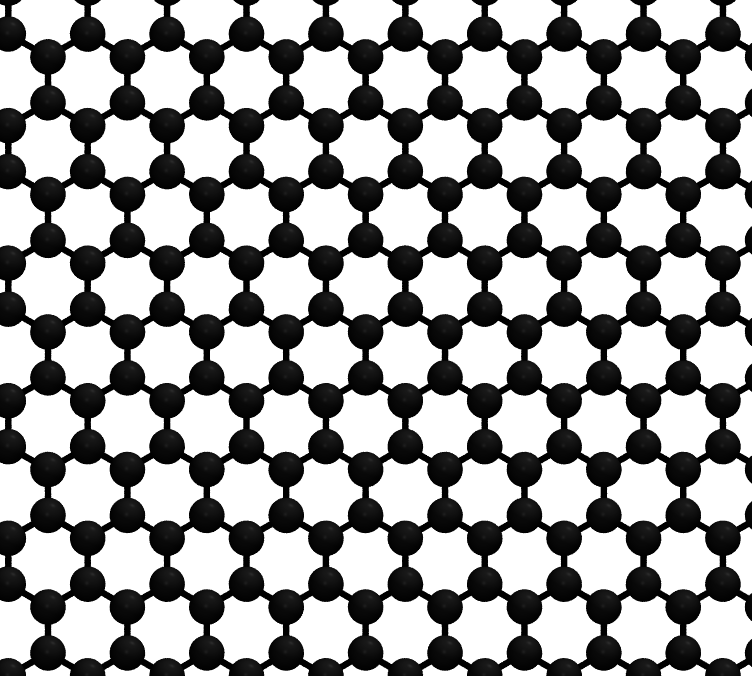
\includegraphics[width=7cm]{golddual/sheets/graphene.png}}\hspace{1cm}
	\subfloat[]{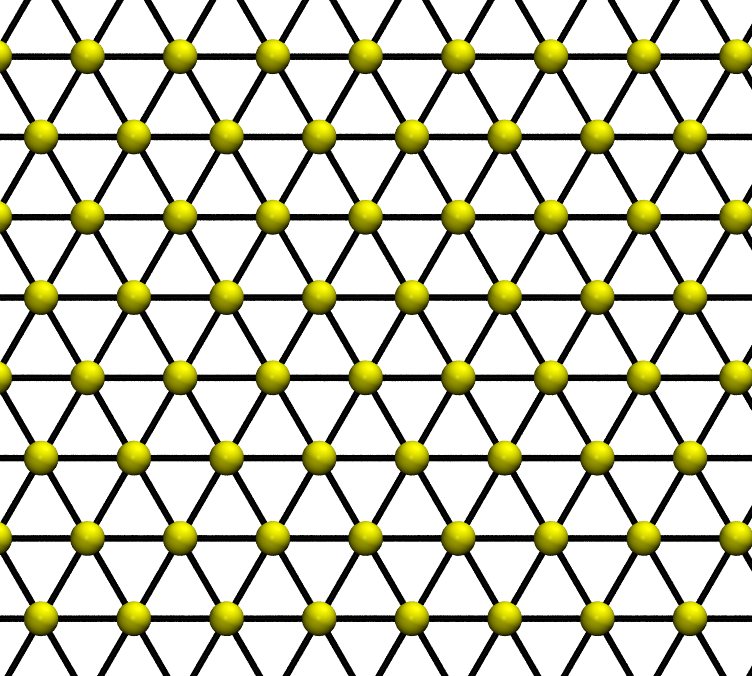
\includegraphics[width=7cm]{golddual/sheets/gold.png}}
\caption{(a) \textit{p3m1}-G graphene and (b) its dual sheet \textit{p3m1}-T adopted in (111) surface of fcc gold.}
\label{fig:graphenedual}
\end{center}
\end{figure*}

\begin{figure*}[htbp]
\begin{center}
	\subfloat[]{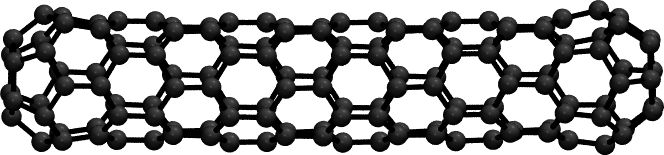
\includegraphics[width=10cm]{golddual/C144.png}} \\
	\subfloat[]{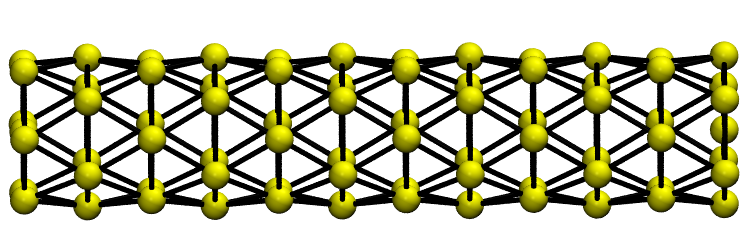
\includegraphics[width=10cm]{golddual/Au74.png}}
	\caption{(a) $D_{6d}-$C$_{144}$ zig-zag fullerene nanotube and (b) its dual $D_{6d}-$Au$_{74}$.}
\label{fig:nanotubedual}
\end{center}
\end{figure*}

The requirement to have 12 pentagons in a fullerene graph with $F_h$ hexagons ($F_h$=0 for C$_{20}$ and $F_h > 1$ for all other fullerenes) implies for a fullerene dual to have exactly 12 vertices of degree five and the remaining of degree six. In fact it is well known that C$_{22}$ cannot exist as a fullerene,\autocite{Grunbaum_numberhexagonssimplicity_1963} which implies that its hypothetical dual Au$_{13}$ does not exist either (the number of vertices $N_d$ in the dual is identical to the number of faces in a fullerene, $N_d=F_f=N_f/2+2$,\autocite{Schwerdtfeger_topologyfullerenes_2015} using symbols $f$ and $d$ for the fullerene and its dual respectively). Because there is a one-to-one correspondence between a fullerene and its dual graph, we have as many isomers (nonisomorphic graphs) for C$_{N_f}$ as we have for Au$_{N_f/2+2}$ and dualization preserves the point group symmetry. Here we mention that according to Thurston, the number of isomers increases polynomially in ninth leading order with the number of vertices, i.e. $\sim\mathcal{O}({N_f^9})$.\autocite{Thurston_Shapespolyhedratriangulations_1998} 

Au$_{32}$ was the first of such golden fullerenes postulated by Johansson et al. to be a rather stable hollow cluster, and they were the first ones mentioning that these golden dual fullerenes (GDF) are obtained from fullerene graphs.\autocite{Johansson_Au3224CaratGolden_2004} Au$_{32}$ is shown in Figure \ref{fig:C60dual} together with its dual, C$_{60}$ and the corresponding graph representation (twice the dual transformation leads back to the original polyhedron or graph). Now that we established an isomorphism between a fullerene graph and its dual, we can easily construct isomers of golden fullerenes by using standard algorithms for the construction of fullerenes, such as the generalized face-spiral algorithm,\autocite{Fowler-atlas-2006,Schwerdtfeger_Programfullerenesoftware_2013,Wirz-2014,Schwerdtfeger_topologyfullerenes_2015} embedding the graph on a genus 0 surface and finally transforming the cage to its dual.

\begin{figure*}[htbp]
\begin{center}
	\subfloat[]{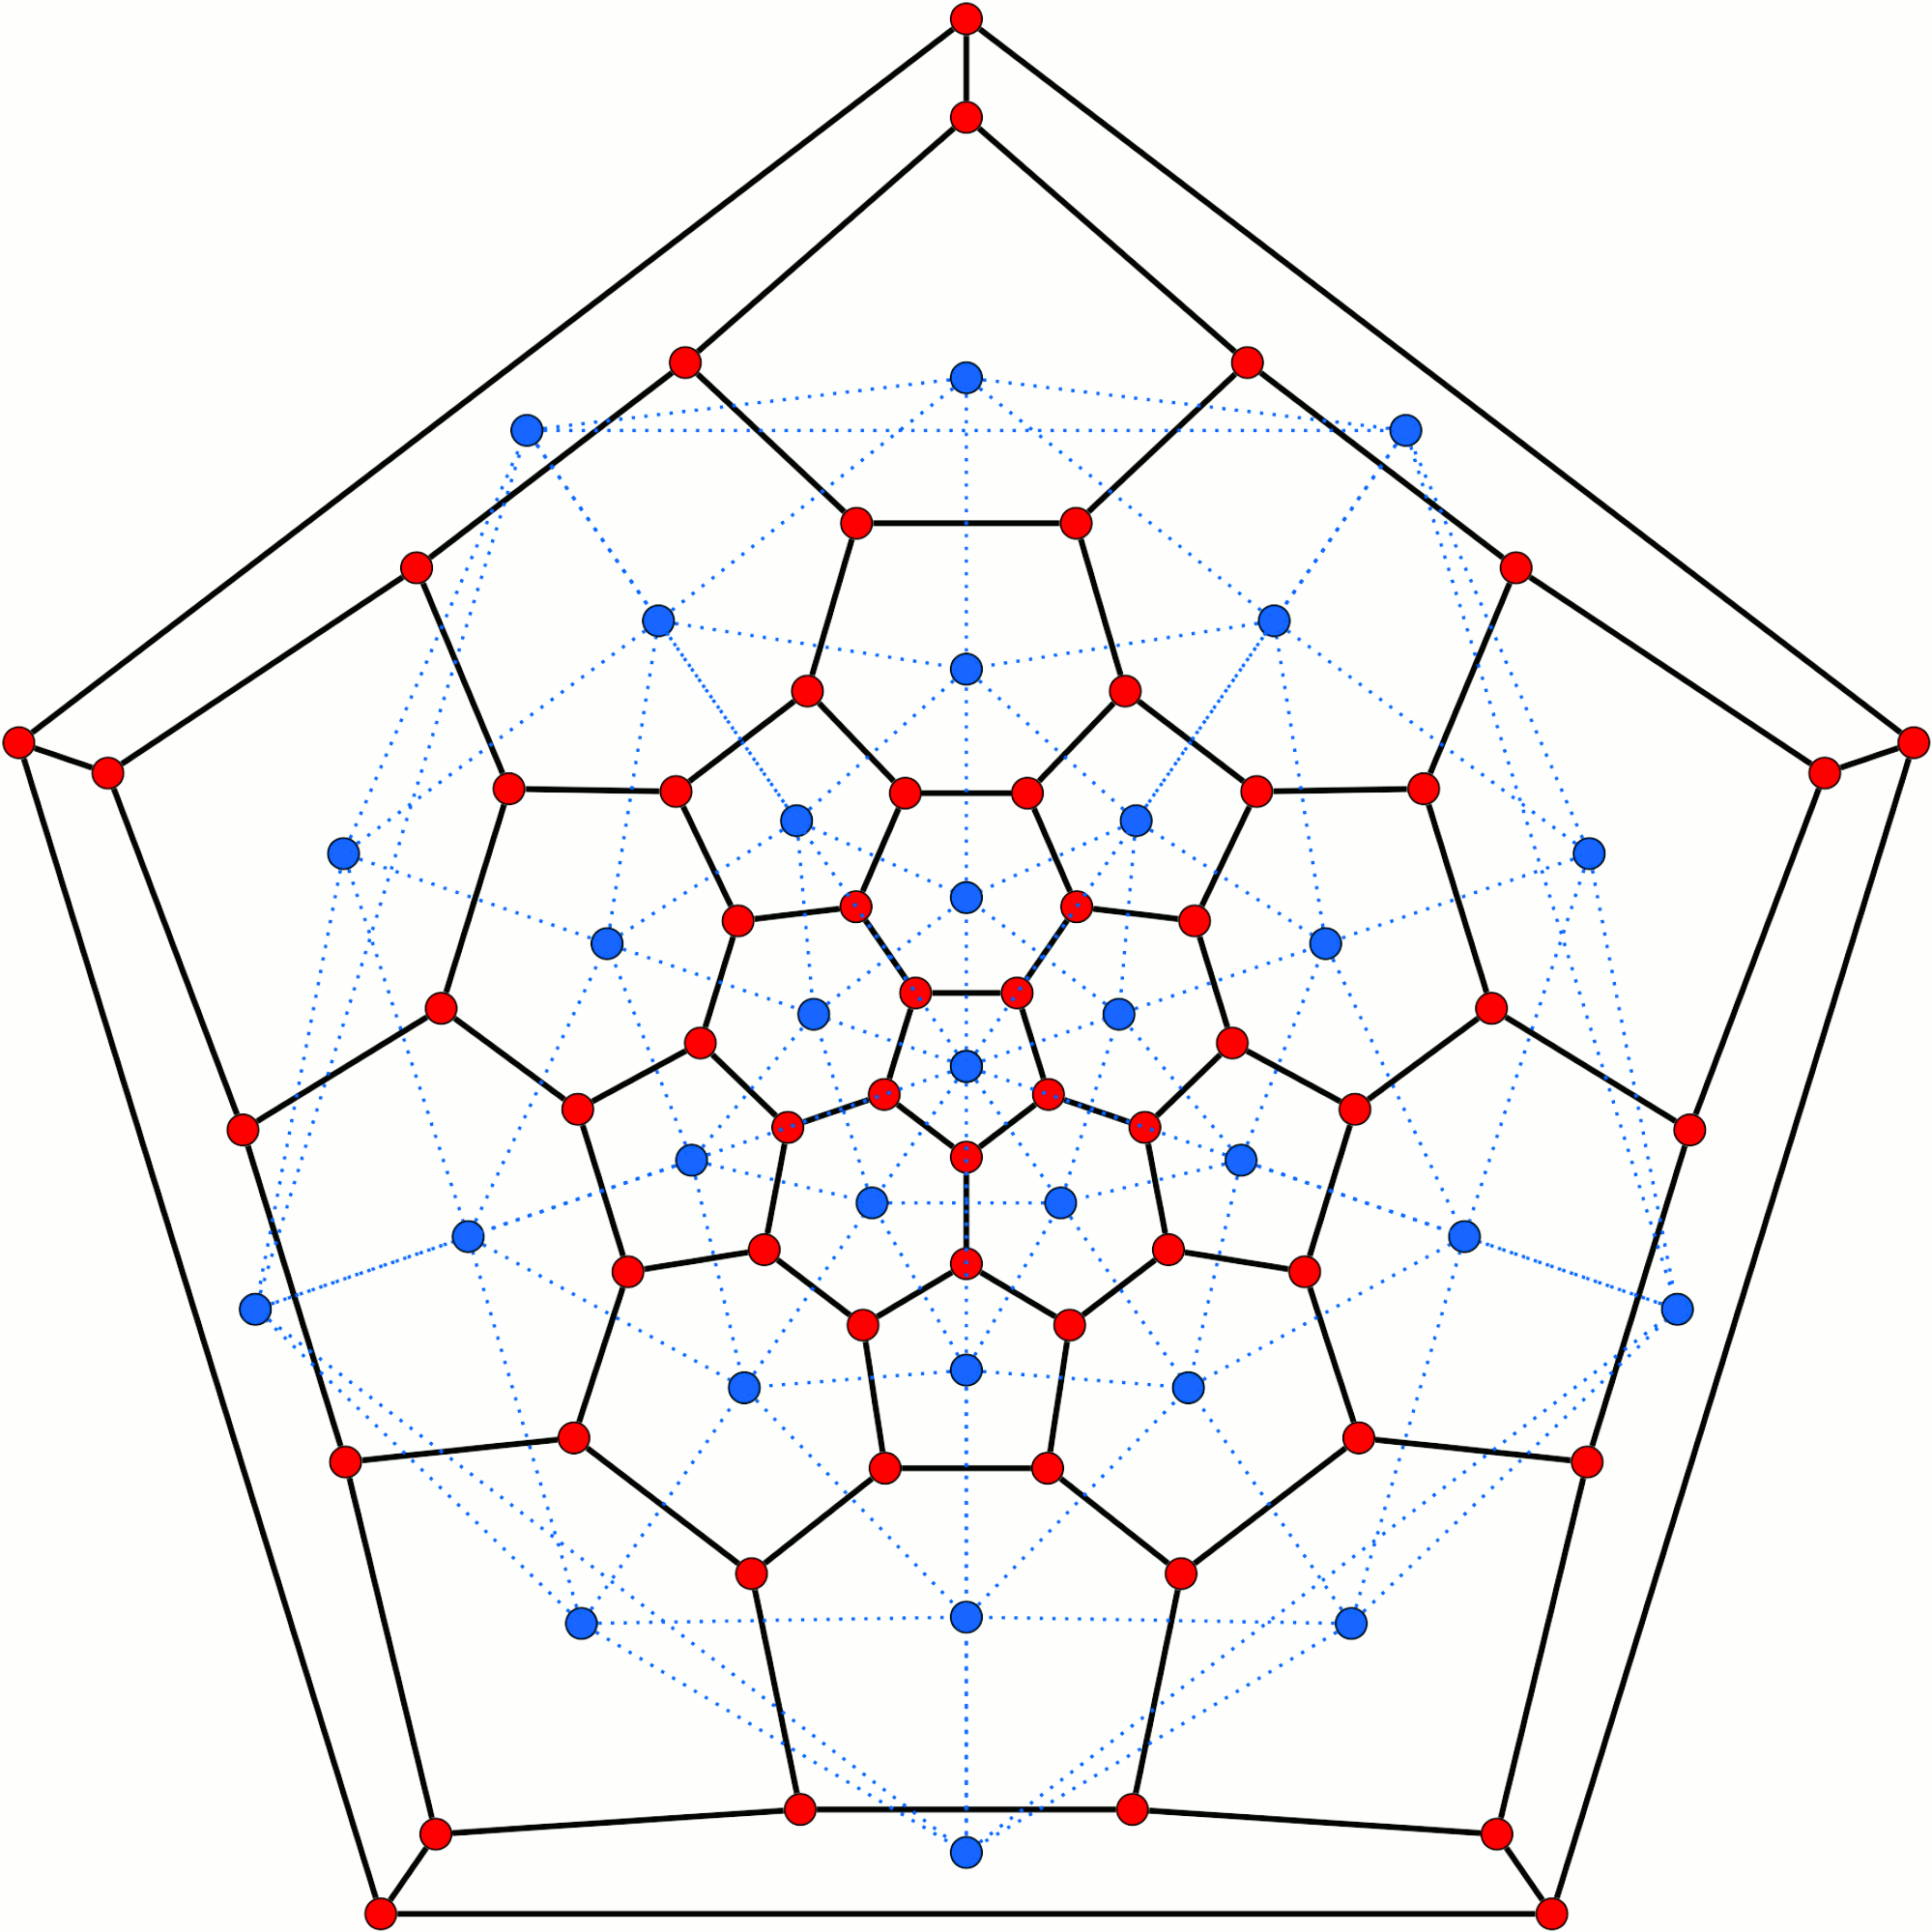
\includegraphics[width=.3\textwidth]{golddual/C60graph.png}}\hfill
    \subfloat[]{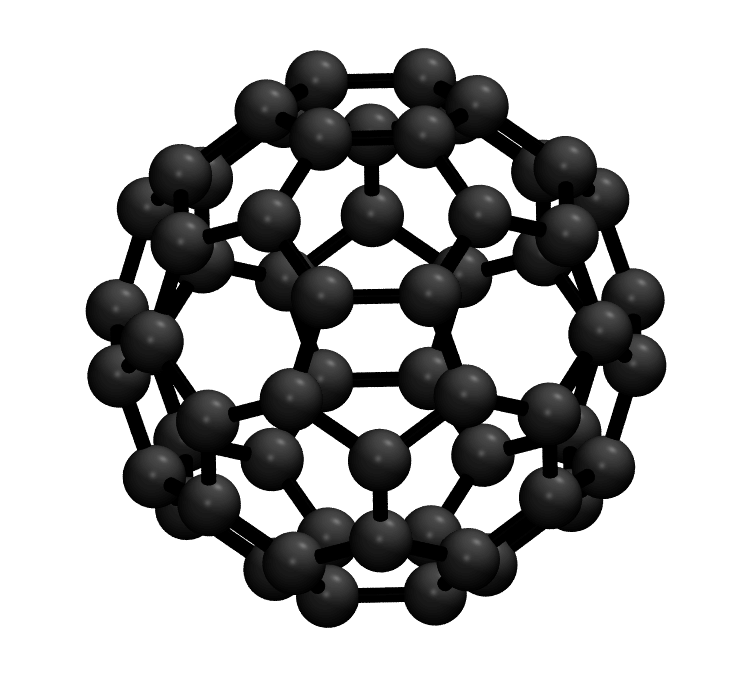
\includegraphics[width=.3\textwidth]{golddual/C60Ih.png}}\hfill
	\subfloat[]{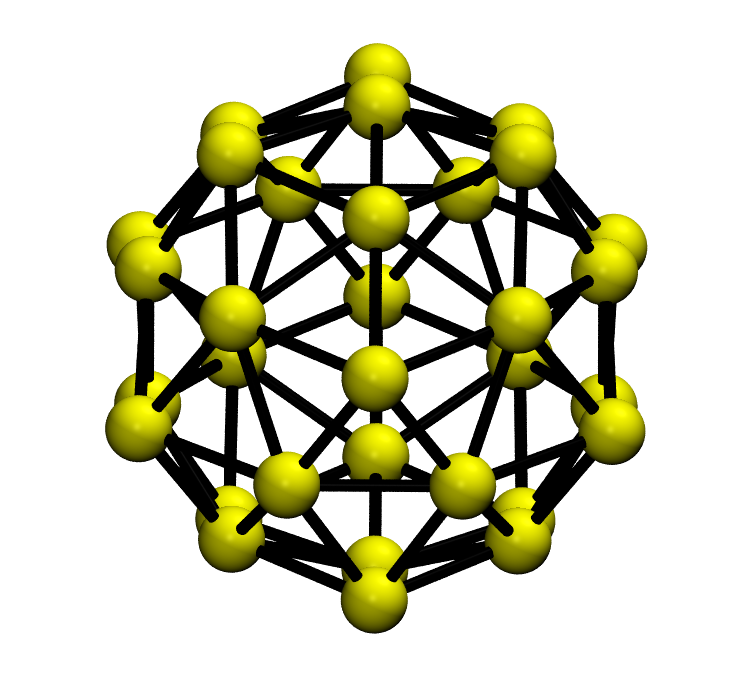
\includegraphics[width=.3\textwidth]{golddual/Au32Ih.png}}
\caption{(a) Schlegel diagram of C$_{60}$ (red vertices) and its dual (blue vertices and dashed edges), (b) the C$_{60}$ structure and (c) its dual Au$_{32}$ structure.}
\label{fig:C60dual}
\end{center}
\end{figure*}

As an example we mention Au$_{16}$ as the dual of C$_{28}$. Checking the list of possible isomers\autocite{Brinkmann_HouseGraphsdatabase_2013} we see that there are two possible non-isomorphic structures, $D_2-$Au$_{16}$ and $T_d-$Au$_{16}$. However, only the more symmetric $T_d-$Au$_{16}^-$ has been considered as a possible candidate in recent photoelectron spectroscopy experiments.\autocite{Bulusu_Evidencehollowgolden_2006} The question naturally arises if the other negatively charged $D_2$ isomer has a similar photoelectron spectrum and is more stable or not compared to the $T_d$ isomer. In fact, Au$_{32}$ which is the dual of C$_{60}$ has 1812 different isomers with only one fulfilling the isolated pentagon rule (IPR) as proposed by Kroto.\autocite{Kroto_stabilityfullerenesCn_1987} For example, in a recent paper Fa and Dong reported on a hollow gold $D_{6d}-$Au$_{26}$ cluster.\autocite{Fa-Dong-2006,Fa-Luong-2008} Looking at the list of possible fullerenes we see that there are 199 possible isomers for dual fullerene structures, and in fact there are two possible isomers having $D_{6d}$ symmetry. This just highlights the rich topology of such dual fullerenes.

For the dual structures we do not know if a similar rule applies, that is an ``isolated vertex rule'' of degree five (IVR5). In fullerenes the pentagons are responsible for the curvature of the carbon cage and for the overall symmetry and structure, with connected hexagons building planar sub-structures on the polyhedron. Here we mention that the Mackay icosahedron (discussed below) shows exactly that feature.

\textit{p3m1}-G sheets have been considered by Goldberg and Coxeter for the construction of larger fullerenes.\autocite{Goldberg_ClassMultiSymmetricPolyhedra_1937,Coxeter-1971,Dutour_GoldbergCoxeterConstructionvalent_2004} The original Goldberg-Coxeter transformation superimposes a hexagonal mesh on the surface of the C$_{20}$ dodecahedron forming a new polyhedron with leaving the number of pentagons at exactly 12.\autocite{Goldberg_ClassMultiSymmetricPolyhedra_1937,Coxeter-1971} This transformation can be applied to any fullerene isomer.\autocite{Schwerdtfeger_topologyfullerenes_2015} The Goldberg-Coxeter transformation $GC_{k,l}$ increases the number of vertices for a fullerene by a factor of $(k^2+kl+l^2)$, where $k$ and $l$ are integers describing the scale and orientation of the mesh.\autocite{Dutour_GoldbergCoxeterConstructionvalent_2004,Schwerdtfeger_topologyfullerenes_2015} If $k=l$ or $l=0$ the point group symmetry is preserved. For example, we have $GC_{1,1}$[$I_h-$C$_{20}$]=$I_h-$C$_{60}$ (leapfrog transformation)\autocite{Fowler-atlas-2006} and $GC_{2,0}$[$I_h-$C$_{20}$]=$I_h-$C$_{80}$ (halma transformation), or in the dual case applying the same procedure to the \textit{p3m1}-T sheet for our gold fullerenes $GC_{1,1}$[$I_h-$Au$_{12}$]=$I_h-$Au$_{32}$ and $GC_{2,0}$[$I_h-$Au$_{12}$]= $I_h-$Au$_{42}$. Simple algebra shows that $GC_{k,l}$[Au$_{N_d}$] has a new vertex count of
\begin{equation}
  \label{eq:dualvertex} 
N_d'=(k^2+kl+l^2)(N_d-2)+2 
\end{equation}
Both $I_h-$Au$_{32}$ and $I_h-$Au$_{42}$ have been postulated as stable golden fullerenes before,\autocite{Johansson_Au3224CaratGolden_2004}
and more recently the chiral $I-$Au$_{72}$\autocite{Karttunen_IcosahedralAu72_2008} which is nothing else as the dual of $GC_{2,1}$[$I_h-$C$_{20}$] = $I-$C$_{140}$, which is chiral as well as symmetry is conserved upon dualization.

Now it almost seems trivial to relate Mackay icosahedra\autocite{Mackay-1962} well known for gold clusters\autocite{Nam2002,Wang-Wang-2011} to fullerenes. We might call them "multi-walled halma-transformed icosahedral" dual fullerenes in analogous way to the multi-walled gold nanowires. A Mackay icosahedron is a closed packed multi-shell structure each shell being an icosahedron with
\begin{equation}
  \label{eq:mackay} 
N_{shell}=10k^2+2
\end{equation}
number of atoms in each shell with increasing $k$. This gives the well known magic cluster numbers of (including the central atom) 13, 55, 147, 309, 561, ... derived from
\begin{equation}
  \label{eq:mackaytotal} 
N_{total}=1+2\sum_{k=1}^{m_{shell}}\left( 5k^2+1 \right)=(10m_{shell}^3+15m_{shell}^2+11m_{shell}+3)/3
\end{equation}
with $m_{shell} \ge 1$. One such Mackay icosahedron with $m_{shell}$=7 and $N_{total}$=1415 is shown in Figure \ref{fig:mackaylarge}. The triangles clearly show the halma pattern of a Goldberg-Coxeter $GC_{k,0}$ transformation. Because each transformation brings a new vertex on the icosahedral edge, we can just deduct the number of shells by counting the number of atoms at one edge of a triangle $N_{edge}$, i.e. $m_{shell}=N_{edge}-1$, which gives 8 atoms and 7 icosahedral shells for the Mackay icosahedron shown in Figure \ref{fig:mackaylarge}.
\begin{figure*}[htbp]
\begin{center}
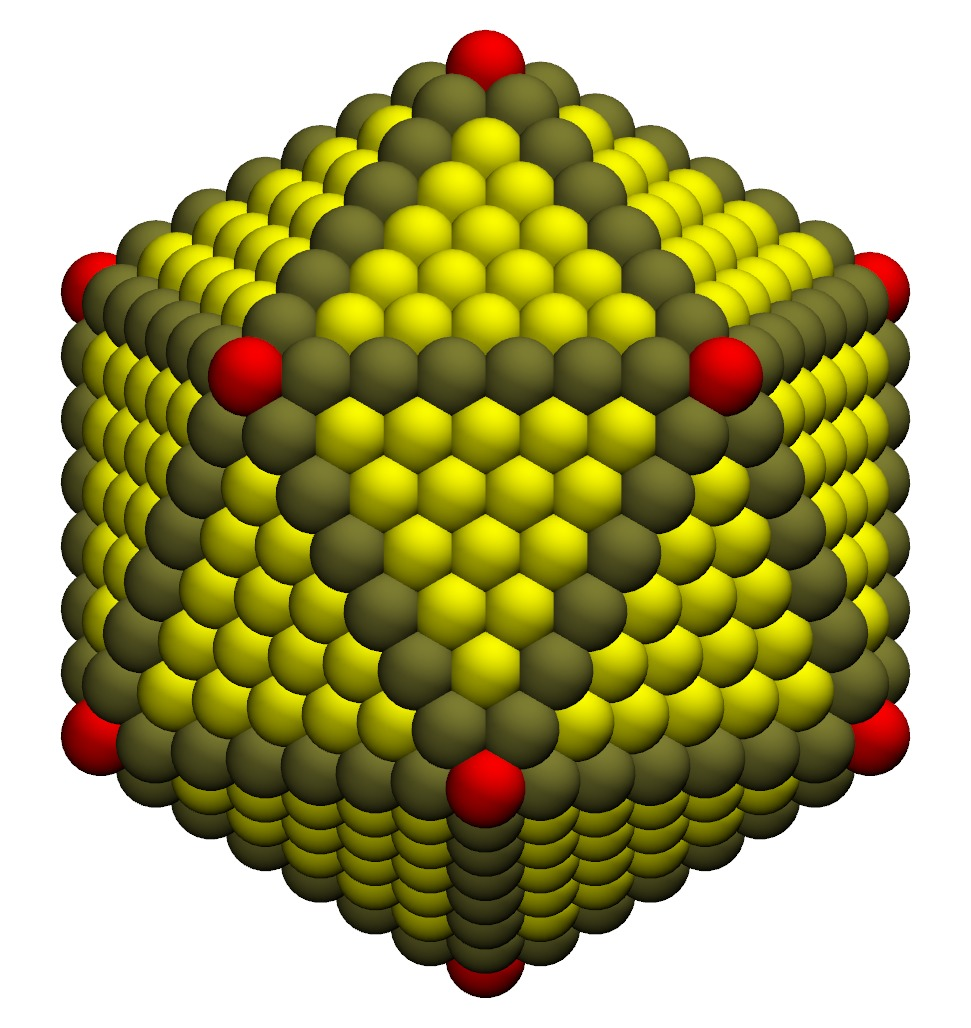
\includegraphics[width=4.9cm]{golddual/ico.jpg}
\caption{Mackay icosahedron with 7 shells and 1415 atoms. The outer icosahedral shell is the dual of the halma transform $GC_{7,0}$[$I_h-$C$_{20}$]=$I_h-$C$_{980}$.}
\label{fig:mackaylarge}
\end{center}
\end{figure*}
Mackay pointed out that the packing density (or atomic packing factor) for $N \rightarrow \infty$ with $\rho$=0.68818 is not too different from a closed packed structure such as fcc with $\rho=\pi/\sqrt{18}$=0.74048,\autocite{Mackay-1962} one reason why icosahedral cluster growth is often seen. The number of atoms in a shell $N_{shell}$ directly corresponds to the number of faces in a halma transformed C$_{20}$, i.e. for $l=0$ in the Goldberg-Coxeter transformation and starting with $N_d$=12 in eq.\ref{eq:dualvertex} we have $N_d'=k^2(N_d-2)+2 = 10k^2+2$ identical with the formula given by Mackay. 

Finally we mention that we can name the different isomers of the golden dual fullerenes exactly in the same way as we do for the fullerenes by using the canonical face spiral pentagon indices (FSPI) and the numbering scheme introduced by Fowler and Manolopoulos,\autocite{Fowler-atlas-2006} keeping in mind that the face spiral for fullerenes now becomes a vertex spiral for the dual triangulated surface. We are now turning to a detailed analysis of all possible golden dual fullerenes from $I_h-$Au$_{12}$, Au$_{14}$ to Au$_{20}$ and $I_h-$Au$_{32}$ by quantum chemical calculations.

%Computational Details
\section{\label{sec:CompDet}Computational Details}

Program FULLERENE\autocite{Schwerdtfeger_Programfullerenesoftware_2013} has been used to construct initial
structures of all isomers of the golden dual fullerenes from Au$_{12}$ to
Au$_{20}$ using a recently developed force-field for
fullerenes\autocite{Wirz_smallfullerenesgraphene_2015} (as already mentioned the golden dual fullerene
Au$_{13}$ does not exist). The following isomers need to be considered
according to the isomer list for the fullerenes (number in parenthesis gives
the number of different isomers of same symmetry):\autocite{Brinkmann_HouseGraphsdatabase_2013,Schwerdtfeger_Programfullerenesoftware_2013}
$I_h-$Au$_{12}$, $D_{6d}-$Au$_{14}$, $D_{3h}-$Au$_{15}$, $D_{2}-$Au$_{16}$,
$T_{d}-$Au$_{16}$, $D_{5h}-$Au$_{17}$, $C_{2v}-$Au$_{17}$(2),
$D_{3h}-$Au$_{18}$, $D_{3d}-$Au$_{18}$, $D_{3}-$Au$_{18}$, $D_{2}-$Au$_{18}$,
$C_{3}-$Au$_{18}$(2), $C_{3v}-$Au$_{19}$, $C_{2}-$Au$_{19}$(3),
$C_{s}-$Au$_{19}$(2), $D_{6h}-$Au$_{20}$, $D_{3h}-$Au$_{20}$,
$D_{2d}-$Au$_{20}$(2), $C_{2v}-$Au$_{20}$, $D_{2}-$Au$_{20}$(2),
$C_{2}-$Au$_{20}$(3), $C_{2}-$Au$_{20}$(2), $C_{1}-$Au$_{20}$(2) and
$I_h-$Au$_{32}$. The initial force-field optimized structures scaled to an
approximate internuclear distance were then refined by using the
Perdew-Becke-Ernzerhofer generalized gradient
functional\autocite{Perdew_GeneralizedGradientApproximation_1996,PerdewGeneralizedGradientApproximation1997} corrected for dispersion interactions
using Grimme's method (PBE-D3)\autocite{Grimme_consistentaccurateinitio_2010,Grimme_Effectdampingfunction_2011} together with a Los-Alamos
scalar relativistic effective core potential for gold and the accompanying
double-zeta basis sets.\autocite{Wadt1985} Note that the PBE functional was recently
considered to perform well for gold clusters.\autocite{Mancera_alternativemethodologyassess_2015} For several
selected clusters we checked that the geometries obtained were accurate by
performing calculations using a small core scalar relativistic Stuttgart
pseudopotential\autocite{Figgen_Energyconsistentpseudopotentialsgroup_2005} together with an augmented valence double-zeta
basis set of Peterson and Puzzarini.\autocite{Peterson-2005} In comparison, we also
calculated the compact global minimum cluster structures which were recently
published for the neutral compounds by our group\autocite{Assadollahzadeh_systematicsearchminimum_2009} and
for the negatively charged species by Kappes and
co-workers.\autocite{Schooss_Determiningsizedependentstructure_2010,Lechtken_Structuredeterminationgold_2009}

The simulation of the photoelectron spectra has been carried out by artificial
broadening the spectrum of orbital energies with Gaussian functions. The standard deviation $\sigma$
for these functions was chosen to be 0.035~eV in qualitative agreement with the experimental spectra. The orbital energies were
calculated using the PBE density functional with the def2-SVP\autocite{Weigend_Balancedbasissets_2005} double zeta basis
implemented in TURBOMOLE 7.0.\autocite{_TURBOMOLEV72015_} The core region was described using an effective
core potential including scalar relativistic effects.
The calculated electron affinities were used as the onset value for simulating the photoelectron spectra. 


For the calculation of the (111) fcc sheet and the fcc bulk structure of gold we used the program package VASP5\autocite{Kresse_Efficiencyabinitiototal_1996} utilizing a plane-wave basis set (cutoff energy $E_c=350$~eV) and the standard projector-augmented wave (PAW) datasets for the elements to model the electron-ion interaction\autocite{Blochl_Projectoraugmentedwavemethod_1994,Kresse_ultrasoftpseudopotentialsprojector_1999}. The electron-electron interaction was modelled within the generalised gradient approximation to the exchange-correlation energy functional as described above and dispersive effects were taken into account by employing Grimme's D3 dispersion correction with Becke-Johnson damping.\autocite{Grimme_consistentaccurateinitio_2010,Grimme_Effectdampingfunction_2011} Brillouin zone integrations were performed on $\Gamma$-centered Monkhorst-Pack grids of $k$-points with a distance of 0.2~\AA$^{-1}$.
The cohesive energy is defined as the atomization energy per atom keeping in mind that one gold atom is negatively charged for the anionic clusters.

In order to discuss how much the gold cages deviate from sphericity compared to the dual fullerene structure we use the previously introduced definition of a minimum distance sphere (MDS),\autocite{Schwerdtfeger_Programfullerenesoftware_2013}
\begin{equation} 
\min\limits_{c_\mathrm{MDS} \in \mathrm{CH}(S)} \frac{1}{N} \sum _{i} \left|R_\mathrm{MDS} -\| \vec{p}_{i}-\vec{c}_\mathrm{MDS} \| \right|  
\end{equation}
with the MDS radius defined as
\begin{equation} 
	R_{\mathrm{MDS}} =\frac{1}{N} \sum _{i}\| \vec{p}_{i} -\vec{c}_{\mathrm{MDS}} \|   
	\label{eq:RMDS}
\end{equation}
Here $S$ is the set of $n$ points $\vec{p}_i$ ($i=1,\ldots ,N$) in $3$-dimensional space, CH($S$) its convex hull, $\|\cdot\| $ the Euclidean norm, and $\vec{c}_\mathrm{MDS}$ is the barycenter of the MDS with radius $R_\mathrm{MDS}$. In other words, we look for a sphere with the vertices lying inside or outside the sphere, but closest to it. We now define a measure for distortion from spherical symmetry through the MDS,\autocite{Schwerdtfeger_Programfullerenesoftware_2013}
\begin{equation}
  \label{eq:DMDS}
  D_{\mathrm{MDS}} = \frac{100}{N R_\mathrm{min}} \sum_{i=1}^N \left|R_{\mathrm{MDS}} - \|\vec{p}_i - \vec{c}_{\mathrm{MDS}}\| \right|
\end{equation}
where $R_\mathrm{min}$ is the smallest bond distance found in the cluster. The pentagon index $N_p$ is defined as
\begin{equation}
  \label{pentindex}
  N_p = \frac{1}{2}\sum_{k=1}^{5} kp_k \quad \text{ with } \quad  \sum_{k=0}^{5} p_k = 12
\end{equation}
where the pentagon indices $(p_i | i=0, \dots , 5)$ define the number of pentagons attached to another pentagon.\autocite{Fowler-atlas-2006}


\section{\label{sec:ResDis}Results and Discussion}
\subsection{Structure and Stability}

The results for the neutral and negatively charged gold clusters are collected in
Tables \ref{tab:neutral} and \ref{tab:anion} respectively. The dual fullerene
structures (DF) are compared to the known global minimum (GM) structures in
these tables, and the different isomers are numbered according to their
canonical degree 5 vertex spiral identical to the canonical face spiral
pentagon indices for fullerenes.\autocite{Fowler-atlas-2006} We also include
calculations for the most stable neutral and anionic compact Au$_n$
clusters for comparison which are listed in Table \ref{tab:Aun}. The
investigated structures for the
negatively charged gold clusters are depicted in Figures \ref{fig:Au1219-} and
\ref{fig:Au20-}, and the energy differences compared to the global minimum structures
are shown in Figure~\ref{fig:AunMinus2}.

\begin{table}[ht!]
	\centering
    \setlength{\tabcolsep}{3pt}
    \small{
    \caption{Topological parameters for the neutral gold clusters. Number of
    gold atoms and isomer numbers of the corresponding fullerene in canonical
    order of the pentagon spiral indices,\autocite{Fowler-atlas-2006} ideal and
    actual point group symmetry, energy differences $\Delta E_g$ to the most
    stable neutral cluster of same size and binding energy per atom $\Delta E_n
    = [E(\textrm{Au}_n)-nE(\textrm{Au})]/n$  (in eV), shortest and largest bond
    distance (in \AA), pentagon index (PI) $N_p$, and distortion parameter $D$
    (in \%) for the initial force-field optimized fullerene structure (F) and
    the dual gold cluster (GDF).}
	\label{tab:neutral}
	\begin{tabular}{lllrrrrrrrrrrrr}
\toprule
\multicolumn{1}{c}{  } & \multicolumn{2}{c}{ symmetry  }  & \multicolumn{2}{c}{stability} & \multicolumn{4}{c}{ vertices } & & \multicolumn{2}{c}{ bondlengths } &  PI & \multicolumn{2}{c}{ distortion } \\
isomer & ideal  & actual  & $\Delta E_n$ &$\Delta E_g$ & \multicolumn{1}{c}{$N_4$} & \multicolumn{1}{c}{$N_5$} & \multicolumn{1}{c}{$N_6$} & \multicolumn{1}{c}{$N_7$} & $\Gamma$ & shortest & largest  & $N_p$ & $D(\textrm{F})$ & $D(\textrm{GDF})$\\\midrule
12:1    & $I_h$    & $D_{4h}$ & $-2.058$ & $0.485$  & $8$ & $0$  & $4$      & $0$ & 16 & $2.798$ & $2.895$ & 30  & 0    &  21.1    \\
14:1    & $D_{6d}$ & $D_{2d}$ & $-2.134$ & $1.173$  & $0$ & $12$ & $2$      & $0$ & 12 & $2.739$ & $3.048$ & 24  & 6.1  &  23.4    \\
15:1    & $D_{3h}$ & $C_{2v}$ & $-2.192$ & $-0.083$ & $0$ & $12$ & $3$      & $0$ & 12 & $2.786$ & $2.901$ & 21  & 5.1  &  29.2    \\
16:1    & $D_2$    & $D_{2 }$ & $-2.247$ & $0.223$  & $0$ & $12$ & $4$      & $0$ & 12 & $2.770$ & $2.917$ & 20  & 7.9  &  24.3    \\
16:2    & $T_d$    & $D_{2d}$ & $-2.233$ & $0.440$  & $0$ & $12$ & $4$      & $0$ & 12 & $2.716$ & $2.996$ & 18  & 1.3  &  28.5    \\
17:1    & $D_{5h}$ & $C_s$*   & $-2.259$ & $0.177$  & $2$ & $8$  & $3$      & $3$ & 12 & $2.747$ & $3.026$ & 20  & 11.5 &  17.3    \\
17:2    & $C_{2v}$ & $C_{2v}$ & $-2.272$ & $-0.038$ & $0$ & $12$ & $5$      & $0$ & 12 & $2.769$ & $2.931$ & 18  & 7.6  &  19.1    \\
17:3    & $C_{2v}$ & $C_{2v}$ & $-2.277$ & $-0.128$ & $0$ & $12$ & $5$      & $0$ & 12 & $2.762$ & $3.139$ & 17  & 5.5  &  20.8    \\
18:1    & $C_2$    & $C_{2 }$ & $-2.307$ & $0.321$  & $0$ & $12$ & $6$      & $0$ & 12 & $2.736$ & $2.934$ & 17  & 9.2  &  16.9    \\
18:2    & $D_2$    & $D_{2 }$ & $-2.290$ & $0.627$  & $0$ & $12$ & $6$      & $0$ & 12 & $2.733$ & $2.935$ & 18  & 11.6 &  17.2    \\
18:3    & $D_{3d}$ & $D_{3d}$ & $-2.275$ & $0.896$  & $0$ & $12$ & $6$      & $0$ & 12 & $2.714$ & $2.894$ & 18  & 12.1 &  18.2    \\
18:4    & $C_2$    & $C_{2 }$ & $-2.321$ & $0.073$  & $0$ & $12$ & $6$      & $0$ & 12 & $2.749$ & $2.931$ & 16  & 7.2  &  18.7    \\
18:5    & $D_{3h}$ & $D_{3h}$ & $-2.303$ & $0.386$  & $0$ & $12$ & $6$      & $0$ & 12 & $2.763$ & $3.159$ & 8   & 15.1 &  27.3    \\
18:6    & $D_3$    & $D_{3 }$ & $-2.310$ & $0.270$  & $0$ & $12$ & $6$      & $0$ & 12 & $2.742$ & $2.945$ & 15  & 5.8  &  15.2    \\
19:1    & $C_2$    & $C_{2 }$ & $-2.298$ & $1.196$  & $0$ & $12$ & $7$      & $0$ & 12 & $2.745$ & $3.006$ & 17  & 14.9 &  26.0    \\
19:2    & $C_s$    & $C_{s }$ & $-2.307$ & $1.014$  & $0$ & $12$ & $7$      & $0$ & 12 & $2.747$ & $2.972$ & 15  & 7.5  &  20.0    \\
19:3    & $C_s$    & $C_{s }$ & $-2.304$ & $1.077$  & $0$ & $12$ & $7$      & $0$ & 12 & $2.737$ & $2.957$ & 15  & 11.9 &  28.3    \\
19:4    & $C_2$    & $C_{2 }$ & $-2.311$ & $0.935$  & $0$ & $12$ & $7$      & $0$ & 12 & $2.745$ & $2.905$ & 15  & 7.0  &  17.7    \\
19:5    & $C_2$    & $C_{2 }$ & $-2.313$ & $0.911$  & $0$ & $12$ & $7$      & $0$ & 12 & $2.734$ & $2.947$ & 14  & 6.6  &  18.7    \\
19:6    & $C_{3v}$ & $C_{3v}$ & $-2.316$ & $0.854$  & $0$ & $12$ & $7$      & $0$ & 12 & $2.765$ & $2.890$ & 15  & 12.7 &  30.6    \\
20:1    & $C_2$    & $C_{1 }$ & $-2.324$ & $1.684$  & $2$ & $8$  & $10$     & $0$ & 12 & $2.711$ & $2.984$ & 16  & 15.3 &  36.7    \\
20:2    & $D_2$    & $D_{2 }$ & $-2.295$ & $2.271$  & $0$ & $12$ & $8$      & $0$ & 12 & $2.699$ & $3.023$ & 18  & 20.4 &  22.0    \\
20:3    & $C_1$    & $C_{1 }$ & $-2.339$ & $1.395$  & $2$ & $8$  & $10$     & $0$ & 12 & $2.724$ & $2.954$ & 15  & 13.1 &  129.1   \\
20:4    & $C_s$    & $C_{s }$ & $-2.324$ & $1.695$  & $0$ & $12$ & $8$      & $0$ & 12 & $2.709$ & $3.023$ & 16  & 13.7 &  25.5    \\
20:5    & $D_2$    & $D_{2 }$ & $-2.332$ & $1.541$  & $0$ & $12$ & $8$      & $0$ & 12 & $2.749$ & $3.080$ & 16  & 18.5 &  17.3    \\
20:6    & $D_{2d}$ & $C_{2v}$ & $-2.337$ & $1.440$  & $2$ & $8$  & $10$     & $0$ & 12 & $2.752$ & $2.977$ & 14  & 9.8  &  26.6    \\
20:7    & $C_1$    & $C_{1 }$ & $-2.325$ & $1.663$  & $2$ & $9$  & $8$      & $1$ & 12 & $2.712$ & $3.019$ & 14  & 10.9 &  25.8    \\
20:8    & $C_s$    & $C_{s }$ & $-2.346$ & $1.256$  & $2$ & $8$  & $10$     & $0$ & 12 & $2.748$ & $3.057$ & 14  & 8.4  &  40.7    \\
20:9    & $C_{2v}$ & $D_{6h}$ & $-2.362$ & $0.938$  & $6$ & $0$  & $14$     & $0$ & 12 & $2.744$ & $2.971$ & 13  & 3.8  &  23.2    \\
20:10   & $C_2$    & $C_{2 }$ & $-2.344$ & $1.299$  & $2$ & $8$  & $10$     & $0$ & 12 & $2.726$ & $3.004$ & 14  & 12.6 &  23.9    \\
20:11   & $C_2$    & $C_{s }$ & $-2.346$ & $1.256$  & $2$ & $8$  & $10$     & $0$ & 12 & $2.747$ & $3.056$ & 13  & 8.1  &  35.8    \\
20:12   & $C_2$    & $C_1$ c  & $-2.366$ & $0.861$  & $3$ & $5$  & $4$      & $7$ & 4  & $2.719$ & $3.048$ & 13  & 5.4  &  21.1    \\
20:13   & $D_{3h}$ & $D_{6h}$ & $-2.362$ & $0.938$  & $6$ & $0$  & $14$     & $0$ & 12 & $2.744$ & $2.970$ & 15  & 6.5  &  27.9    \\
20:14   & $D_{2d}$ & $D_{2d}$ & $-2.311$ & $1.948$  & $0$ & $12$ & $8$      & $0$ & 12 & $2.779$ & $2.929$ & 12  & 3.7  &  22.0    \\
20:15   & $D_{6h}$ & $D_{6h}$ & $-2.362$ & $0.936$  & $6$ & $0$  & $14$     & $0$ & 12 & $2.744$ & $2.972$ & 12  & 4.5  &  25.6    \\
32:1082 & $I_h$    & $I_h$    & $-2.494$ & $1.537$  & $0$ & $12$ & $20$     & $0$ & 12 & $2.793$ & $2.835$ & 0   & 0    &  7.5   \\
(111)   & 2D       & sheet    & $-2.994$ &          & $0$ & $0$  & $\infty$ & $0$ &    & $2.722$ & $2.722$ & 0   & 0    & 0   \\
fcc     & 3D       & bulk     & $-3.677$ &          & $-$ & $-$  & $-$      & $-$ &    & $2.897$ & $2.897$ & $-$ & $-$  & $-$ \\
		\bottomrule
    \end{tabular}}
\end{table}


\begin{table}[ht!]
	\centering
    \footnotesize{
    \caption{Topological parameters for the anionic gold clusters. Number of
    gold atoms and isomer numbers of the fullerene in canonical order of the
    pentagon spiral indices,\autocite{Fowler-atlas-2006} ideal and actual point
    group symmetry, energy differences $\Delta E_g$ to the most stable anionic
    cluster of same size and binding energy per atom $\Delta E_n =
    [E(\textrm{Au}_n)-(n-1)E(\textrm{Au})-E(\textrm{Au}^-)]/n$  (in eV),
    shortest and largest bond distance (in \AA), and distortion parameter $D$
    (in \%) for the dual gold cluster (GDF). }
	\label{tab:anion}
\begin{tabular}{lllrrrrrrrrrr}
\toprule
\multicolumn{1}{c}{  } & \multicolumn{2}{c}{ symmetry  }  & \multicolumn{2}{c}{stability} & \multicolumn{4}{c}{ vertices } & & \multicolumn{2}{c}{ bondlengths } &  distortion \\
isomer & ideal  & actual  & $\Delta E_n$ &$\Delta E_g$ & \multicolumn{1}{c}{$N_4$} & \multicolumn{1}{c}{$N_5$} & \multicolumn{1}{c}{$N_6$} & \multicolumn{1}{c}{$N_7$}& $\Gamma$ & shortest & largest   & $D(\textrm{GDF})$  \\\midrule
12:1    & $I_h$    & $D_{2d}$  & $-2.137$ & $0.665$  & $8$ & $0$  & $4$  & $0$ & 16 & $2.780$ & $2.869$  &  23.0 \\
14:1    & $D_{6d}$ & $D_{2d}$  & $-2.242$ & $-0.089$ & $0$ & $12$ & $2$  & $0$ & 12 & $2.758$ & $2.989$  &  20.3 \\
15:1    & $D_{3h}$ & $C_{2v}$  & $-2.281$ & $0.473$  & $0$ & $12$ & $3$  & $0$ & 12 & $2.741$ & $3.029$  &  21.2 \\
16:1    & $D_2$    & $D_{2 }$  & $-2.328$ & $0.020$  & $0$ & $12$ & $4$  & $0$ & 12 & $2.764$ & $2.905$  &  17.7 \\
16:2    & $T_d$    & $D_{2d}$  & $-2.330$ & $0.000$  & $0$ & $12$ & $4$  & $0$ & 12 & $2.738$ & $2.907$  &  16.2 \\
17:1    & $D_{5h}$ & $D_{5h}$  & $-2.353$ & $0.469$  & $0$ & $12$ & $5$  & $0$ & 12 & $2.757$ & $3.017$  &  13.2 \\
17:2    & $C_{2v}$ & $C_{2v}$  & $-2.368$ & $0.215$  & $0$ & $12$ & $5$  & $0$ & 12 & $2.742$ & $2.994$  &  14.4 \\
17:3    & $C_{2v}$ & $C_{2v}$  & $-2.376$ & $0.087$  & $0$ & $12$ & $5$  & $0$ & 12 & $2.731$ & $3.019$  &  14.2 \\
18:1    & $C_2$    & $C_{2 }$  & $-2.360$ & $0.589$  & $0$ & $12$ & $6$  & $0$ & 12 & $2.734$ & $2.968$  &  16.8 \\
18:2    & $D_2$    & $C_{2 }$  & $-2.346$ & $0.848$  & $0$ & $12$ & $6$  & $0$ & 12 & $2.733$ & $3.059$  &  16.8 \\
18:3    & $D_{3d}$ & $C_{2 }$  & $-2.348$ & $0.817$  & $4$ & $4$  & $10$ & $0$ & 12 & $2.701$ & $3.038$  &  24.3 \\
18:4    & $C_2$    & $C_{1 }$  & $-2.364$ & $0.529$  & $0$ & $12$ & $6$  & $0$ & 12 & $2.740$ & $3.048$  &  19.0 \\
18:5    & $D_{3h}$ & $D_{3h}$  & $-2.364$ & $0.516$  & $0$ & $12$ & $6$  & $0$ & 12 & $2.710$ & $3.023$  &  27.5 \\
18:6    & $D_3$    & $D_{3 }$  & $-2.357$ & $0.642$  & $0$ & $12$ & $6$  & $0$ & 12 & $2.734$ & $2.912$  &  14.7 \\
19:1    & $C_2$    & $C_{2 }$  & $-2.384$ & $0.967$  & $4$ & $4$  & $11$ & $0$ & 12 & $2.732$ & $2.985$  &  28.5 \\
19:2    & $C_s$    & $C_{s }$  & $-2.368$ & $1.268$  & $2$ & $9$  & $7$  & $1$ & 12 & $2.727$ & $2.989$  &  16.9 \\
19:3    & $C_s$    & $C_{3v}$  & $-2.381$ & $1.022$  & $0$ & $12$ & $7$  & $0$ & 12 & $2.755$ & $3.046$  &  32.6 \\
19:4    & $C_2$    & $C_{2 }$  & $-2.390$ & $0.853$  & $2$ & $8$  & $9$  & $0$ & 12 & $2.744$ & $3.003$  &  22.1 \\
19:5    & $C_2$    & $C_{2 }$  & $-2.398$ & $0.698$  & $2$ & $8$  & $9$  & $0$ & 12 & $2.743$ & $2.963$  &  31.3 \\
19:6    & $C_{3v}$ & $C_{3v}$  & $-2.381$ & $1.023$  & $0$ & $12$ & $7$  & $0$ & 12 & $2.756$ & $3.044$  &  32.4 \\
20:1    & $C_2$    & $C_{1 }$  & $-2.386$ & $0.927$  & $2$ & $8$  & $10$ & $0$ & 12 & $2.748$ & $3.032$  &  25.0 \\
20:2    & $D_2$    & $D_{2 }$  & $-2.365$ & $1.348$  & $0$ & $12$ & $8$  & $0$ & 12 & $2.731$ & $2.971$  &  43.8 \\
20:3    & $C_1$    & $C_{1 }$  & $-2.396$ & $0.716$  & $2$ & $8$  & $10$ & $0$ & 12 & $2.745$ & $2.926$  &  23.4 \\
20:4    & $C_s$    & $C_{s }$  & $-2.385$ & $0.950$  & $0$ & $12$ & $8$  & $0$ & 12 & $2.740$ & $2.939$  &  24.4 \\
20:5    & $D_2$    & $D_{2 }$  & $-2.390$ & $0.850$  & $0$ & $12$ & $8$  & $0$ & 12 & $2.775$ & $2.907$  &  37.4 \\
20:6    & $D_{2d}$ & $C_{s }$  & $-2.382$ & $1.001$  & $2$ & $8$  & $10$ & $0$ & 12 & $2.770$ & $2.948$  &  20.5 \\
20:7    & $C_1$    & $C_{1 }$  & $-2.384$ & $0.974$  & $0$ & $12$ & $8$  & $0$ & 12 & $2.739$ & $3.079$  &  25.3 \\
20:8    & $C_s$    & $C_{s }$  & $-2.388$ & $0.888$  & $2$ & $8$  & $10$ & $0$ & 12 & $2.761$ & $2.977$  &  22.0 \\
20:9    & $C_{2v}$ & $D_{6h}$  & $-2.402$ & $0.610$  & $6$ & $0$  & $14$ & $0$ & 12 & $2.731$ & $2.971$  &  27.1 \\
20:10   & $C_2$    & $C_{2 }$  & $-2.404$ & $0.568$  & $2$ & $8$  & $10$ & $0$ & 12 & $2.743$ & $2.984$  &  37.1 \\
20:11   & $C_2$    & $C_{1 }*$ & $-2.378$ & $1.093$  & $3$ & $8$  & $7$  & $2$ & 12 & $2.732$ & $3.018$  &  26.5 \\ %* means correct structure has im. modes
20:12   & $C_2$    & $C_s$ c   & $-2.412$ & $0.407$  & $2$ & $8$  & $3$  & $6$ & 6  & $1.755$ & $2.996$  &  192.0\\
20:13   & $D_{3h}$ & $D_{6h}$  & $-2.402$ & $0.610$  & $6$ & $0$  & $14$ & $0$ & 12 & $2.731$ & $2.972$  &  27.0 \\
20:14   & $D_{2d}$ & $C_1*$ c  & $-2.405$ & $0.544$  & $2$ & $8$  & $1$  & $8$ & 12 & $2.710$ & $3.010$  &  199.2\\ %only surface vertices
20:15   & $D_{6h}$ & $D_{6h}$  & $-2.361$ & $1.430$  & $0$ & $12$ & $8$  & $0$ & 12 & $2.792$ & $2.933$  &  15.2 \\
32:1082 & $I_h$    & $D_{2h}$  & $-2.524$ & $2.201$  & $0$ & $12$ & $20$ & $0$ & 12 & $2.766$ & $3.004$  &  10.4     \\
		\bottomrule
\end{tabular}}
\end{table}

\begin{table}[ht!]
	\centering
	\caption{Binding energy per atom (in eV) for investigated neutral and anionic compact cluster compounds. For the definition of
	the binding energy see Tables \ref{tab:neutral} and \ref{tab:anion}, and for the definition of the isomer 1 and 10 for Au$_{32}$
	see Jalbout et al. \cite{Jalbout_LowSymmetryStructuresAu_2008}.}
	\begin{tabular}{llr|llr|llr}
		\toprule
		$N$  & symmetry  & $\Delta E_n$(neutral) & $N$  & symmetry  & $\Delta E_n$(neutral) & $N$  & symmetry  & $\Delta E_n$(anion) \\
		\midrule
		  2  & $D_{\infty h}$ & $-1.105$ & 13 & $C_{2v}$   & $-2.087$ & 12 & $D_{3h}$ &  $-2.192$ \\
		3  & $C_{2v}$       & $-1.152$   & 14 & $C_{2v}$ & $-2.218$ & 14 & $D_{2h}$ &  $-2.236$    \\
		  4  & $D_{2h}$       & $-1.486$ & 15 & $C_s$    & $-2.186$ & 15 & $C_1$    &  $-2.313$\\
		  5  & $C_{2v}$       & $-1.631$ & 16 & $C_s$    & $-2.261$ & 16 & $D_{2d}$ &  $-2.330$ \\
		  6  & $D_{3h}$       & $-1.875$ & 17 & $C_s$    & $-2.270$ & 17 & $C_{2v}$ &  $-2.381$ \\
		  7  & $C_s$          & $-1.833$ & 18 & $C_s$    & $-2.325$ & 18 & $C_{2v}$ &  $-2.393$ \\
		  8  & $D_{4h}$       & $-1.959$ & 19 & $C_{3v}$ & $-2.361$ & 19 & $C_{3v}$ &  $-2.435$  \\
		  9  & $C_{2v}$       & $-1.944$ & 20 & $T_d$    & $-2.409$ & 20 & $T_d$    &  $-2.432$ \\
		  10 & $D_{2h}$       & $-2.028$ & 32 & $C_{3v}$ & $-2.491$ & 32 & $C_{3v}$ &  $-2.548$\\
		  11 & $D_{3h}$       & $-2.063$ & 32 & Isomer 1 & $-2.536$ & 32 & Isomer 1 &  $-2.590$  \\
		  12 & $D_{3h}$ 	  & $-2.098$ & 32 & Isomer 10& $-2.542$ & 32 & Isomer 10&  $-2.593$\\
		\bottomrule
	\end{tabular}
	\label{tab:Aun}
\end{table}


\begin{figure}
	\begin{center}
	\subfloat[12:1 ]{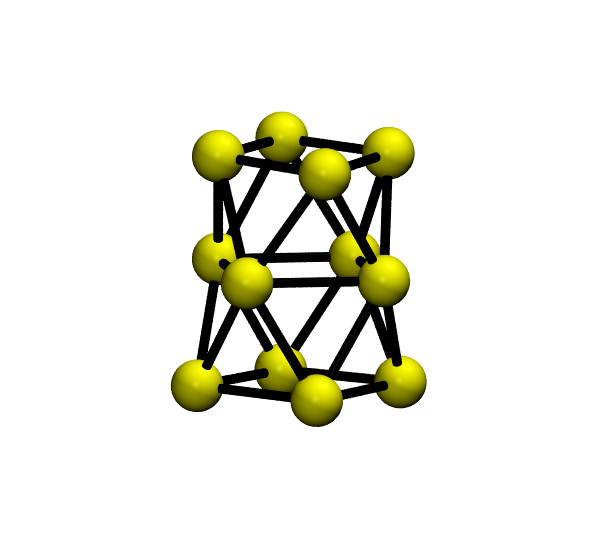
\includegraphics[width=0.25\textwidth]{golddual/anions/Au12.png}}
	\subfloat[14:1 ]{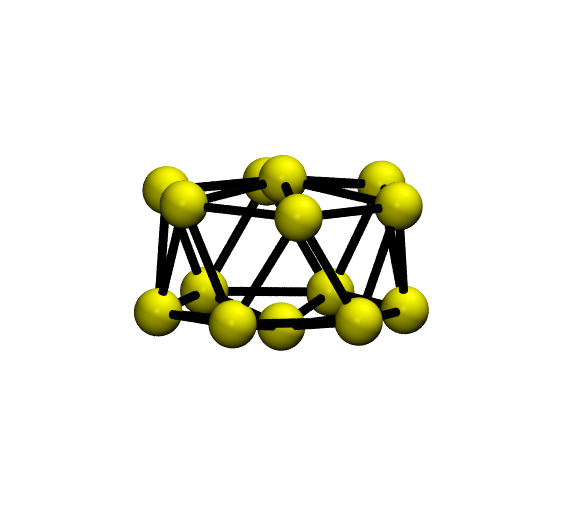
\includegraphics[width=0.25\textwidth]{golddual/anions/Au14.png}}
	\subfloat[15:1 ]{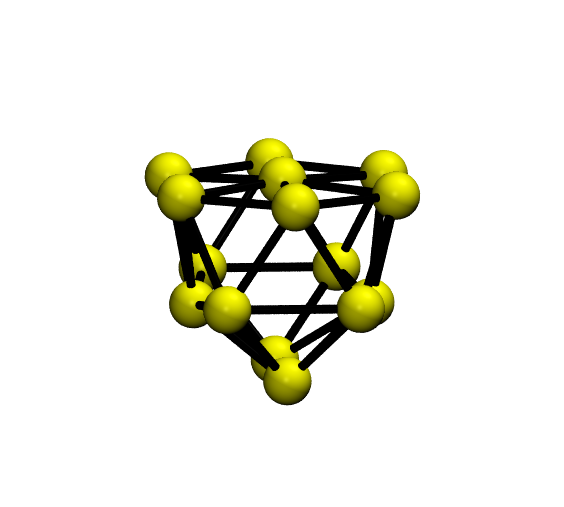
\includegraphics[width=0.25\textwidth]{golddual/anions/Au15.png}}
	\subfloat[16:1 ]{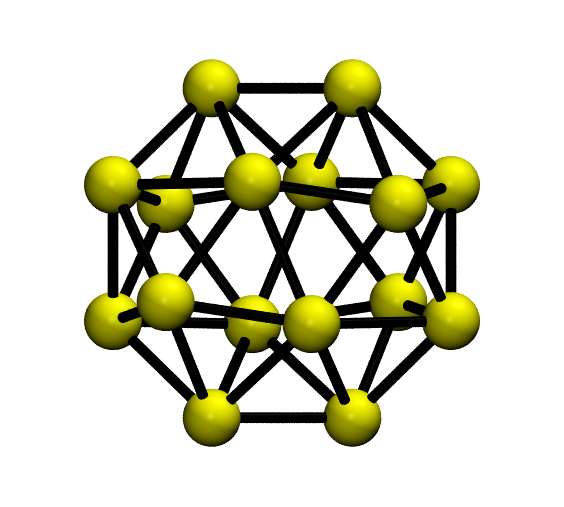
\includegraphics[width=0.25\textwidth]{golddual/anions/Au16-D2.png}}\\
	\subfloat[16:2 ]{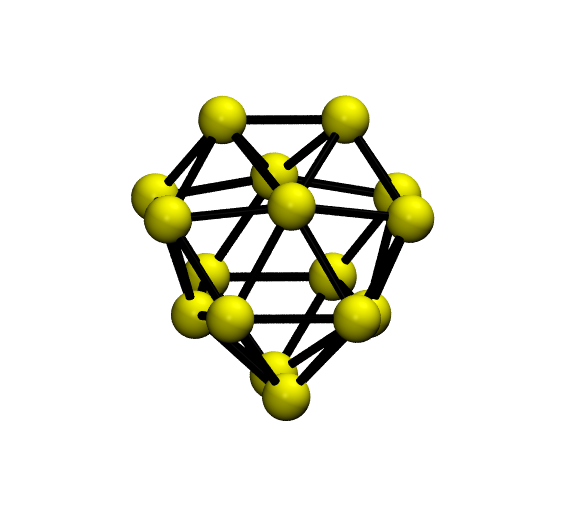
\includegraphics[width=0.25\textwidth]{golddual/anions/Au16-Td.png}}
	\subfloat[17:1 ]{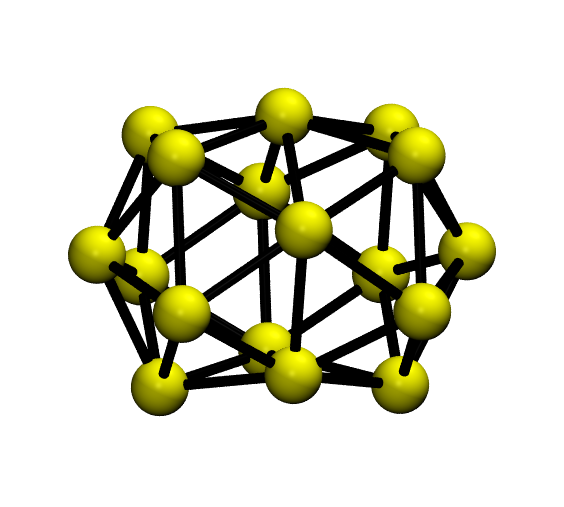
\includegraphics[width=0.25\textwidth]{golddual/anions/Au17-D5h.png}}
	\subfloat[17:2 ]{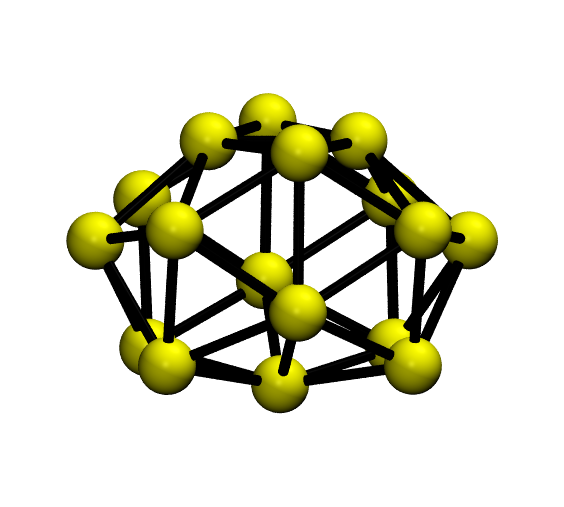
\includegraphics[width=0.25\textwidth]{golddual/anions/Au17-C2v-1.png}}
	\subfloat[17:3 ]{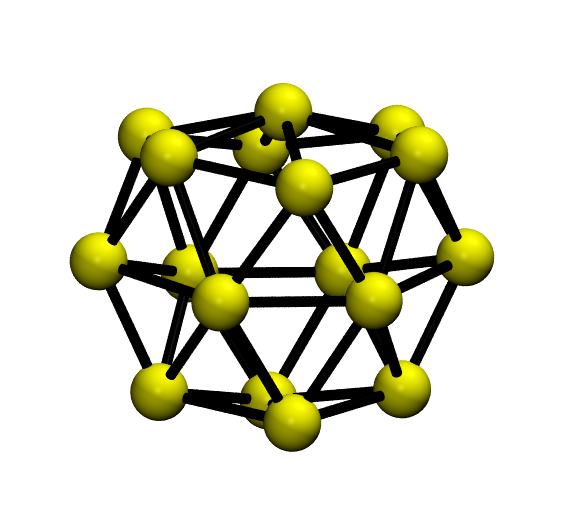
\includegraphics[width=0.25\textwidth]{golddual/anions/Au17-C2v-2.png}}\\
	\subfloat[18:1 ]{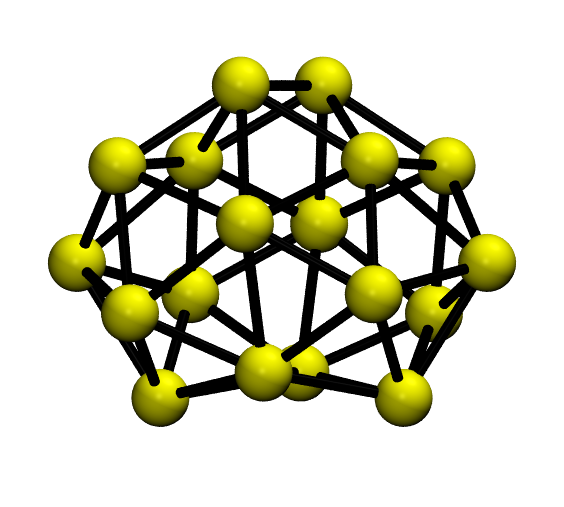
\includegraphics[width=0.25\textwidth]{golddual/anions/Au18-C2-1.png}}
	\subfloat[18:2 ]{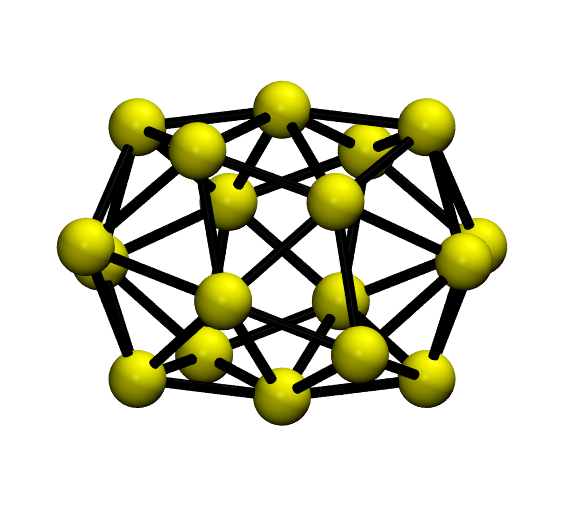
\includegraphics[width=0.25\textwidth]{golddual/anions/Au18-D2.png}}
	\subfloat[18:3 ]{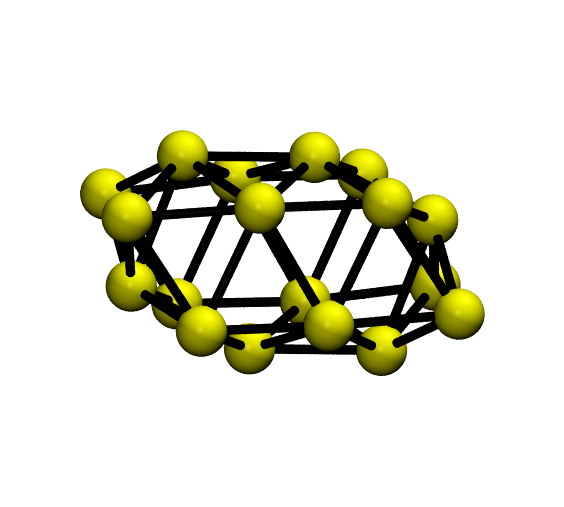
\includegraphics[width=0.25\textwidth]{golddual/anions/Au18-D3d.png}}
	\subfloat[18:4 ]{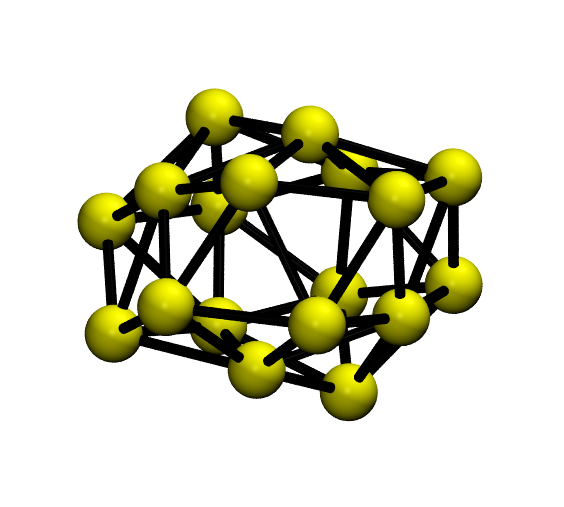
\includegraphics[width=0.25\textwidth]{golddual/anions/Au18-C2-2.png}}\\
	\subfloat[18:5 ]{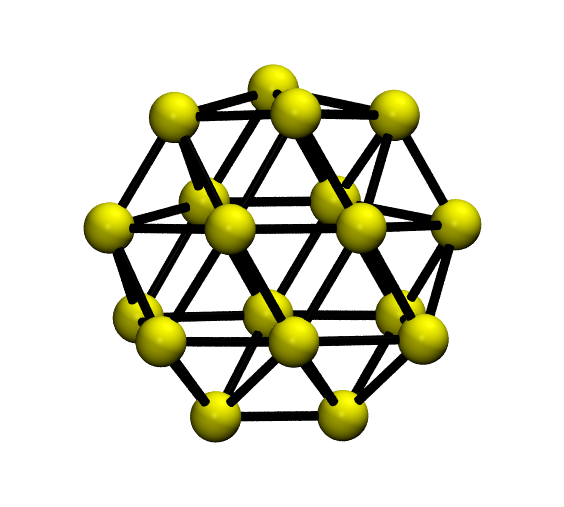
\includegraphics[width=0.25\textwidth]{golddual/anions/Au18-D3h.png}}
	\subfloat[18:6 ]{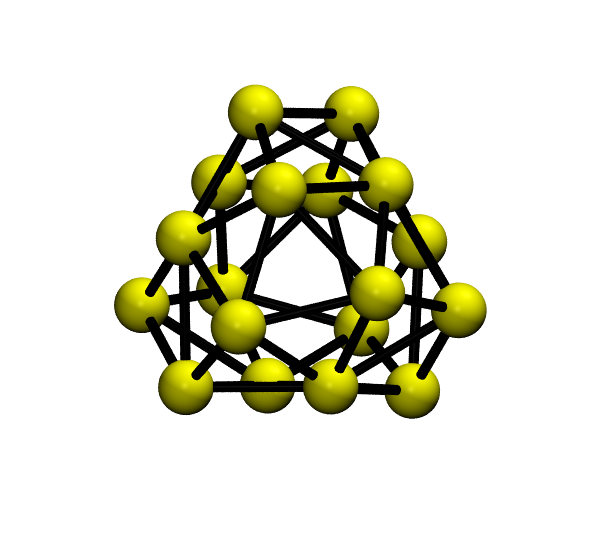
\includegraphics[width=0.25\textwidth]{golddual/anions/Au18-D3.png}}
	\subfloat[19:1 ]{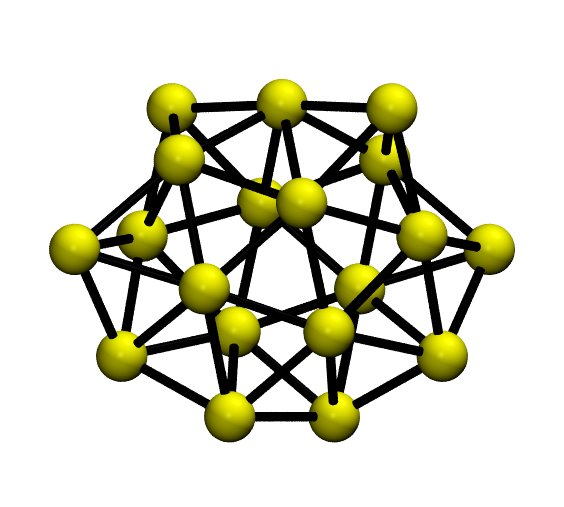
\includegraphics[width=0.25\textwidth]{golddual/anions/Au19-C2-1.png}}
	\subfloat[19:2 ]{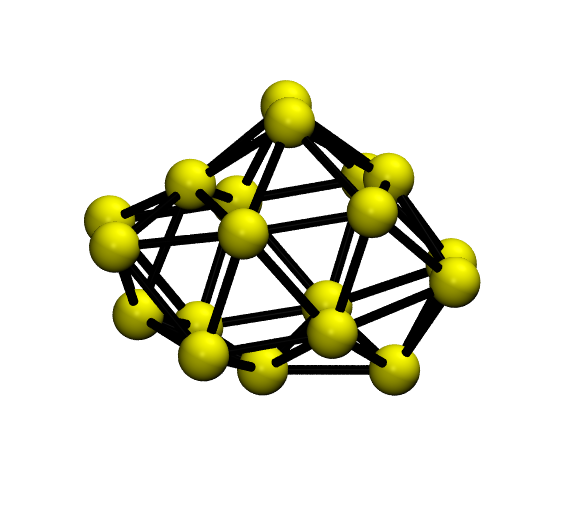
\includegraphics[width=0.25\textwidth]{golddual/anions/Au19-Cs-1.png}}\\
	\subfloat[19:3 ]{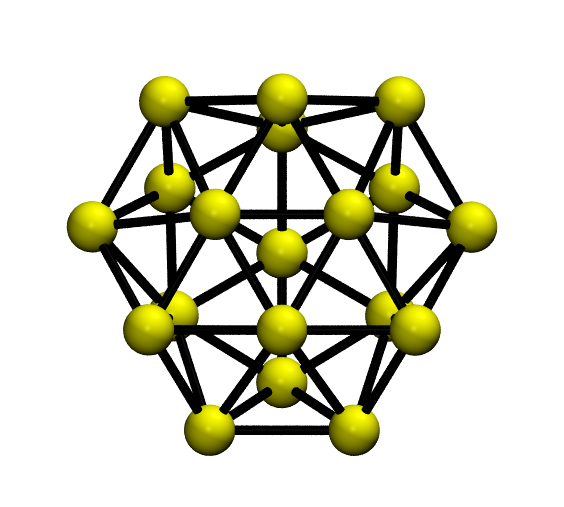
\includegraphics[width=0.25\textwidth]{golddual/anions/Au19-Cs-2.png}}
	\subfloat[19:4 ]{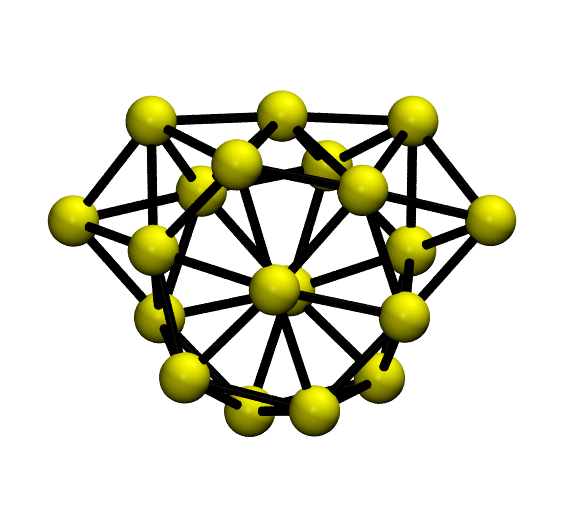
\includegraphics[width=0.25\textwidth]{golddual/anions/Au19-C2-2.png}}
	\subfloat[19:5 ]{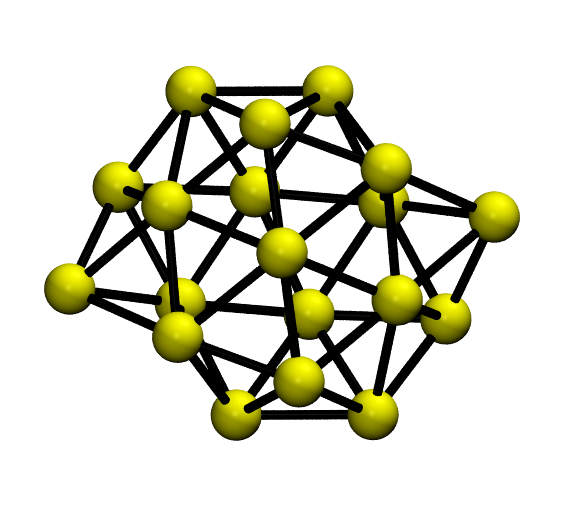
\includegraphics[width=0.25\textwidth]{golddual/anions/Au19-C2-3.png}}
	\subfloat[19:6 ]{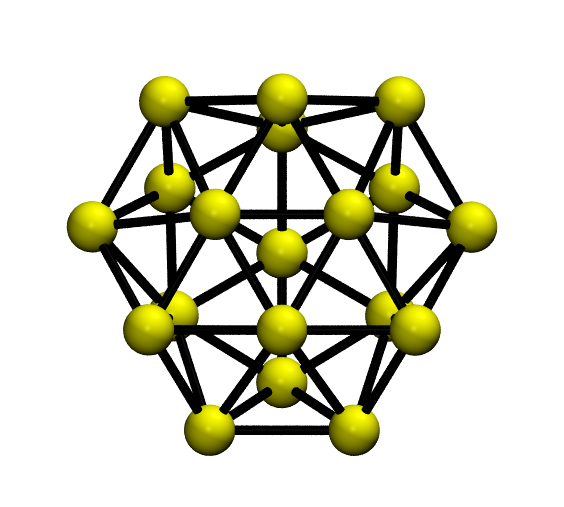
\includegraphics[width=0.25\textwidth]{golddual/anions/Au19-C3v.png}}
	\caption{Structures of anionic gold clusters (Au$_{12}^-$ to Au$_{19}^-$).}
	\label{fig:Au1219-}
\end{center}
\end{figure}
\begin{figure}
	\begin{center}
	\subfloat[20:1 ]{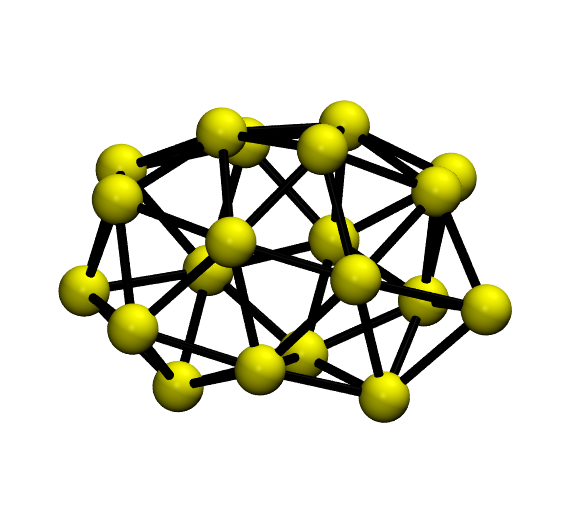
\includegraphics[width=0.25\textwidth]{golddual/anions/Au20-C2-1.png}}
	\subfloat[20:2 ]{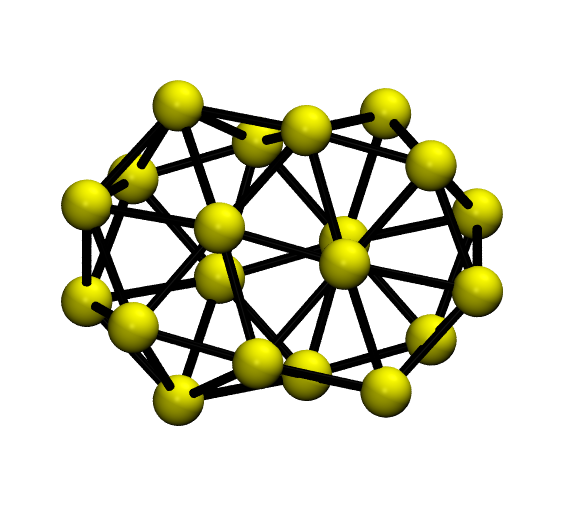
\includegraphics[width=0.25\textwidth]{golddual/anions/Au20-D2-1.png}}
	\subfloat[20:3 ]{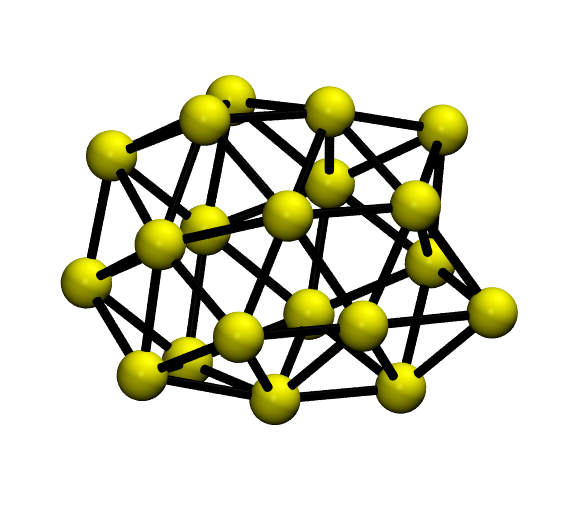
\includegraphics[width=0.25\textwidth]{golddual/anions/Au20-C1-1.png}}
	\subfloat[20:4 ]{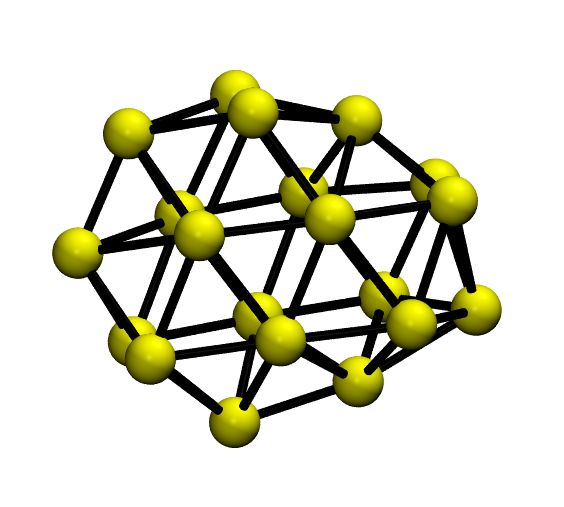
\includegraphics[width=0.25\textwidth]{golddual/anions/Au20-Cs-1.png}}\\
	\subfloat[20:5 ]{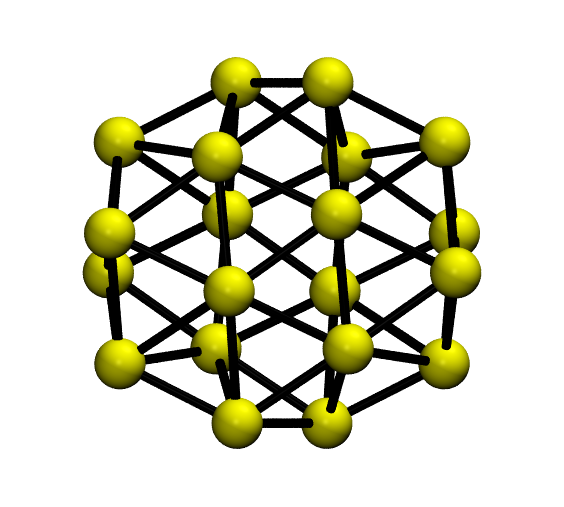
\includegraphics[width=0.25\textwidth]{golddual/anions/Au20-D2-2.png}}
	\subfloat[20:6 ]{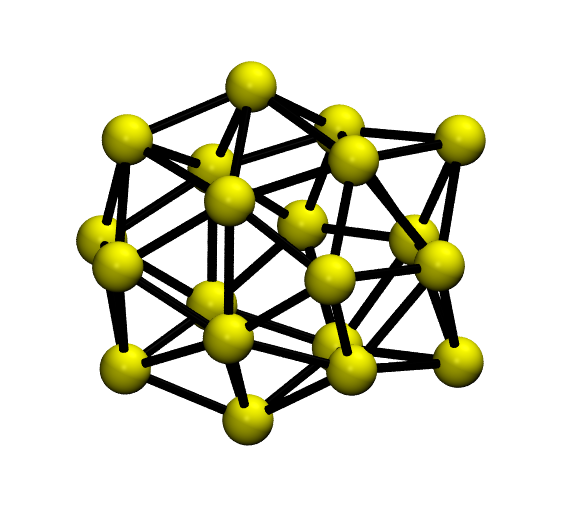
\includegraphics[width=0.25\textwidth]{golddual/anions/Au20-D2d-1.png}}
	\subfloat[20:7 ]{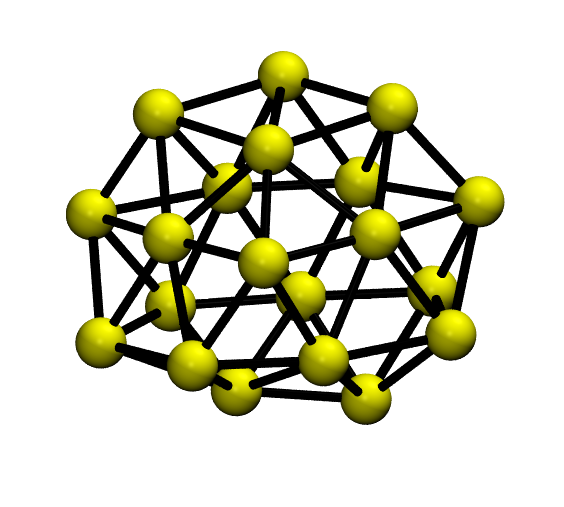
\includegraphics[width=0.25\textwidth]{golddual/anions/Au20-C1-2.png}}
	\subfloat[20:8 ]{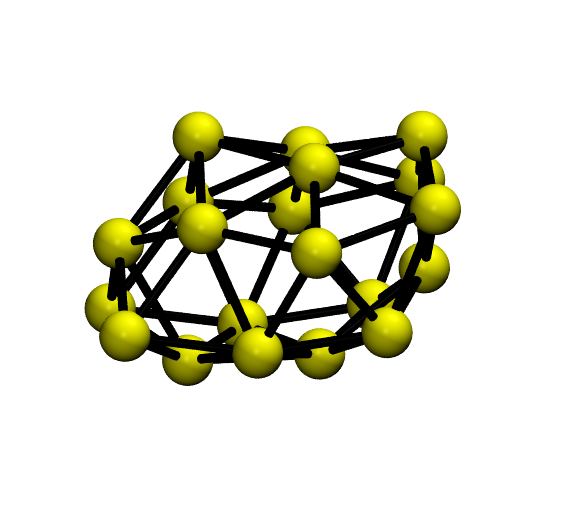
\includegraphics[width=0.25\textwidth]{golddual/anions/Au20-Cs-2.png}}\\
	\subfloat[20:9 ]{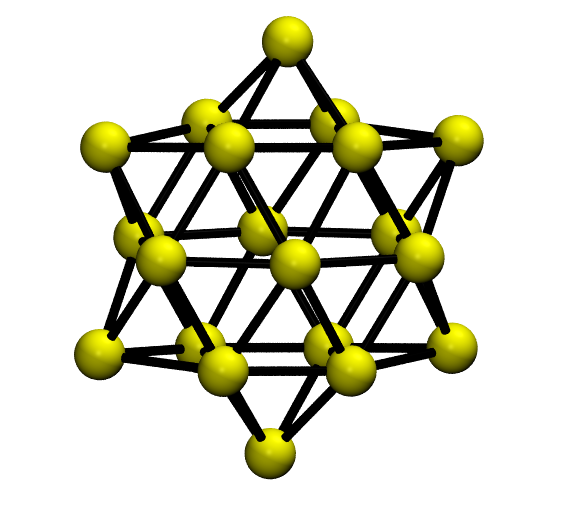
\includegraphics[width=0.25\textwidth]{golddual/anions/Au20-C2v.png}}
	\subfloat[20:10]{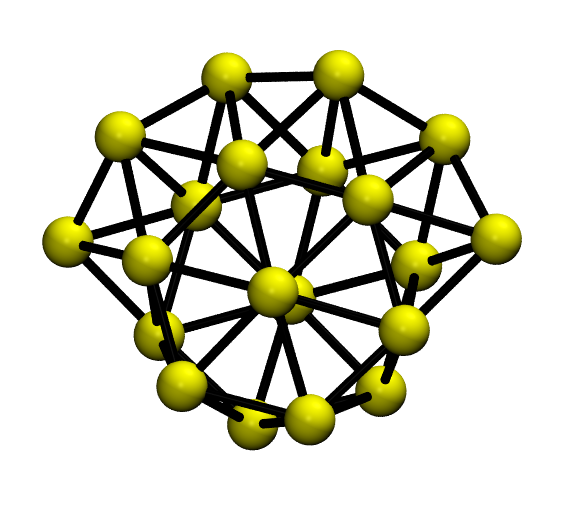
\includegraphics[width=0.25\textwidth]{golddual/anions/Au20-C2-2.png}}
	\subfloat[20:11]{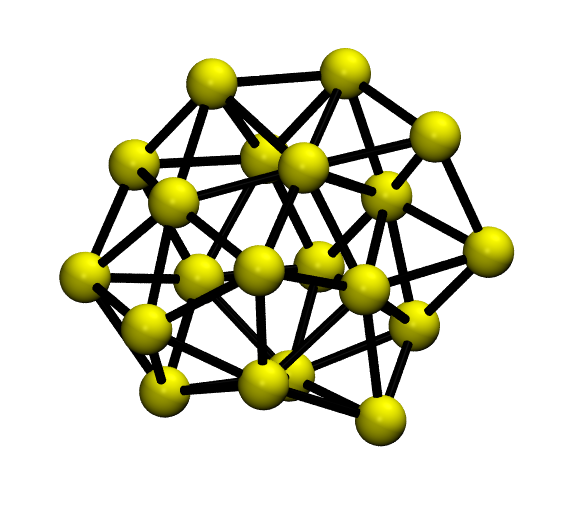
\includegraphics[width=0.25\textwidth]{golddual/anions/Au20-C2-3.png}}
	\subfloat[20:12]{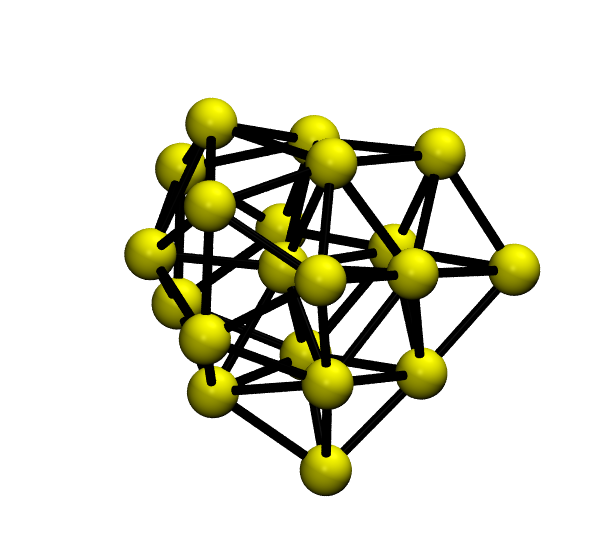
\includegraphics[width=0.25\textwidth]{golddual/anions/Au20-C2-4.png}}\\
	\subfloat[20:13]{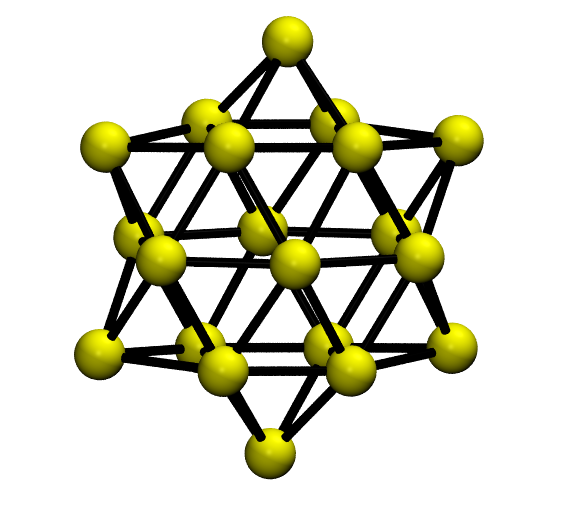
\includegraphics[width=0.25\textwidth]{golddual/anions/Au20-D3h.png}}
	\subfloat[20:14]{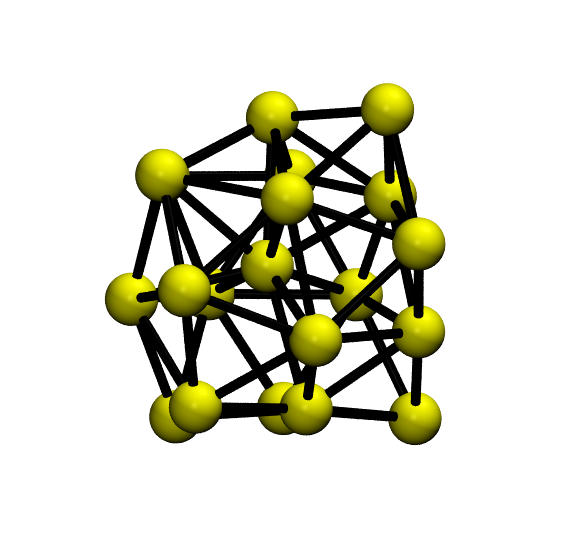
\includegraphics[width=0.25\textwidth]{golddual/anions/Au20-D2d-2.png}}
	\subfloat[20:15]{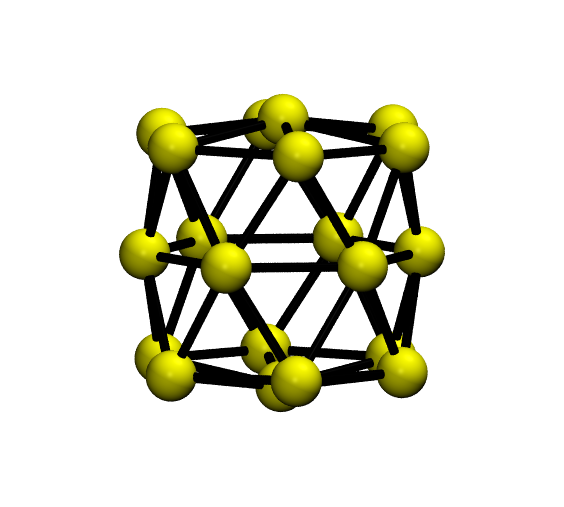
\includegraphics[width=0.25\textwidth]{golddual/anions/Au20-D6h.png}}
	\caption{Structures of anionic gold clusters (Au$_{20}^-$).}
	\label{fig:Au20-}
\end{center}
\end{figure} 

\begin{figure}[htbp]
\begin{center}
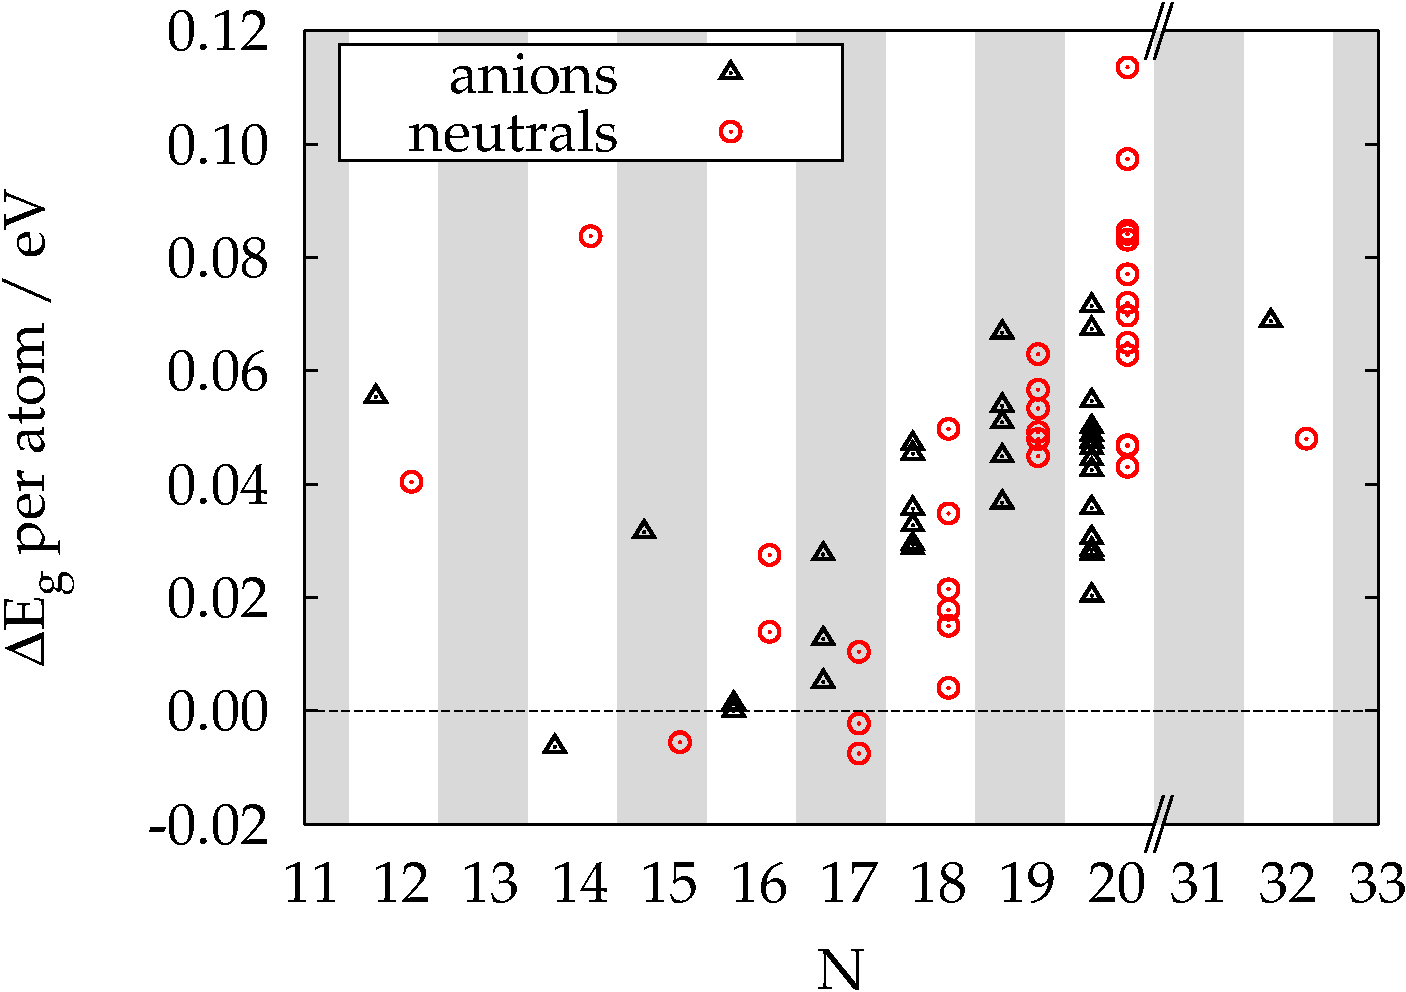
\includegraphics[width=10cm]{golddual/energies.pdf}
\caption{Relative energies for the investigated dual fullerene clusters.
Energy differences compared to the most stable compact cluster (per atom) are given in eV.}
\label{fig:AunMinus2}
\end{center}
\end{figure}

\begin{figure}\centering
	\begin{tabular}{lp{3cm}|p{3cm}}\toprule
		isomer  & \multicolumn{1}{c}{neutral} & \multicolumn{1}{c}{anion} \\ \midrule
		12:1    & \cellcolor{myorange}        & \cellcolor{myorange}      \\
		14:1    & \cellcolor{mygreen}         & \cellcolor{mygreen}       \\
		15:1    & \cellcolor{mygreen}         & \cellcolor{mygreen}       \\
		16:1    & \cellcolor{mygreen}         & \cellcolor{mygreen}       \\
		16:2    & \cellcolor{mygreen}         & \cellcolor{mygreen}       \\
		17:1    & \cellcolor{myorange}        & \cellcolor{mygreen}       \\
		17:2    & \cellcolor{mygreen}         & \cellcolor{mygreen}       \\
		17:3    & \cellcolor{mygreen}         & \cellcolor{mygreen}       \\
		18:1    & \cellcolor{mygreen}         & \cellcolor{mygreen}       \\
		18:2    & \cellcolor{mygreen}         & \cellcolor{mygreen}       \\
		18:3    & \cellcolor{mygreen}         & \cellcolor{myorange}      \\
		18:4    & \cellcolor{mygreen}         & \cellcolor{mygreen}       \\
		18:5    & \cellcolor{mygreen}         & \cellcolor{mygreen}       \\
		18:6    & \cellcolor{mygreen}         & \cellcolor{mygreen}       \\
		19:1    & \cellcolor{mygreen}         & \cellcolor{myorange}      \\
		19:2    & \cellcolor{mygreen}         & \cellcolor{myorange}      \\
		19:3    & \cellcolor{mygreen}         & \cellcolor{mygreen}       \\
		19:4    & \cellcolor{mygreen}         & \cellcolor{myorange}      \\
		19:5    & \cellcolor{mygreen}         & \cellcolor{myorange}      \\
		19:6    & \cellcolor{mygreen}         & \cellcolor{mygreen}       \\
		20:1    & \cellcolor{myorange}        & \cellcolor{myorange}      \\
		20:2    & \cellcolor{mygreen}         & \cellcolor{mygreen}       \\
		20:3    & \cellcolor{myorange}        & \cellcolor{myorange}      \\
		20:4    & \cellcolor{mygreen}         & \cellcolor{mygreen}       \\
		20:5    & \cellcolor{mygreen}         & \cellcolor{mygreen}       \\
		20:6    & \cellcolor{myorange}        & \cellcolor{myorange}      \\
		20:7    & \cellcolor{myorange}        & \cellcolor{mygreen}       \\
		20:8    & \cellcolor{myorange}        & \cellcolor{myorange}      \\
		20:9    & \cellcolor{myorange}        & \cellcolor{myorange}      \\
		20:10   & \cellcolor{myorange}        & \cellcolor{myorange}      \\
		20:11   & \cellcolor{myorange}        & \cellcolor{myorange}      \\
		20:12   & \cellcolor{red}             & \cellcolor{red}           \\
		20:13   & \cellcolor{myorange}        & \cellcolor{myorange}      \\
		20:14   & \cellcolor{mygreen}         & \cellcolor{red}           \\
		20:15   & \cellcolor{myorange}        & \cellcolor{mygreen}       \\
		32:1082 & \cellcolor{mygreen}         & \cellcolor{mygreen}       \\ \bottomrule
	\end{tabular}
	\caption{Overview of PBE-D3 optimization results for the dual fullerene structures. 
	Green: dual fullerene structure, orange: hollow structure, red: non-hollow structure.}
	\label{fig:optOverview}
\end{figure}

We can sort out the optimized gold clusters according to whether they can
be derived from a dual fullerene structure or not, or more generally from a cubic polyhedral
graph. In this case 
we can simplify Euler's polyhedral formula, which upon dualization (i.e. swapping the role of vertices with faces)
gives a triangulation of a sphere obeying the formula,
\begin{equation}
\label{eq3valent} 
\Gamma=\sum_{n=3}(6-n)N_n = 12
\end{equation}
where $N_m$ denotes
the number of $m$-valent vertices. Any deviation from $\Gamma$=12 implies that the
polyhedron is not a triangulation of a sphere. For dual fullerenes we only allow for
$N_5$=12 and $N_6=0$ or $N_6>1$. Hence we have to look for a complete
triangulation and 12 vertices of degree 5 to obtain a dual fullerene
structure (also called a geodesic dome).

Tables~\ref{tab:neutral} and \ref{tab:anion} show vertex counts as well as
results from equation~(\ref{eq3valent}) for the neutral and anionic clusters,
respectively. Considering only the topological parameter $\Gamma$ it is clear that most of the optimized
structures can be derived from a dual planar cubic graph and therefore only
consist of triangles. The few notable exceptions are the isomers 12:1 and 20:12 for
both the anionic and neutral structure. The ideal icosahedral structure for the
Au$_{12}$ cluster is not stable under the present level of theory, and the optimized
structure does not correspond to a triangulation of a sphere. However, it has
already been shown that this cage can
be stabilized by inserting a transition metal (e.g. tungsten) atom into the central position
of the icosahedron such that the 10 valence electron rule is
fulfilled.\autocite{Pyykko_IcosahedralWAu12Predicted_2002,Autschbach_PropertiesWAu12_2004} Addition stabilization of such
an endohedral gold cluster can be achieved by attaching ligands to the surface
of the cluster.\autocite{Laupp-1994} Structure 20:12 converges
towards a more compact cluster with an 8-fold coordinated gold atom in the centre
for both the anionic and the neutral cluster.  

Figure~\ref{fig:optOverview} gives an overview over all optimized structures. 
A green field marks a dual fullerene structure with
exactly 12 vertices of degree five and the remaining vertices being of degree
six. These are also the structures used in Figure~\ref{fig:cohesiveenergies2}
and they are more abundant for clusters of size 14 to 19 atoms. Structures with an
orange mark do not fulfill the requirement of being a dual fullerene as they contain
vertices of degree 4. However,
they are still hollow gold cages and, as mentioned before, show a value of
$\Gamma$=12. These structures can be rather similar to the initial dual fullerene
structures obtained from a force-field optimization of the corresponding carbon cage,
and are usually a result of a flattening towards a more oblate geometry. 
Most of the clusters shown here preserve their hollow cage structure 
with only few clusters optimizing into more stable compact structures. These
are marked as red in Figure~\ref{fig:optOverview}.


As illustrated by the distortion parameter $D$(F) in Tables~\ref{tab:neutral} and
\ref{tab:anion}, carbon fullerenes try to adopt ``spherical'' shapes if permitted
by the distribution of pentagons. This is especially the case for $I_h$-C$_{20}$
and $I_h$-C$_{60}$ with a distortion parameter of exactly zero (i.e. all atoms lie on a sphere). 
In contrast, the golden dual fullerene structures have much larger distortion parameters $D$(GDF) than their
carbon equivalent and are therefore less spheroidal. The golden dual fullerenes usually distort
into less symmetric structures, for example into oblate structures as mentioned above.

Figure~\ref{fig:AunMinus2} shows the relative energies $\Delta E_g$ per atom compared to
the most stable compact arrangement for all optimized hollow gold clusters. 
It is immediately apparent, that the most stable dual fullerene
structures can be found in the region of 14 to 18 atoms. Some clusters in this
region even exceed the stability of formerly proposed global minimum
structures. For example, for Au$_{16}^-$ the global minimum has been proposed before to be the tetrahedral hollow
cluster\autocite{Schooss_Determiningsizedependentstructure_2010,Lechtken_Structuredeterminationgold_2009} which is the dual of the tetrahedral
C$_{28}$ isomer as observed experimentally in photoelectron spectra.\autocite{Bulusu_Evidencehollowgolden_2006}
We should mention, that Chen et al. have found the
tetrahedral structure to lie 0.22~eV above a sheet-like
structure.\autocite{Chen_Structuresneutralanionic_2010} However, our results contradict these findings as
the planar structure is predicted to be 0.939~eV higher in energy. 
Here we point out that according to our calculations the D$_2$ symmetric isomer 16:1 lies
only 0.02~eV above the tetrahedral structure.
Therefore, it should also be possible to observe this isomer by experimental methods.

Possible Au$_{32}$ structures have been investigated intensively by Jalbout et
al.\autocite{Jalbout_LowSymmetryStructuresAu_2008} We compare our results to the most stable isomers found
in their work (Table~\ref{tab:Aun}). For both neutral and anionic clusters,
isomer 10 in their work (see ref.\autocite{Jalbout_LowSymmetryStructuresAu_2008} for details) turns out to be 
the most stable compact geometry and the icosahedral hollow
structure 32:1082 is less stable in both cases, i.e. for the neutral and anionic cluster.
We also include the $C_{3v}$ compact structure in Table~\ref{tab:Aun} not
investigated before, which is derived from the ideal Au$_{35}$ tetrahedron by removing
three of the corner atoms in the tetrahedron and can be seen as a cut-out of the
fcc bulk structure. This cluster is also very stable compared to the other structures
proposed by Jalbout et al. We also mention that the Au$_{32}$ hollow cage distorts from an ideal
icosahedral symmetry into a $D_{2h}$ arrangement, which is reflected in the distortion parameter
$D$(Au$_{32}$)=10.4, which however is rather small. Au$_{32}$ can therefore be seen as pseudo-spherical.
  

\subsection{Convergence towards the infinite structure}

The neutral gold clusters and their property convergence towards the bulk has
already been discussed in one of our previous papers.\autocite{Assadollahzadeh_systematicsearchminimum_2009}
Increasing the size of non-hollow compact clusters lowers the cohesive energy until the
clusters are large enough to be a valid representation of the bulk gold structure.
This can be seen in Figure~\ref{fig:cohesiveenergies1}, where a clear linear
correlation between cluster size and the cohesive energy is depicted.

\begin{figure}\centering
	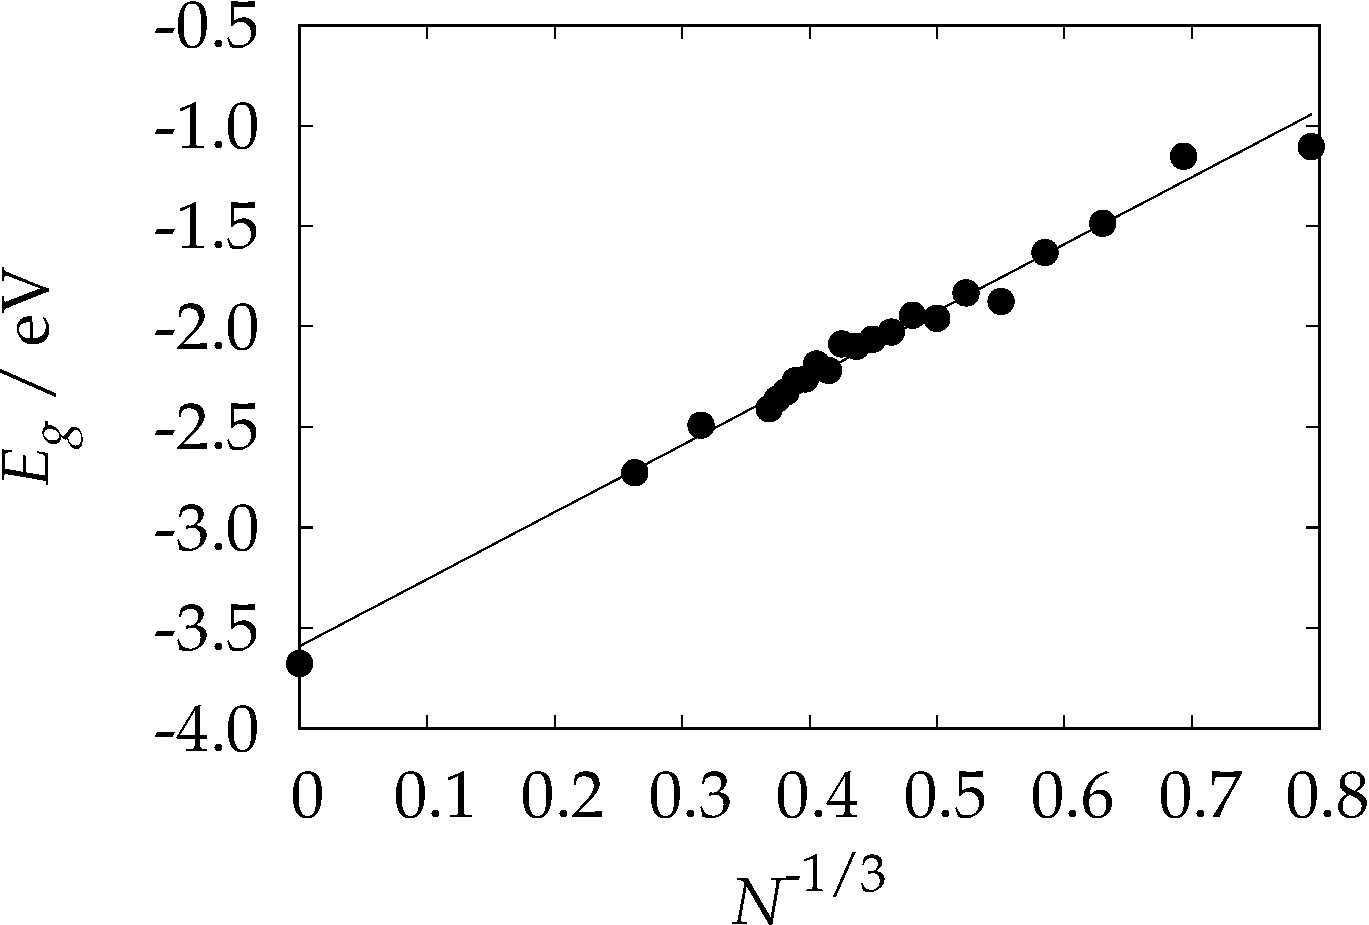
\includegraphics[width=10cm]{golddual/cohesive.pdf}
	\caption{Cohesive energies for the compact gold clusters with cluster size $N$ and convergence toward the bulk fcc structure.}
	\label{fig:cohesiveenergies1}
\end{figure}

Hollow gold clusters can be created by wrapping a cutout from a (111) gold 2D sheet
around a sphere introducing 12 vertices of degree 5 to satisfy Euler's theorem. 
Therefore, an infinitely large 2D gold sheet represents a
golden dual fullerene cage with an infinite sphere radius. As the cohesive energy
of the compact structures converges towards the bulk cohesive energy,
the cohesive energy of the 2D gold sheet should represent the infinite limit for the dual
golden fullerene structures. This is indeed the case and is depicted in Figure~\ref{fig:cohesiveenergies2}
using a $N^{-1}$ scaling law analog to the one used for fullerenes (for details see ref.\autocite{Wirz_smallfullerenesgraphene_2015}). 

\begin{figure}\centering
	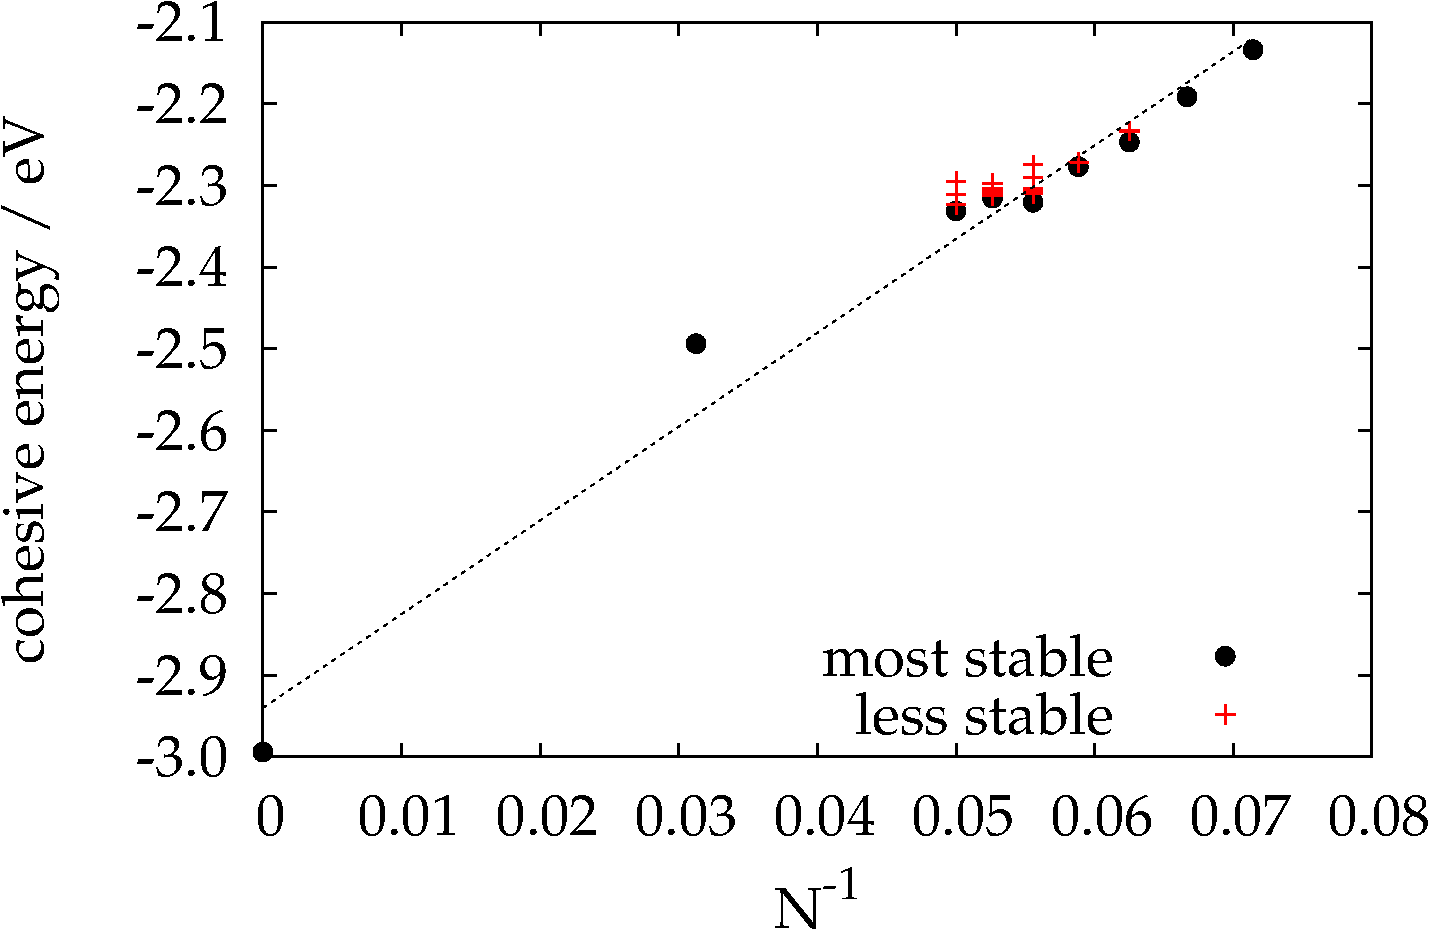
\includegraphics[width=10cm]{golddual/cohesive2.pdf}
	\caption{Cohesive energies for the hollow gold clusters with cluster size $N$ and convergence toward the (111) gold sheet.}
	\label{fig:cohesiveenergies2}
\end{figure}

An interesting result here is the difference between the cohesive energy of the
bulk fcc structure compared to the (111) 2D sheet. Creating the bulk structure
from stacking (111) sheets only accounts for $\sim$0.68~eV of the total
cohesive energy of the bulk which is 3.81 eV.\autocite{takeuchi_first-principles_1989} This implies
that most of the cohesive energy of bulk gold originates from the (111) sheet,
which is therefore exceptionally stable and can be seen as a reason for the
preferred planar arrangement of many small gold clusters.  As pointed out by
Takeuchi et al, relativistic effects increase the cohesive energy of bulk gold
by 1.5 eV.\autocite{takeuchi_first-principles_1989} A similar large relativistic effect is expected
for the (111) sheet of gold.

\subsection{Simulation of photoelectron spectra}

Photoelectron spectra of several golden cages dual fullerenes have been
determined experimentally and simulated by theoretical methods by Bulusu et
al.\autocite{Bulusu_Evidencehollowgolden_2006} Before we discuss our results we need to consider
spin-orbit effects as substantial 5d-mixing into the 6s orbitals of gold occurs
in such clusters. Figure \ref{fig:photoSOAu17} shows a comparison of simulated
photoelectron spectra of the three golden dual fullerene isomers of
Au$_{17}^-$. The results clearly shows that spin-orbit effects can be
neglected in this energy range.

\begin{figure}\centering
	\subfloat[]{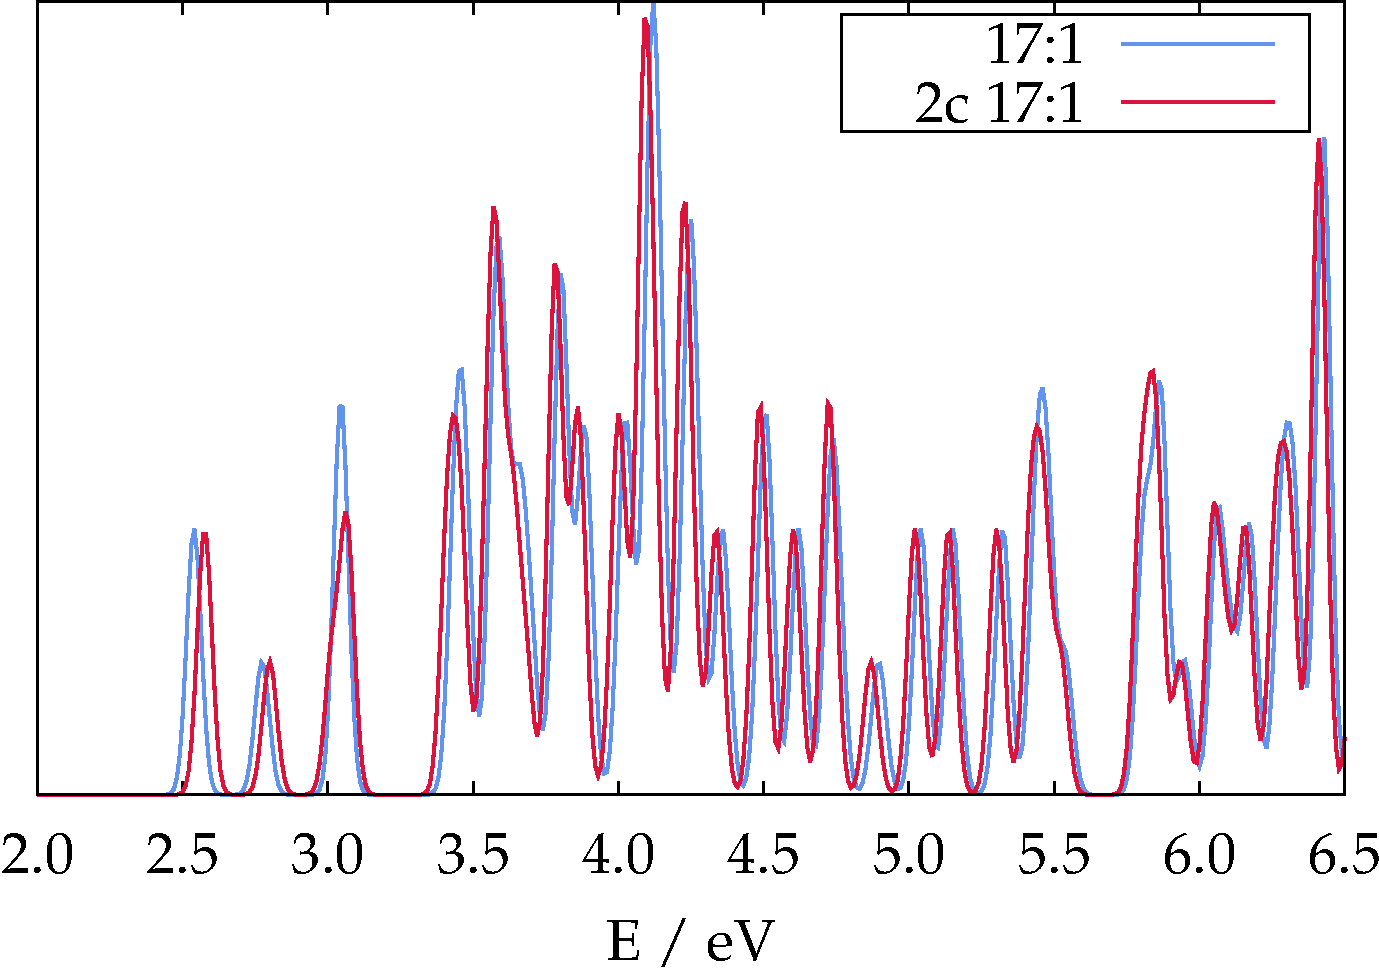
\includegraphics[width=.49\textwidth]{golddual/photo/Au17/turbo/rel-nonrel/photo1.pdf}}\hfill
	\subfloat[]{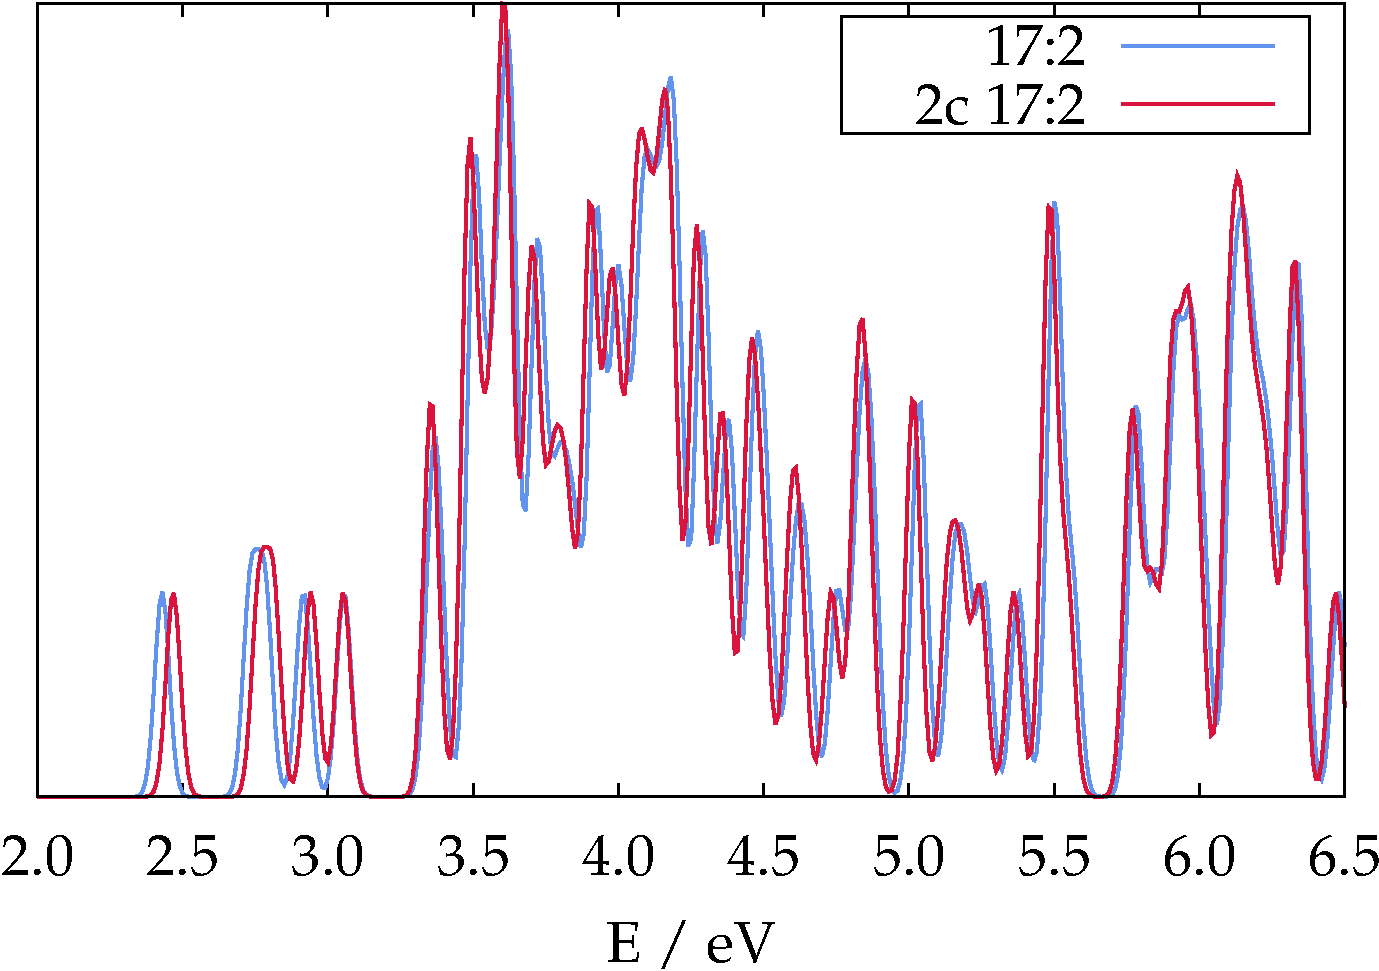
\includegraphics[width=.49\textwidth]{golddual/photo/Au17/turbo/rel-nonrel/photo2.pdf}}\\
	\subfloat[]{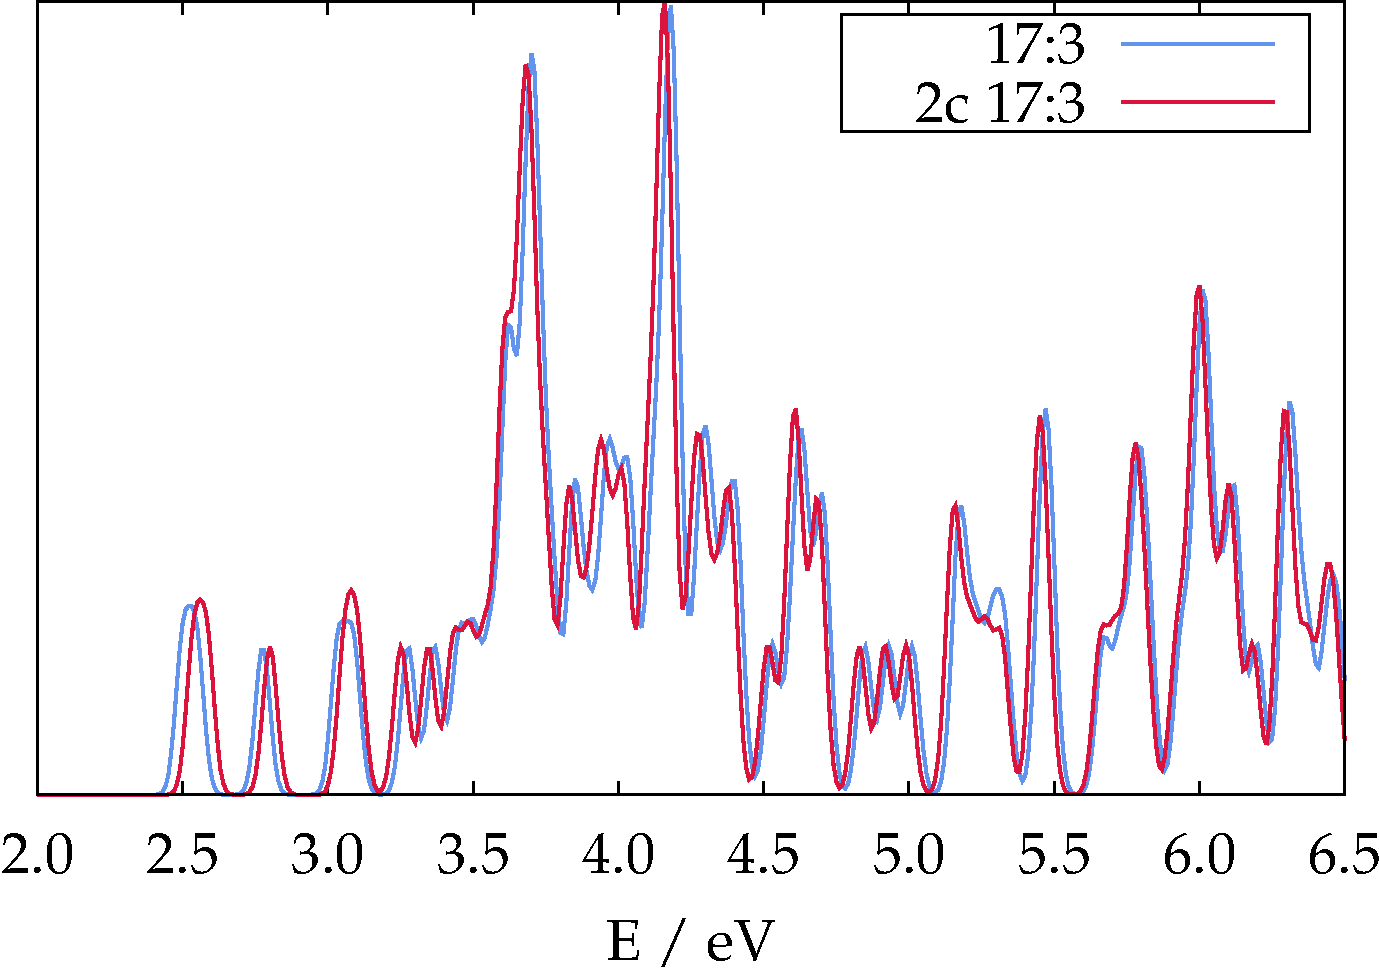
\includegraphics[width=.49\textwidth]{golddual/photo/Au17/turbo/rel-nonrel/photo3.pdf}}
	\caption{Comparison of simulated photoelectron spectra of the three dual fullerene isomers of Au$_{17}^-$ with (2c) and without spin-orbit coupling.} 
	\label{fig:photoSOAu17}
\end{figure}

\begin{figure}[htbp]
\begin{center}
    \subfloat[]{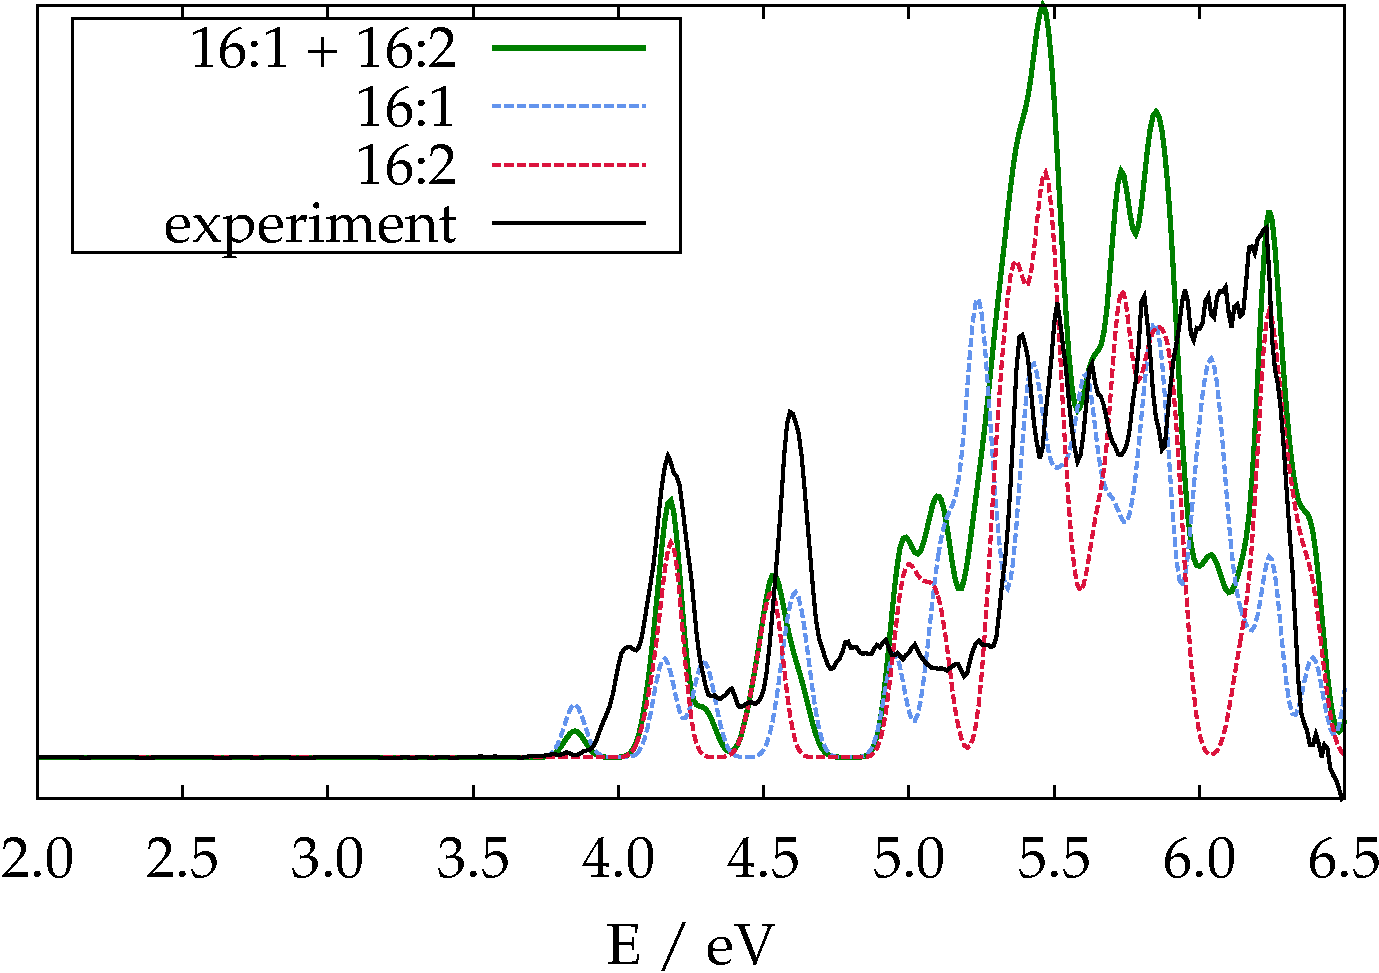
\includegraphics[width=.49\textwidth]{golddual/photo/Au16/turbo/photo1.pdf}}\hfill
    \subfloat[]{\includegraphics[width=.49\textwidth]{golddual/photo/Au17/turbo/compare/compare.pdf}}\\
    \subfloat[]{\includegraphics[width=.49\textwidth]{golddual/photo/Au18/turbo/nonrel/compare.pdf}}
\caption{Simulated photoelectron spectra for the negatively charged hollow gold clusters 
(shifted to the experimental threshold energy). a) Top: The two possible
dual fullerene isomers of Au$_{16}^-$ . The green curve shows a combination of the $D_2$ and $T_d$ spectra with a ratio of 1:1.; b) Middle: The three possible dual fullerene isomers of Au$_{17}^-$; c) Bottom:
The six possible dual fullerene isomers of Au$_{18}^-$ (shifted to the experimental threshold energy).}
  \label{fig:photo_Au16}
\end{center}
\end{figure}

Bulusu et al. considered only the $Au_{16}^-$ $T_d$ structure. From our data
there is reason to believe that the other possible isomer 16:1 is also present
in the measured spectrum. Figure~\ref{fig:photo_Au16} shows our simulation
results for the isomers 16:1 and 16:2 and a simulation for a mixture of both
compounds with a ratio of 1:1 as the energy of both isomers are comparable. 
Looking at the experimental data a shoulder can
be identified in the first peak. We can reproduce this feature by shifting the
spectra for 16:1 and 16:2 according to the corresponding vertical ionization
potential, superimposing both spectra and shift the result by 0.18~eV to better
fit the experimental data as pictured in Figure~\ref{fig:photo_Au16}. This
indicates that the second hollow cage isomer has also been produced.
Further evidence for this could be the experimental peak at 5.51~eV. The
simulated spectrum for the tetrahedral cluster shows a dip at this energy,
while the D$_2$ structure has a clear intensity maximum. 

Figure~\ref{fig:photo_Au16} shows the simulated spectra for the three possible
dual fullerene isomers for Au$_{17}^-$. The spectra have been shifted according
to the vertical ionization potential of the negatively charged clusters. The most
stable structures are 17:2 (red) and 17:3 (green) of which 17:2 fits reasonably
well for the first 4 peaks. The peak at 4.73~eV could be accounted to the 17:3
isomer which is identical to Bulusu et al.'s C$_{2v}$ symmetric structure.

From the relative energies in Figure~\ref{fig:AunMinus2} it is clear that
anionic dual fullerene structures start to become rather unstable for $N$=18.
Therefore, compact clusters might dominate the experimental spectrum.
Figure~\ref{fig:photo_Au16} shows our calculated spectra in comparison with the
experimental data. The calculated spectra have been first shifted to the
corresponding vertical ionization potential and subsequently shifted by 0.25~eV
to better fit the experimental data. The most stable dual fullerene clusters are
18:1, 18:4 and 18:5. 18:1 and 18:5 could be responsible for the second peak in
the experimental data at 3.63~eV, while 18:4 agrees with the first peak. The
signal at 3.97~eV could be and an indication that isomer 18:3 was produced as it is
the only structure that shows a peak in that area, although it is the least
stable of the hollow structures.

Finally, for future experiments we include our simulated photoelectron spectrum
for Au$_{32}^-$ which is shown in Figure~\ref{fig:photo_Au32}. 

\begin{figure}[htbp]
\begin{center}
\includegraphics[width=.8\textwidth]{golddual/photo/Au32/nonrel/compare.pdf}
\caption{Simulated photoelectron spectra for 32:1812 isomer of Au$_{32}^-$.}
  \label{fig:photo_Au32}
\end{center}
\end{figure}


\subsection{Summary}

We found an interesting topological relationship between fullerenes and the
cage-like gold clusters resulting in a triangulation of a sphere with vertices
of degrees 5 and 6 fulfilling Euler's polyhedral formula. Because of this
isomorphism between the two structures by dualization, there are as many golden
fullerene isomers as there are different fullerene structures. In the same way
we relate gold nanotubes to carbon nanotubes and halma transforms of C$_{20}$
to the shells of a Mackay icosahedron. We investigated the stability of these
golden fullerenes. While they perhaps may not compete in energy with the more
compact gold clusters at larger cluster size, the smaller cage structures are
stable as observed by photoelectron spectroscopy. Our simulated photoelectron
spectra suggest that more than one golden fullerene isomer was observed. A
natural step in the next direction would be to stabilize such hollow gold
clusters by either endohedral enclosure of gold or other metal atoms or by
attaching appropriate ligands to the outside of the cage.

\chapter[From Sticky-Hard-Sphere to Lennard-Jones-Type clusters]{
    From Sticky-Hard-Sphere to Lennard-Jones-Type clusters\footnote{This
    chapter is partly composed of sections previously published in the article
    ``From sticky-hard-sphere to Lennard-Jones-type
    clusters''\autocite{Trombach_stickyhardsphereLennardJonestypeclusters_2018}
    and is reproduced with kind permission from the authors and APS
    (\textcopyright 2018 American Physical Society).}
}
\label{sec:fromstickyhardspheretoLJtypeclusters}


%Introduction
\section{Introduction}


The nucleation of atoms and molecules in the gas phase, or liquid, to the solid
state is still an active research
field\autocite{Stillinger_Packingstructurestransitions_1984,
Martin-1996,Wales-1996, Vlieg_atomicscaleunderstandingcrystal_2007, Arkus-2010,
Woodley-2010, Karthika-2016, Holmes-Cerfon_StickySphereClusters_2017}.  Rowland
noted in 1949 that ``The gap between theory and the experimental approaches to
nucleation has been too wide'' and ``the subject [nucleation] is still in the
alchemical stage'' \autocite{Rowland-1949}. More than half a century later,
despite all the advancements made in cluster physics, ``there is still a large
gap between experiment and theory'' as Unwin noted \autocite{Unwin-2007}.

The underlying reason for this rather slow progress is that cluster formation
is a dynamic process, and fully characterizing the corresponding
high-dimensional potential energy landscape is typically an NP-hard problem,
since there are (presumably) exponentially many local minima at any given
temperature and pressure\autocite{Stillinger_Packingstructurestransitions_1984,
Oganov-2006, Massen_Powerlawdistributionsareas_2007, wales10, Oganov-2011,
calvo12, Wales-2015}.  Moreover, phase transitions between different
morphologies as a function of size $N$ usually occur where $N$ is too large for
an accurate quantum-theoretical treatment \autocite{Waal89,
Cleveland_energeticsstructurenickel_1991, vandewaal96a, Doye-1995,
vandeWaalTd00}.  For example, Krainyukova experimentally studied the growth of
argon clusters \autocite{Krainyukova-2012}, and found that small, initially
icosahedral clusters transform into anti-Mackay clusters for $N>2000$, and
finally into the \ac{fcc} or hcp structures at $N>10^5$ atoms, in
qualitative agreement with theoretical predictions using \ac{LJ} type
potentials \autocite{Martin-1996,
Schwerdtfeger_ExtensionLennardJonespotential_2006, Krainyukova-2007}.  The
notorious \textit{rare gas problem} was solved only very recently by accurate
relativistic quantum methods, correctly predicting a slight preference of the
\ac{fcc} over the hcp phase due to phonon dispersion \autocite{Schwerdtfeger-2016}.

Simple models often have to be used to simulate cluster growth and nucleation
\autocite{Johnston-1999, Shibuta_Homogeneousnucleationmicrostructure_2015,
Leitold-2016, Sweatman-2016}.  The simplest model potentials that can be
applied to theoretical studies of atomic cluster formation are ``HCR-SRA''
potentials with isotropic hard-core-like repulsive and short-range-attractive
interactions \autocite{baxter68}.  The simplest HCR-SRA potential is the
\ac{SHS} potential \autocite{Yuste_Stickyhardspheres_1993}
\begin{align}
    V_\mathrm{SHS}(r)=\begin{cases}
        \infty, & r < r_s,\\
        -\varepsilon, & r = r_s,\\
        0, & r > r_s,
    \end{cases}
\label{eqn:KS}
\end{align}
where $r_s$ and $\varepsilon$ can be arbitrarily set to 1 (unit sphere and
reduced units, respectively).  Eq.~\ref{eqn:KS} can be used as a perturbative
basis for finite-ranged HCR-SRA potentials \autocite{cochran06,
Holmes-Cerfon_geometricalapproachcomputing_2013}.  Since sticky hard spheres
are impenetrable and their energy $E = -N_c\varepsilon$ ~is a function only of
the number of interparticle contacts $N_c$, \ac{SHS} cluster structure and
energetics can be uniquely mapped to their adjacency matrices $\bar{A}$, where
$N_c=\sum_{i<j}^N A_{ij}$.  This mapping allows them to be exactly
characterized via complete enumeration
\autocite{Arkus_Minimalenergyclusters_2009, Arkus_DerivingFiniteSphere_2011,
Hoy_Structurefinitesphere_2012}; recent studies have identified all
mechanically stable \ac{SHS} clusters for $N \leq 14$, and putatively complete sets
for $N \leq 19$ \autocite{Arkus_Minimalenergyclusters_2009,
Arkus_DerivingFiniteSphere_2011, Hoy_Structurefinitesphere_2012,
Hoy_Structuredynamicsmodel_2015, Holmes-Cerfon_StickySphereClusters_2017,
Kallus_Freeenergysingular_2017}.  Note, however, that different \ac{SHS} structures
can have the same adjacency matrix for $N \geq 14$
\autocite{Holmes-Cerfon_EnumeratingRigidSphere_2016}, and the mapping is
therefore only surjective.

From the Gregory-Newton kissing-number argument proved in 1953 by Sch\"utte and
van der Waerden \autocite{Schutte_ProblemdreizehnKugeln_1952}, no sphere can be
surrounded by more than 12 spheres of equal radius \autocite{conway-2013book}.  For
small clusters, graph-theoretic arguments dictate $\mathrm{max}(N_c)\le
N(N-1)/2$.  Thus a loose bound on the maximum contact number $N_c(N)$ is
\begin{equation}
    N_c^\mathrm{max}(N) \le \mathrm{min}\{N(N-1)/2,f(N)\}
    \label{eqn:upperlimitNc}
\end{equation}
with $f(N)=6N$.  This upper bound has been tightened several times, most
recently by Bezdek and Reid \autocite{Bezdek-2013} to
\begin{equation}
    f(N)=6N-3(18)^{1/3}\pi^{-2/3}N^{2/3}.
    \label{eqn:upperlimitBR}
\end{equation}
In
Refs.~\autocite{Hoy_Structuredynamicsmodel_2015,Holmes-Cerfon_EnumeratingRigidSphere_2016}
it was shown that $N_c^\mathrm{max}(N) =
\{6,9,12,15,18,21,25,29,33,36,40,44,48,52,56,60\}$ for $4 \leq N \leq 19$.
While determining $N_c^\mathrm{max}(N)$ for arbitrary $N$ is equivalent to the
still-unsolved Erd\"os unit distance problem \autocite{Erdos-1946}, it is clear
that $N_c^\mathrm{max}(N) = 3N - 6 + m(N)$, where $m(N)$ grows slowly from zero
to around $f(N) - (3N-6)$ with increasing $N$.

While the maximum contact number increases (sub)linearly with $N$, the number
of non-isomorphic cluster structures $|\mathcal{M}(N)|$ and transition states
is assumed to increase exponentially
\autocite{Stillinger_Exponentialmultiplicityinherent_1999,Oganov-2006,Forman_ModelingAggregationProcesses_2017}
(here we denote $\mathcal{M}(N)$ as the set of all non-isomorphic cluster
structures of size $N$, and $|\mathcal{M}(N)|$ as the number of structures in
$\mathcal{M}(N)$).  Stillinger showed that under certain conditions
$\lim_{N\to\infty} |\mathcal{M}(N)| \propto \exp(\alpha N)$
\autocite{Stillinger_Exponentialmultiplicityinherent_1999}.  For \ac{SHS}
clusters, the complete set $\mathcal{M}_\mathrm{SHS}(N,N_c)$ has been exactly
determined for $N \leq 14$ and $3N - 6 \leq N_c \leq N_c^\mathrm{max}(N)$ via
exact enumeration studies employing geometric rejection rules
\autocite{Hoy_Structuredynamicsmodel_2015,Holmes-Cerfon_EnumeratingRigidSphere_2016}.
Unfortunately, such precise calculations are very difficult for finite-ranged
potentials since exhaustive searches for energy minima are computationally
intensive \autocite{Heiles_Globaloptimizationclusters_2013}.  Only a few such
studies have been performed, e.g.\ recent studies of $N \leq 19$ clusters
interacting via short-range Morse potentials
\autocite{wales10,calvo12,C7CP03346J}.

\begin{figure}\centering
    \includegraphics[width=0.8\columnwidth]{kslj/exampleLJ.pdf}
    \caption{Lennard-Jones potentials for different exponents $(m,n)$ with
    fixed $n=2m$. As the exponents grow larger the well of attraction becomes narrower 
    and its shape approaches the \acs{SHS} potential. The dashed line
    shows the extended LJ potential for the xenon dimer \autocite{Jerabek_relativisticcoupledclusterinteraction_2017}.}
    \label{fig:LJ}
\end{figure}

It remains unclear how the HCR-SRA models commonly
used in cluster physics relate to more physically relevant, softer interaction potentials such
as the $(m,n)$-Lennard-Jones (LJ) form:
\begin{equation}
V_{m,n}^\mathrm{LJ}(r)=\frac{\varepsilon}{n-m}\left[m\left(\frac{r_e}{r}\right)^{n}-n\left(\frac{r_e}{r}\right)^{m}\right] \ \ \ \ \ \ \ \ \ \  ({\mathrm with}\ n > m).
\label{eqn:nmpot}
\end{equation}
Here $\varepsilon>0$ is the dissociation energy and $r_e$ the equilibrium
two-body interparticle distance. To simplify the presentation,
we (without loss of generality) adopt reduced units ($\varepsilon=1$, $r_e=1$) below.
For $m,n\rightarrow \infty$,
$V_{m,n}^\mathrm{LJ}(r) \rightarrow V_\mathrm{SHS}(r)$ (Fig.~\ref{fig:LJ}); the
energy landscapes of the two potentials converge in this limit.  However, real
systems are not in this limit.  For example, for $N = 13$, there are $|\mathcal{M}_\mathrm{SHS}|=97,221$
stable \ac{SHS} clusters \autocite{Hoy_Structuredynamicsmodel_2015,Holmes-Cerfon_EnumeratingRigidSphere_2016},
but only $|\mathcal{M}_\mathrm{LJ}|=1,510$ stable $(m,n) = (6,12)$ LJ clusters \autocite{Doye_Evolutionpotentialenergy_1999}.  
This difference is understood qualitatively -- energy landscapes are well known to support more
local minima
as the range of the interaction potential decreases \autocite{braier90,Wales_MicroscopicBasisGlobal_2001}.
There are several effects that will cause the set of
stable LJ clusters to increasingly deviate from the set of stable \ac{SHS} clusters
as interactions become longer ranged.  As $n$ and $m$ decrease,
second-nearest-neighbor attractions become increasingly important,
producing stable structures with $r_{ij} \leq 1$.  Fold catastrophes
\autocite{Wales_MicroscopicBasisGlobal_2001,wales04} progressively eliminate stable \ac{SHS} clusters, and several stable \ac{SHS}
structures may collapse into a single stable LJ cluster.  However,
detailed quantitative understanding of such effects remains rather limited.

In this paper, we quantitatively examine how stable $N \leq 14$ LJ cluster
structures evolve away from the \ac{SHS} limit as ($m, n$) decrease.  We focus on
both the topography of the energy landscape (decreasing
$|\mathcal{M}_{\mathrm LJ}(N)|$) and the evolving topologies of the stable cluster sets.
We examine these changes in further detail for specific $N = 13-14$ clusters discussed by
Gregory and Newton in the 1600s in the context of the kissing number problem
\autocite{Schutte_ProblemdreizehnKugeln_1952}, and also for a more realistic two-body potential that has
been shown to accurately model rare-gas clusters \autocite{Schwerdtfeger_ExtensionLennardJonespotential_2006}.


%Computational Method
\section{Computational Methods}

The \textit{pele} program~\autocite{_pelePythonenergy_2017} was used to generate putatively
complete sets of local minima for $(m,n)$-Lennard-Jones potentials 
$V_{mn}^{\mathrm LJ}(r)$ as defined in Eq.(\ref{eqn:nmpot}).
This program  applies a basin-hopping algorithm that divides the potential energy
surface into basins of attraction, effectively mapping each point in
configuration space to a local minimum structure
\autocite{lis87,waless99,Wales_GlobalOptimizationBasinHopping_1997}.  The results confirmed the
number of local minima reported in previous work \autocite{Doye_Saddlepointsdynamics_2002}.
Finite computer time limited our search to clusters of size $N \leq 13$.

Starting from the sticky hard sphere packings up to $N=14$, with Cartesian
coordinates given by the exact enumeration algorithm \autocite{Hoy_Structurefinitesphere_2012}
including rigid hypostatic clusters ($N_c<3N-6$) \autocite{Holmes-Cerfon_EnumeratingRigidSphere_2016}, we carried out geometry
optimisations with $(m,n)$-Lennard-Jones potentials using the multidimensional function minimiser from the
\Cpp library \textit{dlib} \autocite{King_DlibmlMachineLearning_2009}. The optimisation scheme
was either the Broyden-Fletcher-Goldfarb-Shanno (BFGS) or the conjugate
gradient (CG) algorithm.  The optimisations were terminated when the change in
energy (in reduced units) over the course of one optimization cycle was smaller
than $10^{-15}$. 
Subsequently, the eigenvalues of the Hessian were checked
for all stationary points. If negative eigenvalues were found, the affected
structures were reoptimized following displacements in both directions along
the corresponding eigenvectors to locate true local minima. This procedure assures
that the floppy \ac{SHS} packings are successfully mapped into LJ minima.

As the optimisations often result in many duplicates, especially for small
values of $n$ and $m$ where we have
$|\mathcal{M}_{(m,n)\mathrm{-LJ}}| \ll |\mathcal{M}_\mathrm{SHS}|$, the final
structures were further analysed and sorted. Nonisomorphic \ac{SHS} clusters can be
distinguished (apart from permutation of the particles) by their different
adjacency matrices for $N \leq 13$ \autocite{Holmes-Cerfon_EnumeratingRigidSphere_2016}.  This is not the case for
soft potentials like the LJ potential since drawing edges (bonds) between the
vertices (atoms) becomes a matter of defining the distance cutoff criterion
for a bond to be drawn. Therefore, we compare the interparticle distances $\{r_{ij}\}$
instead: two clusters are isomorphic (structurally identical) if they have the same ordered
set of inter-particle distances $\{r_{ij}\}$.  While enantiomers cannot be
separated using this methodology, permutation-inversion isomers are usually
lumped together, since the number of distinct minima is analytically related to
the order of the corresponding point group \autocite{wales04}.  To verify the
number of distinct structures we introduced a second ordering scheme using the
energy and moment of inertia tensor eigenvalues. 

Two sets of structures are obtained from our optimization procedure: the first
set contains all possible LJ minima $\mathcal{M}_\mathrm{LJ}$ from the basin-hopping
algorithm, while the second set $\mathcal{M}_\mathrm{SHS\to LJ}$ contains the
LJ minima obtained using only the $\mathcal{M}_\mathrm{SHS}$ sticky-hard-sphere cluster structures as starting points for the geometry optimization.
To compare and identify corresponding structures between the two sets, the
$N(N-1)/2$ inter-particle distances $\{r_{ij}\}$ were again used as an identifying fingerprint.

Two-body ``extended Lennard-Jones'' (ELJ) potentials that accurately model two-body interactions in rare-gas clusters can be written as expansions of inverse-power-law terms \autocite{Schwerdtfeger_ExtensionLennardJonespotential_2006}:
\begin{equation} \label{eq:ELJ}
V_{\mathrm ELJ}(r)=\sum_{n} c_nr^{-n},
\end{equation}
where in reduced units the condition $\sum_{n} c_n=-1$ holds.
For comparison to the simple (6,12)-LJ potential, we used the ELJ potential
derived from relativistic coupled-cluster theory applied to the xenon dimer,
with the following coefficients for the ELJ potential (in reduced units):
$c_6=-1.0760222355$; $c_8=-1.4078314494$; $c_9=-185.6149933139$;
$c_{10}=+1951.8264493941$; $c_{11}=-8734.2286559729$;
$c_{12}=+22273.3203327203$; $c_{13}=-35826.8689874832$;
$c_{14}=+37676.9744744424$; $c_{15}=-25859.2842295062$;
$c_{16}=+11157.4331408911$; $c_{17}=-2745.9740079192$; $c_{18}=+293.9003309498$
\autocite{Jerabek_relativisticcoupledclusterinteraction_2017}. The ELJ potential for xenon is shown in
Figure \ref{fig:LJ} (dashed line).



%Results
\section{Results}

%Exploring the limits of Lennard-Jones
\subsection{Exploring the limits of Lennard-Jones}

To study the convergence behaviour of the number of distinct (nonisomorphic) LJ minima in
the \ac{SHS} limit, we performed geometry optimisations,
starting from all nonisomorphic \ac{SHS} structures.  We will show later that the
number of unique minima obtained in this procedure $|\mathcal{M}_\mathrm{\ac{SHS}\to
LJ}|$ only misses out on a small portion of minima obtained from the more exhaustive
basin-hopping approach, i.e.~$|\mathcal{M}_\mathrm{\ac{SHS}\to
LJ}|\approx|\mathcal{M}_\mathrm{LJ}|$.  The results for a constant chosen ratio
of LJ exponents $n/m=2$ are shown in Figure~\ref{fig:expinfty} (top). 
\begin{figure}
    \centering
    \subfloat{\includegraphics[width=0.8\columnwidth]{kslj/expinfty.pdf}}\\
    \subfloat{\includegraphics[width=0.8\columnwidth]{kslj/repulsive.pdf}}
    \caption{
    Convergence of the number of distinct LJ local minima
    $|\mathcal{M}_\mathrm{SHS\to LJ}|$ obtained through geometry
    optimisations starting from the nonisomorphic \acs{SHS} structures with
    increasing LJ exponent $n$.  Permutation-inversion isomers and enantiomers
    are not distinguished.     The dashed line gives the exact \acs{SHS} limit
    $|\mathcal{M}_\mathrm{SHS}|$.  Top panel: $m=n/2$. Bottom panel: fixed
    $m=6$.}
    \label{fig:expinfty}
\end{figure}

$|\mathcal{M}_\mathrm{SHS\to LJ}|$ smoothly  converges towards the \ac{SHS} limit (dashed line, values in Table \ref{tab:comp}) from below, 
thus demonstrating that for LJ systems the number of distinct minima does not grow faster than exponentially.  
The (48,96)-LJ potential has $\Delta\mathcal{M} \equiv |\mathcal{M}_\mathrm{LJ}| - |\mathcal{M}_\mathrm{SHS\to LJ}| = \{1,1,7,91,1019,14890,209938\}$ fewer stable minima than the \ac{SHS} potential.
The fractions of missing minima $\Delta\mathcal{M}/|\mathcal{M}_\mathrm{SHS}|$ for this potential grow with increasing $N$ and are respectively $\{7.69,1.92,2.67,5.46,8.62,15.32,23.44\}\%$.  Note that for $N \geq 10$ most of these missing minima correspond to high energy ($N_c < N_c^\mathrm{max}$) structures.


If the exponent $n$ for the repulsive part of the LJ potential is increased
with $m$ kept constant, the LJ potential becomes equivalent to the \ac{SHS}
potential in the repulsive range but remains attractive at long range.
Figure~\ref{fig:expinfty} (bottom) shows the convergence of the number of
unique structures with respect to $n$ at set $m=6$ towards the \ac{SHS} limit. Here, the
number of distinct minima converges towards a number that is much smaller
than the total number of \ac{SHS} packings demonstrating that (as expected) the
attractive part of the potential contributes significantly to the decrease of
the number of local minima compared to the rigid \ac{SHS} model.

To see if the asymptotic increase in the number of distinct minima $|\mathcal{M}(N)| \sim e^{\alpha N}$ 
is indeed exponential, we use Stillinger's expression for the asymptotic exponential rise rate parameter \autocite{Stillinger_Exponentialmultiplicityinherent_1999}
\begin{equation} \label{eq:Stil}
\alpha = \lim_{N\rightarrow \infty} \left( N^{-1} \mathrm{ln} |\mathcal{M}(N)| \right).
\end{equation}
Figure \ref{fig:asympt} shows the number of distinct minima for \ac{SHS} clusters
obtained from the data shown in Table \ref{tab:comp}.  The $N \geq 12$ \ac{SHS} data
gives $\alpha_\mathrm{SHS}\approx 2.21$. Figure \ref{fig:asympt} also shows the
(6,12)-LJ results obtained using basin-hopping; these yield
$\alpha_\mathrm{LJ}\approx 1.10$, which is close to the $\alpha=0.8$ value
estimated by Wallace \autocite{Wallace-1997} or to the recently given value of 1.04
by Forman and Cameron \autocite{Forman_ModelingAggregationProcesses_2017}.  Note that the rapid increase of
$|\mathcal{M}_\mathrm{SHS}|/|\mathcal{M}_\mathrm{LJ}|$ with $N$ is explained by
the much larger values of $\alpha$ for the \ac{SHS} compared to the LJ clusters.

\begin{figure}
    \centering
    \includegraphics[width=0.8\columnwidth]{kslj/growth.pdf}
    \caption{Growth behaviour of $|\mathcal{M}(N)|$ of \acs{SHS} and (6,12)-LJ
    clusters and corresponding asymptotic exponential rise rate parameter
    $\alpha$ for $N \geq 12$ as defined in Eq.(\ref{eq:Stil}).  The intercepts
    ln$|\mathcal{M}(N=0)|$ are $-17.19$ and $-6.94$ for the \acs{SHS} and
    (6,12)-LJ cases respectively.}
    \label{fig:asympt}
\end{figure}

\begin{figure}
    \centering
    \includegraphics[width=0.8\columnwidth]{kslj/repulsive13-14.pdf}
    \caption{Convergence behaviour of the asymptotic exponential rise rate
    parameter $\alpha$ (Eq.(\ref{eq:Stil})) towards the \acs{SHS} limit with
    respect to the \acs{LJ} exponent $n$. The inlet shows the ratio of the two
    quantities $\alpha(|\mathcal{M}_{\text{SHS}\to (n/2,n)-\text{LJ}}(N)|)
    / \alpha(|\mathcal{M}_{\text{SHS}\to (6,n)-\text{LJ}}(N)|)$.}
    \label{fig:repulsive13-14}
\end{figure}


Using the results for $N \geq 13$ 
from Figure~\ref{fig:expinfty}, we can calculate how $\alpha$ depends on the LJ range parameter $n$.
As shown in Figure~\ref{fig:repulsive13-14}, a general function of the form
\begin{align}
\label{expgrowth}
    \alpha(n)=\alpha_\text{max}+\frac{a}{(n-n_0)^{p}}
\end{align}
fits the results nicely, allowing the prediction of growth behaviour for different
LJ potentials. For $|\mathcal{M}_{(n/2,n)-\text{LJ}}|$, $\alpha_\text{max}$ is
equivalent to $\alpha_\text{SHS}=2.207$. The other adjusted parameters are
$a=-66.588$, $n_0=-3.386$ and $p=1.473$ (Figure~\ref{fig:repulsive13-14}).
We also show the ratio $\alpha(|\mathcal{M}_{\text{SHS}\to (n/2,n)-\text{LJ}}|) /
	\alpha(|\mathcal{M}_{\text{SHS}\to (6,n)-\text{LJ}}|)$ between the two 
	different LJ asymptotic exponential rise rate parameters, which shows that larger
	cluster sizes need to be studied to correctly describe the asymptotic limit. 


The distribution of minima as a function of (free) energy was suggested to be
Gaussian \autocite{Sciortino-1999}.  Figure~\ref{fig:N13-steps} shows the energy
distribution of minima for different LJ $(n/2,n)$ potentials derived from \ac{SHS}
initial structures. We do not see a Gaussian type of distribution; this 
result does not change if we take the free energy at finite temperatures. 
The results indicate a ``phase transition'' in the potential energy landscape away from low-energy to
high energy minima as $n$ increases.
The transition occurs at fairly small $n$. 
Results for the $(9,18)$-LJ potential indicate two HCR-SCA-like maxima that are not present for the $(6,12)$-LJ potential; these are associated with the $N_c = 34$ and $N_c = 35$ \ac{SHS} clusters,
respectively.
It is also clear that (as expected) the distributions narrow with increasing $n$.

\begin{figure}
    \centering
    \includegraphics[width=0.8\columnwidth]{kslj/N13-steps.pdf}
    \caption{Histogram of the energies (bin size $\Delta\varepsilon=0.1$) of
    minima $\mathcal{M}_{\text{SHS}\to (n/2,n)-\text{LJ}}(N)$ for $N=13$ and
    different exponents $n$ up to the \acs{SHS} limit. For better visibility, the
    height of the bars are set to $\Delta|\mathcal{M}|/|\mathcal{M}|$ in the
    interval $\Delta(E/\epsilon)$. The inlet shows the same data in logarithmic
    scale.}
    \label{fig:N13-steps}
\end{figure}



\begin{table}\centering
\resizebox{\linewidth}{!}{%
    \begin{threeparttable}
    \caption{Number of distinct local minima $|\mathcal{M}_\mathrm{SHS}|$ for
        cluster size $N$ (from
        Refs.~\cite{Holmes-Cerfon_EnumeratingRigidSphere_2016,Hoy_Structurefinitesphere_2012,Hoy_Structuredynamicsmodel_2015})
        and contact number $N_c$ from the exact enumeration, compared to the
        number of different structures obtained from a geometry optimisation
        starting from the set $\mathcal{M}_{\mathrm{SHS\to LJ}}(N,N_c)$
        for a (6,12)-LJ potential. The overall number of unique minima
        $|\mathcal{M}_\mathrm{SHS\to LJ}|  = \sum_{N_c}
        |\mathcal{M}_\mathrm{SHS\to LJ} (N_c)| - (\# \mathrm{\ of\
        duplicate\ structures})$    is shown in the following column.  This
        result can be compared to the number of unique minima found using the
        basin-hopping method ($|\mathcal{M}_\mathrm{LJ}|$). The difference
        $\Delta\mathcal{M}=|\mathcal{M}_\mathrm{LJ}| -
        |\mathcal{M}_\mathrm{SHS\to LJ}|$ is also listed.}
    \label{tab:comp}
    \small{\begin{tabular}{clccccc}\toprule
        $N$ & $N_c$ & $|\mathcal{M}_\mathrm{SHS} (N_c)|$ & $|\mathcal{M}_{\mathrm{SHS\to LJ}}(N_c)|$ & $|\mathcal{M}_\mathrm{SHS\to LJ}|$ & $|\mathcal{M}_\mathrm{LJ}|$     &  $\Delta\mathcal{M}$ \\ \midrule
8  & 18  & 13     				& 8    & 8                     & 8                     & 0                   \\  \midrule
9  & 21  & 52     				& 20   & 20                    & 21                    & 1                   \\  \midrule
10 & 23  & 1      				& 1    &                       &                       &                     \\
   & 24  & 259    				& 60   & 62                    & 64                    & 2                   \\
   & 25  & 3      				& 3    &                       &                       &                     \\  \midrule
11 & 25  & 2      				& 2    & \multirow{6}{*}{165}  & \multirow{6}{*}{170}  & \multirow{6}{*}{5}  \\
   & 26  & 18     				& 6    &                       &                       &                     \\
        & 27  & 1620\tnote{a}	& 158  &                       &                       &                     \\
   & 28  & 20     				& 12   &                       &                       &                     \\
   & 29  & 1      				& 1    &                       &                       &                     \\  \midrule
12 & 28  & 11     				& 6    & \multirow{6}{*}{504}  & \multirow{6}{*}{515}  & \multirow{6}{*}{11} \\
   & 29  & 148    				& 24   &                       &                       &                     \\
   & 30  & 11638  				& 483  &                       &                       &                     \\
   & 31  & 174    				& 69   &                       &                       &                     \\
   & 32  & 8      				& 6    &                       &                       &                     \\
   & 33  & 1      				& 1    &                       &                       &                     \\  \midrule
13 & 31  & 87     				& 23   & \multirow{8}{*}{1476} & \multirow{8}{*}{1510} & \multirow{8}{*}{34} \\
   & 32  & 1221   				& 100  &                       &                       &                     \\
        & 33  & 95810\tnote{a}& 1418 &                       &                       &                     \\
        & 34  & 1318\tnote{a} & 293  &                       &                       &                     \\
   & 35  & 96     				& 49   &                       &                       &                     \\
   & 36  & 8      				& 6    &                       &                       &                     \\  \midrule
        14 & 33  & 1      				& 1    & \multirow{8}{*}{4093} & \multirow{8}{*}{(4187)\tnote{b}}    & \multirow{8}{*}{(94)\tnote{b}}  \\
   & 34  & 707    				& 101  &                       &                       &                     \\
   & 35  & 10537  				& 410  &                       &                       &                     \\
   & 36  & 872992 				& 3939 &                       &                       &                     \\
   & 37  & 10280  				& 1002 &                       &                       &                     \\
   & 38  & 878    				& 237  &                       &                       &                     \\
   & 39  & 79     				& 42   &                       &                       &                     \\
   & 40  & 4      				& 3    &                       &                       &                     \\\bottomrule
    \end{tabular}}
        \begin{tablenotes}
        \item[a]{The largest value for $|\mathcal{M}_\mathrm{SHS}|$ has been taken from 
    Refs.~\cite{Holmes-Cerfon_EnumeratingRigidSphere_2016,Hoy_Structurefinitesphere_2012,Hoy_Structuredynamicsmodel_2015}.}
        \item[b]{Estimated.}
        \end{tablenotes}
    \end{threeparttable}}
\end{table}%


It is well known that the global minimum for rare gas clusters with 13 atoms is
the ideal Mackay icosahedron \autocite{Hoare_Physicalclustermechanics_1975,Hoare_Statisticalmechanicsmorphology_1976,Hoare_StructureDynamicsSimple_2007}. Simple
geometric considerations imply that such a symmetric cluster is not possible
for sticky hard spheres; all vertices of a regular icosahedron with unit edge length
lie on a circumscribing sphere with radius $r_c\approx 0.951$, making it
impossible to insert a sphere of the same radius into the center of the
polyhedron.  Therefore, there must be well-defined LJ exponents $(m,n)$ at
which the icosahedral $N = 13$ LJ cluster breaks symmetry to form a rigid cluster.  
For the $n = 2m$ case considered above, this symmetry-breaking occurs at $m \simeq 15$.

We also explored a more realistic extended LJ potential (Eq.\ \ref{eq:ELJ};  Figure~\ref{fig:LJ})
for one of the rare gas dimers (xenon) 
in comparison with other LJ potentials. We see that the repulsive part agrees
nicely with the conventional (6,12)-LJ potential, while for $r > 1$
the extended LJ potential is slightly less attractive. 
This change should lead to an increase in the number of local minima compared to the conventional
(6,12)-LJ potential. We find that this is indeed the case, i.e.
$|\mathcal{M}_\mathrm{SHS\to ELJ}|=\{8,21,74,205,685,2179,6863\}$ for
$N=\{8,9,10,11,12,13,14\}$.  For $N=13$ the number of distinct minima is 44\% larger than it is for the simple (6,12)-LJ potential,
which shows that $|\mathcal{M}(N)|$ is rather sensitive to the potential chosen.
Hence, to correctly describe the topology of real systems, one has to take care
of the correct form of the 2-body contribution (as well as higher $n$-body
contributions) \autocite{Schwerdtfeger-2016}.



%\subsection{(6,12)-Lennard-Jones cluster from basin-hopping}
\subsection{(6,12)-Lennard-Jones clusters from basin-hopping} 

Table~\ref{tab:comp} shows the number of distinct minima found by our cluster
geometry optimisation procedure using the (6,12)-LJ potential compared to
results from exact enumeration for \ac{SHS}s and from basin-hopping for the (6,12)-LJ
potential.  As the \ac{SHS} clusters for a specific $N$ value can be grouped by
their contact number $N_c$, the geometry optimisations were carried out
separately for each group of $\mathcal{M}_\mathrm{SHS}(N_c)$. Hoy
\autocite{Hoy_Structurefinitesphere_2012,Hoy_Structuredynamicsmodel_2015} and Holmes-Cerfon~\autocite{Holmes-Cerfon_EnumeratingRigidSphere_2016}  reported
slightly different results
for $N=11$ and $N=13$; we find that upon geometry optimisation,
their datasets yield the same final clusters
$|\mathcal{M}_{\mathrm{SHS\to LJ}}(N_c)|$.  As identical LJ clusters appear in
multiple groups with different contact numbers, we remove the duplicates to
create the set $\mathcal{M}_\mathrm{SHS\to LJ}$ of distinct minima, which can
be directly compared to the set of LJ minima $\mathcal{M}_\mathrm{LJ}$ obtained
from the basin-hopping method. It should be noted that including the hypostatic
clusters and the different $|\mathcal{M}_\mathrm{SHS}|$ for $N=11$ and $N=13$
from Ref.~\autocite{Holmes-Cerfon_EnumeratingRigidSphere_2016} did not change our results, implying that hypostatic
clusters are not an important feature for the LJ energy landscape. 


Interestingly, our gradient-based minimisation procedure starting from the \ac{SHS}
packings does not in general lead to a complete set of LJ minima; the mapping
from \ac{SHS} minima to LJ minima is non-injective and non-surjective.  Clearly,
some structural motifs found in LJ clusters are not found in \ac{SHS} clusters and
vice versa, and the topology of the hypersurface changes in a non-trivial
fashion from \ac{SHS} to LJ.  However, it is surprising that the fraction of
structures that are missed by this optimisation procedure is so small (see
Table~\ref{tab:seeds}). To gain further insight, we analysed the energetics and
structure of the unmatched clusters in more detail.

%
%
\begin{table}\centering
    \begin{threeparttable}
    \caption{Number of missing structures after optimisation belonging to the
    same "seed" (Fig.\ \ref{fig:seeds}). $N=8$ is excluded because all LJ minima were
    found starting from the \acs{SHS} model.}
    \label{tab:seeds}
    \begin{tabular}{llllll}\toprule
        seed      & $N=9$   & $N=10$  & $N=11$  & $N=12$  & $N=13$  \\ \midrule
        a         & 1    & 1    & -    & 3    & 8    \\
        b         & -    & 1    & 3    & 4    & 12\tnote{a}   \\
        c         & -    & -    & 1    & 1\tnote{a}    & -    \\
        d         & -    & -    & 1    & 1    & 5    \\
        e         & -    & -    & -    & 1    & 6    \\
        f         & -    & -    & -    & 1    & 1    \\
        remaining & -    & -    & -    & -    & 2    \\ 
        total     & 1    & 2    & 5    & 11   & 34   \\
        \%        & 4.76 & 3.13 & 2.94 & 2.14 & 2.25 \\ \bottomrule
    \end{tabular}
        \begin{tablenotes}
        \item[a]{Some structures do not resemble a perfect capped
        cluster, but undergo a slight rearrangement. Specifically, two structures belonging to seed (b) and one structure belonging to seed (c) were found to deviate slightly from the perfect arrangement, but minor rearrangements of these structures lead to the desired geometry and they can be reasonably associated with these seeds.}
        \end{tablenotes}
    \end{threeparttable}
\end{table}%
%
%
\begin{figure}
    \centering
    \subfloat[$N=11$]{\includegraphics[width=.5\textwidth]{kslj/lj11var.pdf}}
    \subfloat[$N=12$]{\includegraphics[width=.5\textwidth]{kslj/lj12var.pdf}}\\
    \subfloat[$N=13$]{\includegraphics[width=.5\textwidth]{kslj/lj13var.pdf}}
    \caption{Histograms of the difference between the longest and shortest bond
    distances $d_\Delta=d_\text{max}-d_\text{min}$ for the complete set of
    distinct LJ minima $\mathcal{M}_\text{LJ}(N)$ for $N=\{11,12,13\}$. Orange
    bars give the number of distinct structures not contained in
    $\mathcal{M}_\mathrm{LJ}$ as obtained from the basin-hopping algorithm.}
    \label{fig:bondlength-variance}
\end{figure}%
%
%
Figure~\ref{fig:bondlength-variance} shows an analysis of the difference
between the longest to the shortest bond lengths $d_\Delta=d_{\mathrm max}-d_{\mathrm
min}$ obtained for the largest clusters in $\mathcal{M}_{\mathrm{LJ}}$ with
$N=\{11,12,13\}$ \footnote{We define spheres that have a equilibrium distance
between $0.9-1.1$ to be bound.}.  The histograms show that the clusters most
commonly have a $d_\Delta$ of about $0.03$.  In contrast, as shown by the
orange bars, the unmatched structures have significantly larger $d_\Delta$
values of at least $0.05$, with most of them having $d_{\Delta} \simeq 0.06$.
This is a first indication of why these structures are not found by starting
from \ac{SHS} packings. The latter only form bonds of length one, and a large
variation in bond length could imply that a \ac{SHS} packing similar to the LJ
structure does not exist as the \ac{SHS} boundary conditions are not satisfied.  The
data in Table~\ref{tab:energies} show that the unmatched (UM) structures for a
specific $N$ value have much higher energies compared to the one of the global
minimum (which is set to zero, i.e.  $E_0=0$). % 
%
\begin{table}\centering
    \caption{Range $[E_0,E_\text{max}]$ of the energy spectrum of all LJ
    minima, position of the second lowest minimum structure $E_1$ and position
    of the first unmatched (UM) structure $E_0^\text{UM}$ relative to the
    respective global minimum (in reduced units and $E_0=0$).}
    \label{tab:energies}
        \begin{tabular}{lccc}\toprule
        $N$ & $E_\text{max}$ & $E_1$ & $E_0^\text{UM}$ \\\midrule
        8   & 1.04   & 0.06    & -           \\
        9   & 2.08   & 0.84    & 1.19        \\
        10  & 3.13   & 0.87    & 2.22        \\
        11  & 4.22   & 0.85    & 2.27        \\
        12  & 6.16   & 1.62    & 3.38        \\
        13  & 9.26   & 2.85    & 6.14        \\\bottomrule
        \end{tabular}
\end{table}%
%
They are always positioned in the upper half of the energy spectrum, making
them energetically unfavorable.  However, we could not find any correlation
between $d_\Delta$ and the energetic position of the LJ clusters.

\begin{figure}
    \centering
    \subfloat[]{\includegraphics[width=0.26\columnwidth]{kslj/A.png}}
    \subfloat[]{\includegraphics[width=0.26\columnwidth]{kslj/B.png}}
    \subfloat[]{\includegraphics[width=0.26\columnwidth]{kslj/C.png}}\\
    \subfloat[]{\includegraphics[width=0.26\columnwidth]{kslj/D.png}}
    \subfloat[]{\includegraphics[width=0.26\columnwidth]{kslj/E.png}}
    \subfloat[]{\includegraphics[width=0.26\columnwidth]{kslj/F.png}}
    \caption{Graphical representations of the structures that are starting new
    seeds, but are not contained in $\mathcal{M}_\mathrm{SHS\to LJ}$. See
    Table~\ref{tab:seeds} and text for more details.}
    \label{fig:seeds}
\end{figure}%

Last, we checked the geometries of the missing structures in more detail.
As it turns out, almost all of the missing stable LJ clusters can be created
from a smaller set of missing clusters by capping some of their triangular
faces. Therefore, these groups of clusters can be referred to as ``seeds''
\autocite{Arkus_DerivingFiniteSphere_2011}. The corresponding starting structures of each seed
are shown in Figure~\ref{fig:seeds}. 
None of these structures are stable \ac{SHS} packings. For
example, structure (d) can be described as three octahedra connected via
triangular faces sharing one edge. Geometric considerations \autocite{Arkus_DerivingFiniteSphere_2011,Hoy_Structurefinitesphere_2012} immediately show
that this structure cannot be a stable \ac{SHS} packing;
the dihedral angle in an octahedron is approximately $109.5^\circ$, which means three
octahedra only fill $328.5^\circ$ of a full circle, leaving a gap between two
faces. 


Table~\ref{tab:seeds} shows the number of missing minima belonging to each seed.
Over 60~\% of the unmatched structures belong to seeds (a) and (b).  
From a graph theoretical point of view \autocite{Arkus_Minimalenergyclusters_2009,Arkus_DerivingFiniteSphere_2011},
grouping structures into seeds means that all structures belonging to the same
seed contain the graph of the starting structures as a subgraph in their
respective connectivity matrix.  This approach simplifies the analysis to a
great extent, as the feature that prevents the structures from being found by
geometry optimisation is the same for each of the structures arising from a
specific seed.  
The smallest unmatched structures that cannot be associated with any of seeds (a)-(f) have $N=13$;
these could be the starting structures for two new seeds.


Finally, we note that the starting \ac{SHS} minima in our optimisation procedure are
not stationary points on the LJ hypersurface, and we therefore optimise to most
but not all local and available LJ minima. This observation explains why some high-energy
structures were not found by our optimisation procedure. For a smooth change in the topology of the potential energy surface
from \ac{SHS} to LJ type clusters one has to continuously vary the exponents $(m,n)$
in real space, which is computationally too demanding.

\section{Conclusions}

We have characterized the sets of $(m,n)$-LJ-potential minima obtained using
complete sets of nonisomorphic \ac{SHS} packings with $8 \leq N \leq 14$
\autocite{Arkus_Minimalenergyclusters_2009,Arkus_DerivingFiniteSphere_2011,Hoy_Structurefinitesphere_2012,Hoy_Structuredynamicsmodel_2015,Holmes-Cerfon_EnumeratingRigidSphere_2016}
as initial states for energy minimization.  The number of distinct minima
(i.e.~excluding permutation-inversion isomers) is far smaller than the number
of \ac{SHS} packings for the standard Lennard-Jones exponents $(m,n) = (6,12)$, but
approaches the \ac{SHS} limit from below as ($m,n$) increase.  We characterized how
the number of distinct minima $\mathcal{M}(N)$ increases with cluster size $N$
by determining Stillinger's rise rate parameter $\alpha$ (Eq.\ \ref{eq:Stil})
\autocite{Stillinger_Exponentialmultiplicityinherent_1999}.  The increase of
$\alpha$ from $\approx 1.1$ for (6,12)-LJ clusters to $\approx 2.2$ for \ac{SHS}
clusters is described by a simple functional form (Eq.\ \ref{expgrowth}).  All
these results  can be understood in terms of a smooth progression of the
$(m,n)$-LJ energy landscape towards the \ac{SHS} energy landscape as $(m,n)$
increase.

Using a more realistic extended LJ potential obtained from coupled cluster
calculations for the xenon dimer
\autocite{Schwerdtfeger_ExtensionLennardJonespotential_2006,Jerabek_relativisticcoupledclusterinteraction_2017}
leads to $\mathcal{M}$ values close to those obtained for the
(6,12)-Lennard-Jones potential, but our results indicate the the topology of
the energy hypersurface is very sensitive to the model potential applied.  

Finally, we compared our optimisation results to the previously published
results for the (6,12)-LJ potential. The mapping from $\mathcal{M}_\text{SHS}$
to $\mathcal{M}_\mathrm{SHS\to LJ}$ is non-injective and non-surjective,
however, the number of structures missed by the optimisation procedure is
relatively small. The unmatched structures belong to the high energy region of
the potential energy hypersurface and possess rather large variations in their
bond lengths. An analysis of their geometries revealed that most of the larger
structures can be constructed from a smaller cluster by capping some of the
triangular faces. This procedure effectively sorts almost all unmatched
structures into six seeds for clusters up to $N=13$.


\chapter[The Gregory-Newton Clusters]{
    The Gregory-Newton Clusters\footnote{This chapter is partly composed of
    sections previously published in the articles ``From sticky-hard-sphere to
    Lennard-Jones-type
    clusters''\autocite{Trombach_stickyhardsphereLennardJonestypeclusters_2018}
    and ``Symmetry Breaking of the Icosahedral Gregory-Newton Cluster in the
    Rigid Sticky-Hard-Sphere Limit of the Lennard-Jones Potential''\autocite{}
    and is reproduced with kind permission from the authors and APS
    (\textcopyright 2018 American Physical Society).}
}
\label{sec:thegregorynewtonclusters}

\section{Introduction}
\label{sec:introductiongregorynewton}

The arrangement of $N$ points on the surface of a sphere corresponding to the
placement of $N$ identical spheres around a central sphere is called a
spherical packing. To achieve optimal packings for spheres is known as the
Tammes problem, originally posed in 1930 to study the distribution of pores on
pollen grains \autocite{Tammes_originnumberarrangement_1930}: It is to
determine the largest diameter and distribution that $N$ equal spheres may have
when packed onto the surface of a sphere of radius 1 (unit sphere), without
allowing for any overlap of these spheres. Alternatively, if the centre of each
sphere is considered as the vertex of a polyhedron, the graph theoretical
problem is to find the polyhedron that maximizes the shortest edge lengths with
fixed distance to the central vertex.

Newton and Gregory argued about the maximum possible number $N_k(d)$ (the
\textit{maximum kissing number} or \textit{Newton number}) of three-dimensional
unit spheres ($d$=3) that could be brought into contact with a central sphere
\autocite{Pfender_KissingNumbersSphere_2004}. Sch\"utte and van der Waerden
provided the first proof in 1953 that max$\{N_k(3)\}=12$
\autocite{Schutte_ProblemdreizehnKugeln_1952}. Such a cluster of 12 unit
spheres kissing a central unit sphere is called a \ac{GNC}, and is shown in its
most symmetric icosahedral form in Figure \ref{fig:GN}. Exact Newton numbers
for unit spheres in lattice packings are known for dimensions $d=1$ to 9 and
$d=24$, and for non-lattice packings for $d=1-3$, 8 and 24
\autocite{conway-2013book,Musin_proof24cellconjecture_2017}.  Lower and upper
bounds for max$\{N_k(d)\}$ are also available
\autocite{Mittelmann_Highaccuracysemidefiniteprogramming_2010,conway-2013book}. 
\begin{figure}[htb]
    \centering
    \includegraphics[width=.4\textwidth]{gregory-newton/Kissing-3d.png} \quad
    \includegraphics[width=.45\textwidth]{gregory-newton/ico.pdf}
    \caption{Left: Symmetric realization of $N_k(3)=12$ for unit hard spheres
    (icosahedral symmetry, $I_h$).  The minimum distance between the outer
    spheres is $r=$sin$^{-1}\left(\frac{2\pi}{5}\right)$=1.05146222$\dots$,
    hence they do not touch. Right: The corresponding icosahedral graph.
    Numbering refers to the respective node index.}
    \label{fig:GN}
\end{figure}

The Tammes, Thomson  or related models employ repulsive forces between points
or spheres \autocite{Wales_Structuredynamicsspherical_2006,Wales_Defectmotifsspherical_2009} and, for the
three-dimensional problem with 12 kissing spheres, lead to ideal icosahedral
symmetry (Figure \ref{fig:GN}). We may however pose the question of what
happens if we let the outer kissing spheres of a \ac{GNC} touch each other to
enforce rigidity? We could try to find the global and all local minima for the
12 kissing hard spheres interacting through an attractive instead of a
repulsive potential. For example, we can place the central hard sphere in a
gravitational field of strength $F_G=Gm_im_jr_{ij}^{-2}$ and relax all
positions $r_{ij}\ge (R_i+R_j)$ between the kissing hard spheres $i$ and $j$,
in the most general case having sphere radii $R_i$ and masses $m_i$. It is
clear that such a procedure leads to a less flexible and more rigid sphere
packing. In Euclidian space, this problem is well known to
crystallization/sedimentation phenomena modelled by hard spheres in a
gravitational field \autocite{Levin_Crystallizationhardspheres_2000,Pusey_Hardspherescrystallization_2009}.

The most widely used interaction potential in chemical and physical sciences is
the so-called Lennard-Jones (LJ) potential
\autocite{Jones_DeterminationMolecularFields_1924,Lennard-Jones_Cohesion_1931},
which is attractive in the long range and repulsive in the short range. In
reduced units the LJ$(a,b)$ potential takes the form, 
\begin{equation}
V_{a,b}^\mathrm{LJ}(r)=\frac{ar^{-b}-br^{-a}}{b-a} \quad ({\mathrm with} \ \ r,a,b \in \mathbb{R}^+ \ \ {\mathrm and} \ \ b>a).
\label{eqn:abpot}
\end{equation}
Such a potential maximizes the number of contacts between spheres, and for the
famous LJ(6,12) case leads to one and only one minimum for the \ac{GNC}
\autocite{Trombach_stickyhardsphereLennardJonestypeclusters_2018} -- the ideal icosahedron (shown in Figure \ref{fig:GN}) as
in the case of the Tammes problem. The icosahedral motif originally proposed by
Mackay \autocite{Mackay-1962} plays a very important role in cluster physics and
chemistry
\autocite{Hoare_Physicalclustermechanics_1975,Klots90,Uppenbrink-1991,vandewaal93,Wales_Whatcancalculations_1996,Wales_ChangesMorphologyCapping_1996,Wales_Structuredynamicsspherical_2006}.

For large exponents $(a,b)$ the LJ potential approaches the sticky hard-sphere
(SHS) limit originally introduced by Baxter \autocite{baxter68,Gazzillo_AnalyticsolutionsBaxter_2004},
\begin{align}
    \lim_{a,b\rightarrow \infty} V_{a,b}^\mathrm{LJ}(r) \rightarrow V_\mathrm{SHS}(r)=
    \begin{cases}
        \infty   & r < 1\\
        -1  \quad {\mathrm for} & r = 1\\
        0       & r > 1.
    \end{cases}
\label{eqn:KS1}
\end{align}
SHS models have been used intensively in many areas, such as crystallization,
flocculation, colloidal suspensions, micelles, protein solutions, or in the
exact enumeration of rigid SHS clusters
\autocite{Stell_Stickyspheresrelated_1991,Jamnik_Spatialcorrelationssolvation_1996,Santos_Radialdistributionfunctions_1998,Gazzillo_AnalyticsolutionsBaxter_2004,Hoy_MinimalEnergyPackings_2010,Arkus_Minimalenergyclusters_2009,Arkus-2010,Arkus_DerivingFiniteSphere_2011,Hoy_Structurefinitesphere_2012,Hayes_ScienceStickySpheres_2012,Holmes-Cerfon_geometricalapproachcomputing_2013,Holmes-Cerfon_EnumeratingRigidSphere_2016,Holmes-Cerfon_StickySphereClusters_2017,Kallus_Freeenergysingular_2017}.
The SHS model has the advantage that an adjacency matrix $A$ can be introduced
with entries $A_{ij}=1$ if spheres $i$ and $j$ touch, and 0 otherwise. The
number of contacts between spheres then simply becomes $N_c=\sum_{i<j}^N
A_{ij}$. It also opens the way for graph-theoretical treatments of cluster
structures as we shall see.

A complete set of non-isomorphic rigid SHS clusters has recently been
determined for cluster size $N \leq 14$ via exact enumeration studies employing
geometric rejection
\autocite{Hoy_Structuredynamicsmodel_2015,Holmes-Cerfon_EnumeratingRigidSphere_2016}
and rigidity rules \autocite{Holmes-Cerfon_StickySphereClusters_2017}. These
include the rigid \acp{GNC} as a subset. Recently, Trombach et al. determined
that the number of non-isomorphic rigid \acp{GNC} $n_{\mathrm GNC}$ is
surprisingly large ($n_{\mathrm GNC}=737$) \autocite{Trombach_stickyhardsphereLennardJonestypeclusters_2018}. An explanation for
this has not been given yet. Moreover, the condition $\lim_{a,b\rightarrow
\infty} V_{a,b}^\mathrm{LJ}(r) \rightarrow V_\mathrm{SHS}(r)$ implies that at
certain $a,b$ values symmetry broken solutions away from the ideal icosahedral
structure appear. Where exactly this happens, and when the icosahedral
structure does not survive anymore, is not known. In order to close this gap,
we decided to analyze the rigid \acp{GNC} and corresponding symmetry breaking
effects in more detail. This is much in the spirit of Wales who already pointed
out that the global characteristics of the energy landscape can be quite
sensitive to the nature of the interatomic potential applied
\autocite{Wales_MicroscopicBasisGlobal_2001}.

\section{Results}
\label{sec:resultsgregorynewton}

\subsection{The Gregory-Newton Problem for Soft Potentials}
\label{sec:thegregorynewtonproblemforsoftpotentials}

The question of the Newton number in three dimensions has been resolved almost
70 years ago\autocite{Schutte_ProblemdreizehnKugeln_1952}. The proof is valid
for hard-sphere short-range potentials, but little is known about the behaviour
of such clusters under long-range potentials such as the Kratzer
potential\autocite{Kratzer_ultrarotenRotationsspektrenHalogenwasserstoffe_1920}.
We used the optimisation procedures explained in
chapter~\ref{sec:theprogramspheres} to minimise the energy of a starting
structure consisting of 13 spheres surrounding a center sphere with a fixed
distance of one. Generating such a starting structure where all surrounding
spheres are evenly spaced is impossible since there exists no triangulation of
a sphere with 13 vertices, where every vertex has degree five or
six\autocite{Schwerdtfeger_topologyfullerenes_2015}. To generate an approximate
distribution we used the Fibonacci sphere
algorithm\autocite{Gonzalez_MeasurementAreasSphere_2010,Keinert_SphericalFibonacciMapping_2015}
and used this structure as a starting point for optimisations with \ac{LJ}
potentials with small exponents. The difference between the largest and
smallest \ac{COS} distance was used as a measure for whether the 13th sphere
enters the first coordination shell. A value of zero would be expected for this
to be true.

\begin{figure}
    \centering
    \includegraphics[width=.8\textwidth]{gregory-newton/N14.pdf}
    \caption{Relation of \acs{LJ} exponents m and n to the difference of
    largest and smallest \acs{COS} distances.  A value of zero would imply that
    all surrounding spheres are touching the center sphere.}
    \label{fig:gregorynewton-N14}
\end{figure}

The results for all positive integer combinations of $m\leq11$ and $n\leq12$
with $m<n$ are depicted in figure~\ref{fig:gregorynewton-N14}. Even for the
combination of smallest exponents (1,2)-\ac{LJ} it is clear that the \ac{COS}
distances vary from sphere to sphere. For this potential the largest \ac{COS}
distance is $r_\text{max}=0.882$, while the shortest one is
$r_\text{min}=0.804$. While the longest distance only shows up once, the
shortest distance appears twice. All other 10 distances fall in the range
between $r = 0.845$ and $r = 0.861$. The $r_\text{max} /r_\text{min}$ ratio is
$1.097$ and much shorter compared to $r_\text{max} /r_\text{min}= \sqrt{2}$ for
the closed packed lattice, or the shortest distance possible for the \ac{SHS}
system which is $r_{14}^\text{GN} = 1.347$ (see discussion below). Hence the
13th sphere ``almost'' touches the center sphere.

Note that all \ac{COS} distances for the $N=14$ (1,2)-\ac{LJ} cluster are
significantly shorter than $r=1$, due to the $N(N-1)/2$ attractive two-body
interactions and the softness of the potential.  For infinite (e.g.
body-centered cubic or close-packed) lattices of particles interacting via
$V^\mathrm{LJ}_{mn}(r)$ with $n> m >3$, one can prove
\autocite{Schwerdtfeger_ExtensionLennardJonespotential_2006} that the nearest neighbor distance is
%
\begin{equation}
    r_\mathrm{NN}(m,n)=\left( L_n L_m^{-1}\right)^\frac{1}{n-m}. %{\color{red} < 1.}
    \label{eqn:lattice}
\end{equation}%
%
Here $L_n$ is the Lennard-Jones-Ingham lattice coefficient for a specific
lattice determined from 3D lattice sums.  Since $L_n<L_m$ for $n>m$, we see
that $r_\mathrm{NN}<1$, and $\lim\limits_{m,n\rightarrow
\infty}r_\mathrm{NN}(m,n)=1$.  The shortest distances found in (6,12)-\ac{LJ}
clusters $r_\text{min}(N)$ are: $r_\text{min}(8)=0.986767$,
$r_\text{min}(9)=0.964404$, $r_\text{min}(10)=0.964382$,
$r_\text{min}(11)=0.956345$, $r_\text{min}(12)=0.947842$, and
$r_\text{min}(13)=0.952179$.  Surprisingly, $r_\text{min}(12)$ is smaller than
$r_\mathrm{NN}(6,12)$ for typical crystalline lattices; $r_\mathrm{NN}(6,12)$
values are $0.95066$, $0.95186$ and $0.97123$ for simple cubic, body-centered
cubic and close-packed lattices, respectively.  This result shows that stable
clusters do not necessarily have longer bonds compared to the solid state,
where we expect a maximum in interaction energy per atom.


\subsection{The Smallest Gregory-Newton Clusters}
\label{sec:themsmallestgregorynewtonclusters}

Ref.~\cite{Holmes-Cerfon_EnumeratingRigidSphere_2016} contains a putatively
complete set of hard-sphere clusters with $N=13$ and $N=14$.  We find a
surprisingly large number ($737$) of nonisomorphic $N = 13$ \ac{GN}-\ac{SHS}
structures ($\{724,10,1,2\}$ for $N_c=\{33,34,35,36\}$), that all optimise to
the ideal icosahedral arrangement ($I_h$ symmetry) if a $(6,12)$-\ac{LJ}
potential is applied. This large number results from the fact, that the 12
spheres surrounding the center sphere can't be arranged with icosahedral
symmetry. Since all of these structures seem to be related to the icosahedron
by geometry optimisation we investigated their shell structures
graph-theoretically. We define the shell to be the polyhedron created by the 12
spheres surrounding the center sphere. The graphs of the shells can now be
compared to the ideal icosahedral graph depicted in figure~\ref{fig:icograph}.

\begin{figure}
    \centering
    \includegraphics[width=.8\textwidth]{gregory-newton/ico.pdf}
    \caption{Two-dimensional projection of the icosahedral graph. Numbers refer
    to the respective node index.}
    \label{fig:icograph}
\end{figure}

We used the \textit{VF2} algorithm\autocite{Cordella_SubGraphIsomorphism_2004}
as implemented in the \textit{boost} graph library\autocite{_boost_2002} to
check the graphs of the \ac{GN} shells for subgraph-isomorphism with respect to
the icosahedral graph. Including edge-induced subgraphs we find all 737
12-sphere shells to be subgraphs of the icosahedral graph, which means their
vertices can all be mapped to vertices of the icosahedral graph such that there
will be no edges not present in the icosahedral graph. The graphs of the
12-sphere shells can now be described in terms of removed edges with respect to
the icosahedral graph. An extensive list of all subgraphs is included in
appendix~\ref{sec:listofgregorynewtonshells} (table~\ref{tab:icosubgraphs}).

The results show, that at least six edges and up to a maximum of nine have to
be removed from the icosahedral graph to create the graph of one of the \ac{GN}
cluster shells. There are only two structures with the maximum edge count $E$
of $24$, which are fragments of the \ac{fcc} and hcp bulk, respectively. They are
the result from removing 6 edges in such a way, that every vertex in the
icosahedral graph has exactly one edge removed (figure~\ref{fig:GNshellgraphs}).

\begin{figure}
    \centering
    \subfloat[\ac{fcc}, $E=24$.\label{subfig:fccgraph}]{\includegraphics[width=0.3\textwidth]{gregory-newton/fcc.pdf}}\hspace{0.03\textwidth}
    \subfloat[hcp, $E=24$.\label{subfig:hcpgraph}]{\includegraphics[width=0.3\textwidth]{gregory-newton/hcp.pdf}}\hspace{0.03\textwidth}
    \subfloat[Johnson solid, $E=23$.\label{subfig:johnsongraph}]{\includegraphics[width=0.3\textwidth]{gregory-newton/johnson.pdf}}
    \caption{Graphs of some \acs{GN} clusters mapped onto the icosahedral graph.
    Red lines indicate the edges that were removed to create the \acs{GN}
    cluster shell.}
    \label{fig:GNshellgraphs}
\end{figure}

Removing edges in this way means the resulting graphs only consists of
triangles and rectangles. The difference between the \ac{fcc} and hcp clusters
is in the way their square faces are connected. In \ac{fcc} the square faces
only connect via edges, while in hcp the square faces come in pairs sharing one
edge. 

These two cluster structures are the only possible ones when removing only six
edges. The reason for this can be explained by examining the structure of the
13-sphere Mackay icosahedron with respect to the limitations of the \ac{SHS}
potential. There are six $C_6$ symmetry axis in the $I_h$ point group. In the
ideal Mackay icosahedron there are pentagonal bipyramid motifs aligned along
those axis such that one of the tips coincides with the central atom and the
other tip becomes part of the 12-sphere shell (figure~\ref{fig:icopent}). 

\begin{figure}
    \centering
    \includegraphics[width=.4\textwidth]{gregory-newton/icopent.png}
    \caption{13-sphere Mackay icosahedron. Orange spheres and bonds highlight
    the pentagonal bipyramid motif.}
    \label{fig:icopent}
\end{figure}

The pentagonal bipyramid is a structural motif that can't be realised under
\ac{SHS} conditions. This can be explained by looking at the motif as being
composed of five tetrahedra glued together at their faces. Ideal tetrahedra
can't be combined in this way as two vertices of the tetrahedra have to lose
contact.\autocite{Hayes_ScienceStickySpheres_2012} One can choose to either
break this connection between the tips of the bipyramid of between two vertices
of the pentagonal ring. In the \ac{GN} clusters this choice is restricted by
the fact that the connection between the tips of the bipyramid can't be broken
as this is one of the 12 \ac{COS} contact points.  This only leaves the choice
of breaking one bond of the pentagonal ring, which has to happen once for every
$C_6$ axis. The only possible solutions to this lead to the two closed-packed
clusters.

Removing one more edge yields only one possible \ac{GN} cluster with a shell
resembling an elongated pentagonal bipyramid
(figure~\ref{subfig:johnsongraph}). It consists of four edge-connected square
faces, a hexagonal face connecting the square faces and triangular faces.

There are 10 nonisomorphic structures if eight edges are removed, but the
majority of \ac{GN} clusters result from the removal of the maximum of nine
edges.


\subsection{Adding a 14th Sphere}
\label{sec:addinga14thsphere}

An even larger number of clusters exists for $N=14$ ($14529$), which is
$\approx 0.016|\mathcal{M}_\mathrm{SHS}(14)|$. All of these structures optimise
to just one of two possible (6,12)-LJ minima of \ac{GN} type. The first is the
Mackay icosahedron capped at one of its triangular faces, and the second is an
elongated pentagonal bipyramid (belonging to the class of Johnson solids) with
the 14th sphere capping a square face.

Most of these $N=14$ clusters are minimally rigid ($N_c=3N-6=36$), while only a
few are hyperstatic ($N_c > 3N-6$) and none are hypostatic ($N_c < 3N-6$).
There are $\{14369,144,8,6,2\}$ such clusters with $N_c=\{36,37,38,39,40\}$ and
$N=14$.  The clusters with $N_c=40$ are hcp and \ac{fcc} core-shell structures
capped at a square face; these arrangements maximise $N_c$. Most of the
clusters with $N_c=\{38,39\}$ are deformed versions of the elongated pentagonal
bipyramid mentioned above, indicating that this arrangement is a favoured route
to these intermediate-energy structures.  However, $N_c=39$ also contains hcp
and \ac{fcc} structures capped at a triangular face.  The first example of a cluster
derived from a perfect icosahedral symmetry shows up at lower value $N_c=37$
(!).  Representative examples for clusters with high contact numbers are
depicted in Figure~\ref{fig:N14}.  

\begin{figure}
    \centering
    \subfloat[$r_{14}^\text{GN}=1.34715$, $N_c=39$\label{subfig:short-greg-newton}]{\includegraphics[width=0.4\textwidth]{gregory-newton/short.png}}
    \subfloat[$r_{14}^\text{GN}=1.37515$, $N_c=36$\label{subfig:2ndshort-greg-newton}]{\includegraphics[width=0.4\textwidth]{gregory-newton/2ndshort.png}}\\
    \subfloat[$r_{14}^\text{GN}=\sqrt{2}$, $N_c=40$\label{subfig:sqrt2-greg-newton}]{\includegraphics[width=0.4\textwidth]{gregory-newton/sqrt2.png}}
    \subfloat[$r_{14}^\text{GN}=\sqrt{\frac{8}{3}}$, $N_c=39$\label{subfig:sqrt83-greg-newton}]{\includegraphics[width=0.4\textwidth]{gregory-newton/sqrt83.png}}\\
    \caption{Graphical representations of \acs{SHS} packings with $N=14$, where a
center sphere is maximally contacting. The orange sphere in each cluster is the
14th outer sphere, not able to touch the center sphere (in black).  (a)
distorted elongated pentagonal bipyramid (Johnson solid); (b) distorted
icosahedron; (c) hcp capped on a square; (d) hcp capped on a triangle.}
    \label{fig:N14}
\end{figure}

\begin{figure}
    \centering
    \includegraphics[width=0.8\textwidth]{gregory-newton/greg-newton.pdf}
    \caption{Frequency of distances from the cluster center to the most distant
    sphere for all Gregory-Newton-like clusters contained in the structures
    from Ref.~\cite{Holmes-Cerfon_EnumeratingRigidSphere_2016}. The width of the bars is $0.01$.}
    \label{fig:greg-newton}
\end{figure}


Surprisingly, the $N = 14$ cluster with the closest central-to-outer sphere
(COS) distance $r_\text{min}^\text{COS}$ was not known. Here we close this gap by
determining the COS distance for all Gregory-Newton type clusters.  We find one
single cluster with $r_\text{min}^\text{COS}=1.3471506281091$.  Its structure
(Fig.\ \ref{subfig:short-greg-newton}) is similar to the elongated pentagonal bipyramid (a
Johnson solid) with one of the square faces stretched to form a regular
rectangle.  The 14th sphere caps this deformed face, becoming the vertex of a
deformed octahedron and allowing the outer sphere to get closer to the central
sphere.  The next-smallest-$r^\text{COS}$ cluster ($r^\text{COS} = 1.37515$) is
shown in Fig.~\ref{subfig:2ndshort-greg-newton}.  It does not belong to the
category of the clusters derived from the elongated pentagonal bipyramid, but
instead can be described as being icosahedral-like.  The short distance is
achieved by attaching the 14th sphere to 3 spheres that do not form a face of
the cluster (because they are separated by a distance larger than $1$.)


As shown in Figure \ref{fig:greg-newton}, the distribution of $r^\text{COS}$
values for the full set of \ac{GN} clusters is shown in Figure
\ref{fig:greg-newton}.  Motifs with larger $r^\text{COS}$ are far more
prevalent.  For example, the peak at $r^\text{COS} = 1.41$ corresponds to
structures where the 14th sphere is touching 4 other spheres that are part of a
tetragonal pyramid, therefore forming a regular octahedron with a tip-to-tip
distance of $\sqrt{2}$ (Fig.~\ref{subfig:sqrt2-greg-newton}).  The maximum
$r^\text{COS}$ value ($1.63$) corresponds to capping triangular faces, so that
the most distant sphere is part of a regular trigonal bipyramid with a height
of $\sqrt{8/3}$ (Fig.~\ref{subfig:sqrt83-greg-newton}).  The structures in the
bars at $1.60,1.58$ and $1.55$ are derived from the regular trigonal bipyramid
and result from breaking its axial bonds.  In these structures, the more bonds
are broken, or the further the axial spheres are separated, the shorter the
center-to-outer sphere distance becomes.
